
%  Licensed to the Apache Software Foundation (ASF) under one
%  or more contributor license agreements.  See the NOTICE file
%  distributed with this work for additional information
%  regarding copyright ownership.  The ASF licenses this file
%  to you under the Apache License, Version 2.0 (the
%  "License"); you may not use this file except in compliance
%  with the License.  You may obtain a copy of the License at
% 
%    http://www.apache.org/licenses/LICENSE-2.0
% 
%  Unless required by applicable law or agreed to in writing,
%  software distributed under the License is distributed on an
%  "AS IS" BASIS, WITHOUT WARRANTIES OR CONDITIONS OF ANY
%  KIND, either express or implied.  See the License for the
%  specific language governing permissions and limitations
%  under the License.


\documentclass[letter]{article}
\usepackage{graphicx,amsmath,amssymb,amsthm,subfigure,color,url,multirow,rotating,comment}
\usepackage{tikz}
\usepackage[normalem]{ulem}
\usepackage[np,autolanguage]{numprint}
\usepackage{tabularx}

\usepackage[pdftex]{hyperref}
\hypersetup{
    unicode=false,          % non-Latin characters in Acrobat&#146;s bookmarks
    pdftoolbar=true,        % show Acrobat&#146;s toolbar?
    pdfmenubar=true,        % show Acrobat&#146;s menu?
    pdffitwindow=true,      % window fit to page when opened
    pdfstartview={FitV},    % fits the width of the page to the window
    pdftitle={SystemDS Algorithms Reference},    % title
    pdfauthor={SystemDS Team}, % author
    pdfsubject={Documentation},   % subject of the document
    pdfkeywords={},         % list of keywords
    pdfnewwindow=true,      % links in new window
    bookmarksnumbered=true, % put section numbers in bookmarks
    bookmarksopen=true,     % open up bookmark tree
    bookmarksopenlevel=1,   % \maxdimen level to which bookmarks are open
    colorlinks=true,        % false: boxed links; true: colored links
    linkcolor=black,        % color of internal links  
    citecolor=blue,         % color of links to bibliography
    filecolor=black,        % color of file links
    urlcolor=black          % color of external links
}


\newtheorem{definition}{Definition}
\newtheorem{example}{Example}

\newcommand{\Paragraph}[1]{\vspace*{1ex} \noindent {\bf #1} \hspace*{1ex}}
\newenvironment{Itemize}{\vspace{-0.5ex}\begin{itemize}\setlength{\itemsep}{-0.2ex}
}{\end{itemize}\vspace{-0.5ex}}
\newenvironment{Enumerate}{\vspace{-0.5ex}\begin{enumerate}\setlength{\itemsep}{-0.2ex}
}{\end{enumerate}\vspace{-0.5ex}}
\newenvironment{Description}{\vspace{-0.5ex}\begin{description}\setlength{\itemsep}{-0.2ex}
}{\end{description}\vspace{-0.5ex}}


\newcommand{\SystemDS}{\texttt{SystemDS} }
\newcommand{\hml}{\texttt{hadoop jar SystemDS.jar} }
\newcommand{\pxp}{\mathbin{\texttt{\%\textasteriskcentered\%}}}
\newcommand{\todo}[1]{{{\color{red}TODO: #1}}}
\newcommand{\Normal}{\ensuremath{\mathop{\mathrm{Normal}}\nolimits}}
\newcommand{\Prob}{\ensuremath{\mathop{\mathrm{Prob}\hspace{0.5pt}}\nolimits}}
\newcommand{\E}{\ensuremath{\mathop{\mathrm{E}}\nolimits}}
\newcommand{\mean}{\ensuremath{\mathop{\mathrm{mean}}\nolimits}}
\newcommand{\Var}{\ensuremath{\mathop{\mathrm{Var}}\nolimits}}
\newcommand{\Cov}{\ensuremath{\mathop{\mathrm{Cov}}\nolimits}}
\newcommand{\stdev}{\ensuremath{\mathop{\mathrm{st.dev}}\nolimits}}
\newcommand{\atan}{\ensuremath{\mathop{\mathrm{arctan}}\nolimits}}
\newcommand{\diag}{\ensuremath{\mathop{\mathrm{diag}}\nolimits}}
\newcommand{\const}{\ensuremath{\mathop{\mathrm{const}}\nolimits}}
\newcommand{\eps}{\varepsilon}

\sloppy

%%%%%%%%%%%%%%%%%%%%% 
% header
%%%%%%%%%%%%%%%%%%%%%

\title{\LARGE{{\SystemDS Algorithms Reference}}} 
\date{\today}

%%%%%%%%%%%%%%%%%%%%%
% document start
%%%%%%%%%%%%%%%%%%%%%
\begin{document}	

%\pagenumbering{roman}
\maketitle

%%%%%%%%%%%%%%%%%%%%%%%%%%%%%%%%%%%%%%%%%%%%%%%%%%%%%%%%%%%%%%%%%%%%%%%%%%%%%%%%
\section{Descriptive Statistics}
%%%%%%%%%%%%%%%%%%%%%%%%%%%%%%%%%%%%%%%%%%%%%%%%%%%%%%%%%%%%%%%%%%%%%%%%%%%%%%%%

\begin{comment}

 Licensed to the Apache Software Foundation (ASF) under one
 or more contributor license agreements.  See the NOTICE file
 distributed with this work for additional information
 regarding copyright ownership.  The ASF licenses this file
 to you under the Apache License, Version 2.0 (the
 "License"); you may not use this file except in compliance
 with the License.  You may obtain a copy of the License at

   http://www.apache.org/licenses/LICENSE-2.0

 Unless required by applicable law or agreed to in writing,
 software distributed under the License is distributed on an
 "AS IS" BASIS, WITHOUT WARRANTIES OR CONDITIONS OF ANY
 KIND, either express or implied.  See the License for the
 specific language governing permissions and limitations
 under the License.

\end{comment}

\newcommand{\UnivarScriptName}{\texttt{\tt Univar-Stats.dml}}
\newcommand{\BivarScriptName}{\texttt{\tt bivar-stats.dml}}

\newcommand{\OutputRowIDMinimum}{1}
\newcommand{\OutputRowIDMaximum}{2}
\newcommand{\OutputRowIDRange}{3}
\newcommand{\OutputRowIDMean}{4}
\newcommand{\OutputRowIDVariance}{5}
\newcommand{\OutputRowIDStDeviation}{6}
\newcommand{\OutputRowIDStErrorMean}{7}
\newcommand{\OutputRowIDCoeffVar}{8}
\newcommand{\OutputRowIDQuartiles}{?, 13, ?}
\newcommand{\OutputRowIDMedian}{13}
\newcommand{\OutputRowIDIQMean}{14}
\newcommand{\OutputRowIDSkewness}{9}
\newcommand{\OutputRowIDKurtosis}{10}
\newcommand{\OutputRowIDStErrorSkewness}{11}
\newcommand{\OutputRowIDStErrorCurtosis}{12}
\newcommand{\OutputRowIDNumCategories}{15}
\newcommand{\OutputRowIDMode}{16}
\newcommand{\OutputRowIDNumModes}{17}
\newcommand{\OutputRowText}[1]{\mbox{(output row~{#1})\hspace{0.5pt}:}}

\newcommand{\NameStatR}{Pearson's correlation coefficient}
\newcommand{\NameStatChi}{Pearson's~$\chi^2$}
\newcommand{\NameStatPChi}{$P\textrm{-}$value of Pearson's~$\chi^2$}
\newcommand{\NameStatV}{Cram\'er's~$V$}
\newcommand{\NameStatEta}{Eta statistic}
\newcommand{\NameStatF}{$F$~statistic}
\newcommand{\NameStatRho}{Spearman's rank correlation coefficient}

Descriptive statistics are used to quantitatively describe the main characteristics of the data.
They provide meaningful summaries computed over different observations or data records
collected in a study.  These summaries typically form the basis of the initial data exploration
as part of a more extensive statistical analysis.  Such a quantitative analysis assumes that
every variable (also known as, attribute, feature, or column) in the data has a specific
\emph{level of measurement}~\cite{Stevens1946:scales}.

The measurement level of a variable, often called as {\bf variable type}, can either be
\emph{scale} or \emph{categorical}.  A \emph{scale} variable represents the data measured on
an interval scale or ratio scale.  Examples of scale variables include `Height', `Weight',
`Salary', and `Temperature'.  Scale variables are also referred to as \emph{quantitative}
or \emph{continuous} variables.  In contrast, a \emph{categorical} variable has a fixed
limited number of distinct values or categories.  Examples of categorical variables
include `Gender', `Region', `Hair color', `Zipcode', and `Level of Satisfaction'.
Categorical variables can further be classified into two types, \emph{nominal} and
\emph{ordinal}, depending on whether the categories in the variable can be ordered via an
intrinsic ranking.  For example, there is no meaningful ranking among distinct values in
`Hair color' variable, while the categories in `Level of Satisfaction' can be ranked from
highly dissatisfied to highly satisfied.

The input dataset for descriptive statistics is provided in the form of a matrix, whose
rows are the records (data points) and whose columns are the features (i.e.~variables).
Some scripts allow this matrix to be vertically split into two or three matrices.  Descriptive
statistics are computed over the specified features (columns) in the matrix.  Which
statistics are computed depends on the types of the features.  It is important to keep
in mind the following caveats and restrictions:
\begin{Enumerate}
\item  Given a finite set of data records, i.e.~a \emph{sample}, we take their feature
values and compute their \emph{sample statistics}.  These statistics
will vary from sample to sample even if the underlying distribution of feature values
remains the same.  Sample statistics are accurate for the given sample only.
If the goal is to estimate the \emph{distribution statistics} that are parameters of
the (hypothesized) underlying distribution of the features, the corresponding sample
statistics may sometimes be used as approximations, but their accuracy will vary.
\item  In particular, the accuracy of the estimated distribution statistics will be low
if the number of values in the sample is small.  That is, for small samples, the computed
statistics may depend on the randomness of the individual sample values more than on
the underlying distribution of the features.
\item  The accuracy will also be low if the sample records cannot be assumed mutually
independent and identically distributed (i.i.d.), that is, sampled at random from the
same underlying distribution.  In practice, feature values in one record often depend
on other features and other records, including unknown ones.
\item  Most of the computed statistics will have low estimation accuracy in the presence of
extreme values (outliers) or if the underlying distribution has heavy tails, for example
obeys a power law.  However, a few of the computed statistics, such as the median and
\NameStatRho{}, are \emph{robust} to outliers.
\item  Some sample statistics are reported with their \emph{sample standard errors}
in an attempt to quantify their accuracy as distribution parameter estimators.  But these
sample standard errors, in turn, only estimate the underlying distribution's standard
errors and will have low accuracy for small or \mbox{non-i.i.d.} samples, outliers in samples,
or heavy-tailed distributions.
\item  We assume that the quantitative (scale) feature columns do not contain missing
values, infinite values, \texttt{NaN}s, or coded non-numeric values, unless otherwise
specified.  We assume that each categorical feature column contains positive integers
from 1 to the number of categories; for ordinal features, the natural order on
the integers should coincide with the order on the categories.
\end{Enumerate}

\begin{comment}

 Licensed to the Apache Software Foundation (ASF) under one
 or more contributor license agreements.  See the NOTICE file
 distributed with this work for additional information
 regarding copyright ownership.  The ASF licenses this file
 to you under the Apache License, Version 2.0 (the
 "License"); you may not use this file except in compliance
 with the License.  You may obtain a copy of the License at

   http://www.apache.org/licenses/LICENSE-2.0

 Unless required by applicable law or agreed to in writing,
 software distributed under the License is distributed on an
 "AS IS" BASIS, WITHOUT WARRANTIES OR CONDITIONS OF ANY
 KIND, either express or implied.  See the License for the
 specific language governing permissions and limitations
 under the License.

\end{comment}

\subsection{Univariate Statistics}

\noindent{\bf Description}
\smallskip

\emph{Univariate statistics} are the simplest form of descriptive statistics in data
analysis.  They are used to quantitatively describe the main characteristics of each
feature in the data.  For a given dataset matrix, script \UnivarScriptName{} computes
certain univariate statistics for each feature column in the
matrix.  The feature type governs the exact set of statistics computed for that feature.
For example, the statistic \emph{mean} can only be computed on a quantitative (scale)
feature like `Height' and `Temperature'.  It does not make sense to compute the mean
of a categorical attribute like `Hair Color'.


\smallskip
\noindent{\bf Usage}
\smallskip

{\hangindent=\parindent\noindent\it%\tolerance=0
{\tt{}-f } \UnivarScriptName{}
{\tt{} -nvargs}
{\tt{} X=}path/file
{\tt{} TYPES=}path/file
{\tt{} STATS=}path/file
% {\tt{} fmt=}format

}


\medskip
\pagebreak[2]
\noindent{\bf Arguments}
\begin{Description}
\item[{\tt X}:]
Location (on HDFS) to read the data matrix $X$ whose columns we want to
analyze as the features.
\item[{\tt TYPES}:] % (default:\mbox{ }{\tt " "})
Location (on HDFS) to read the single-row matrix whose $i^{\textrm{th}}$
column-cell contains the type of the $i^{\textrm{th}}$ feature column
\texttt{X[,$\,i$]} in the data matrix.  Feature types must be encoded by
integer numbers: $1 = {}$scale, $2 = {}$nominal, $3 = {}$ordinal.
% The default value means ``treat all $X$-columns as scale.''
\item[{\tt STATS}:]
Location (on HDFS) where the output matrix of computed statistics
will be stored.  The format of the output matrix is defined by
Table~\ref{table:univars}.
% \item[{\tt fmt}:] (default:\mbox{ }{\tt "text"})
% Matrix file output format, such as {\tt text}, {\tt mm}, or {\tt csv};
% see read/write functions in SystemDS Language Reference for details.
\end{Description}

\begin{table}[t]\hfil
\begin{tabular}{|rl|c|c|}
\hline
\multirow{2}{*}{Row}& \multirow{2}{*}{Name of Statistic} & \multicolumn{2}{c|}{Applies to:} \\
                            &                            & Scale & Categ.\\
\hline
\OutputRowIDMinimum         & Minimum                    &   +   &       \\
\OutputRowIDMaximum         & Maximum                    &   +   &       \\
\OutputRowIDRange           & Range                      &   +   &       \\
\OutputRowIDMean            & Mean                       &   +   &       \\
\OutputRowIDVariance        & Variance                   &   +   &       \\
\OutputRowIDStDeviation     & Standard deviation         &   +   &       \\
\OutputRowIDStErrorMean     & Standard error of mean     &   +   &       \\
\OutputRowIDCoeffVar        & Coefficient of variation   &   +   &       \\
\OutputRowIDSkewness        & Skewness                   &   +   &       \\
\OutputRowIDKurtosis        & Kurtosis                   &   +   &       \\
\OutputRowIDStErrorSkewness & Standard error of skewness &   +   &       \\
\OutputRowIDStErrorCurtosis & Standard error of kurtosis &   +   &       \\
\OutputRowIDMedian          & Median                     &   +   &       \\
\OutputRowIDIQMean          & Inter quartile mean        &   +   &       \\
\OutputRowIDNumCategories   & Number of categories       &       &   +   \\
\OutputRowIDMode            & Mode                       &       &   +   \\
\OutputRowIDNumModes        & Number of modes            &       &   +   \\
\hline
\end{tabular}\hfil
\caption{The output matrix of \UnivarScriptName{} has one row per each
univariate statistic and one column per input feature.  This table lists
the meaning of each row.  Signs ``+'' show applicability to scale or/and
to categorical features.}
\label{table:univars}
\end{table}


\pagebreak[1]

\smallskip
\noindent{\bf Details}
\smallskip

Given an input matrix \texttt{X}, this script computes the set of all
relevant univariate statistics for each feature column \texttt{X[,$\,i$]}
in~\texttt{X}.  The list of statistics to be computed depends on the
\emph{type}, or \emph{measurement level}, of each column.
The \textrm{TYPES} command-line argument points to a vector containing
the types of all columns.  The types must be provided as per the following
convention: $1 = {}$scale, $2 = {}$nominal, $3 = {}$ordinal.

Below we list all univariate statistics computed by script \UnivarScriptName.
The statistics are collected by relevance into several groups, namely: central
tendency, dispersion, shape, and categorical measures.  The first three groups
contain statistics computed for a quantitative (also known as: numerical, scale,
or continuous) feature; the last group contains the statistics for a categorical
(either nominal or ordinal) feature.  

Let~$n$ be the number of data records (rows) with feature values.
In what follows we fix a column index \texttt{idx} and consider
sample statistics of feature column \texttt{X[}$\,$\texttt{,}$\,$\texttt{idx]}.
Let $v = (v_1, v_2, \ldots, v_n)$ be the values of \texttt{X[}$\,$\texttt{,}$\,$\texttt{idx]}
in their original unsorted order: $v_i = \texttt{X[}i\texttt{,}\,\texttt{idx]}$.
Let $v^s = (v^s_1, v^s_2, \ldots, v^s_n)$ be the same values in the sorted order,
preserving duplicates: $v^s_1 \leq v^s_2 \leq \ldots \leq v^s_n$.

\paragraph{Central tendency measures.}
Sample statistics that describe the location of the quantitative (scale) feature distribution,
represent it with a single value.
\begin{Description}
%%%%%%%%%%%%%%%%%%%% DESCRIPTIVE STATISTIC %%%%%%%%%%%%%%%%%%%%
\item[\it Mean]
\OutputRowText{\OutputRowIDMean}
The arithmetic average over a sample of a quantitative feature.
Computed as the ratio between the sum of values and the number of values:
$\left(\sum_{i=1}^n v_i\right)\!/n$.
Example: the mean of sample $\{$2.2, 3.2, 3.7, 4.4, 5.3, 5.7, 6.1, 6.4, 7.2, 7.8$\}$
equals~5.2.

Note that the mean is significantly affected by extreme values in the sample
and may be misleading as a central tendency measure if the feature varies on
exponential scale.  For example, the mean of $\{$0.01, 0.1, 1.0, 10.0, 100.0$\}$
is 22.222, greater than all the sample values except the~largest.
%%%%%%%%%%%%%%%%%%%%%%%%%%%%%%%%%%%%%%%%%%%%%%%%%%%%%%%%%%%%%%%

\begin{figure}[t]
\setlength{\unitlength}{10pt}
\begin{picture}(33,12)
\put( 6.2, 0.0){\small 2.2}
\put(10.2, 0.0){\small 3.2}
\put(12.2, 0.0){\small 3.7}
\put(15.0, 0.0){\small 4.4}
\put(18.6, 0.0){\small 5.3}
\put(20.2, 0.0){\small 5.7}
\put(21.75,0.0){\small 6.1}
\put(23.05,0.0){\small 6.4}
\put(26.2, 0.0){\small 7.2}
\put(28.6, 0.0){\small 7.8}
\put( 0.5, 0.7){\small 0.0}
\put( 0.1, 3.2){\small 0.25}
\put( 0.5, 5.7){\small 0.5}
\put( 0.1, 8.2){\small 0.75}
\put( 0.5,10.7){\small 1.0}
\linethickness{1.5pt}
\put( 2.0, 1.0){\line(1,0){4.8}}
\put( 6.8, 1.0){\line(0,1){1.0}}
\put( 6.8, 2.0){\line(1,0){4.0}}
\put(10.8, 2.0){\line(0,1){1.0}}
\put(10.8, 3.0){\line(1,0){2.0}}
\put(12.8, 3.0){\line(0,1){1.0}}
\put(12.8, 4.0){\line(1,0){2.8}}
\put(15.6, 4.0){\line(0,1){1.0}}
\put(15.6, 5.0){\line(1,0){3.6}}
\put(19.2, 5.0){\line(0,1){1.0}}
\put(19.2, 6.0){\line(1,0){1.6}}
\put(20.8, 6.0){\line(0,1){1.0}}
\put(20.8, 7.0){\line(1,0){1.6}}
\put(22.4, 7.0){\line(0,1){1.0}}
\put(22.4, 8.0){\line(1,0){1.2}}
\put(23.6, 8.0){\line(0,1){1.0}}
\put(23.6, 9.0){\line(1,0){3.2}}
\put(26.8, 9.0){\line(0,1){1.0}}
\put(26.8,10.0){\line(1,0){2.4}}
\put(29.2,10.0){\line(0,1){1.0}}
\put(29.2,11.0){\line(1,0){4.8}}
\linethickness{0.3pt}
\put( 6.8, 1.0){\circle*{0.3}}
\put(10.8, 1.0){\circle*{0.3}}
\put(12.8, 1.0){\circle*{0.3}}
\put(15.6, 1.0){\circle*{0.3}}
\put(19.2, 1.0){\circle*{0.3}}
\put(20.8, 1.0){\circle*{0.3}}
\put(22.4, 1.0){\circle*{0.3}}
\put(23.6, 1.0){\circle*{0.3}}
\put(26.8, 1.0){\circle*{0.3}}
\put(29.2, 1.0){\circle*{0.3}}
\put( 6.8, 1.0){\vector(1,0){27.2}}
\put( 2.0, 1.0){\vector(0,1){10.8}}
\put( 2.0, 3.5){\line(1,0){10.8}}
\put( 2.0, 6.0){\line(1,0){17.2}}
\put( 2.0, 8.5){\line(1,0){21.6}}
\put( 2.0,11.0){\line(1,0){27.2}}
\put(12.8, 1.0){\line(0,1){2.0}}
\put(19.2, 1.0){\line(0,1){5.0}}
\put(20.0, 1.0){\line(0,1){5.0}}
\put(23.6, 1.0){\line(0,1){7.0}}
\put( 9.0, 4.0){\line(1,0){3.8}}
\put( 9.2, 2.7){\vector(0,1){0.8}}
\put( 9.2, 4.8){\vector(0,-1){0.8}}
\put(19.4, 8.0){\line(1,0){3.0}}
\put(19.6, 7.2){\vector(0,1){0.8}}
\put(19.6, 9.3){\vector(0,-1){0.8}}
\put(13.0, 2.2){\small $q_{25\%}$}
\put(17.3, 2.2){\small $q_{50\%}$}
\put(23.8, 2.2){\small $q_{75\%}$}
\put(20.15,3.5){\small $\mu$}
\put( 8.0, 3.75){\small $\phi_1$}
\put(18.35,7.8){\small $\phi_2$}
\end{picture}
\label{fig:example_quartiles}
\caption{The computation of quartiles, median, and interquartile mean from the
empirical distribution function of the 10-point
sample $\{$2.2, 3.2, 3.7, 4.4, 5.3, 5.7, 6.1, 6.4, 7.2, 7.8$\}$.  Each vertical step in
the graph has height~$1{/}n = 0.1$.  Values $q_{25\%}$, $q_{50\%}$, and $q_{75\%}$ denote
the $1^{\textrm{st}}$, $2^{\textrm{nd}}$, and $3^{\textrm{rd}}$ quartiles correspondingly;
value~$\mu$ denotes the median.  Values $\phi_1$ and $\phi_2$ show the partial contribution
of border points (quartiles) $v_3=3.7$ and $v_8=6.4$ into the interquartile mean.}
\end{figure}

%%%%%%%%%%%%%%%%%%%% DESCRIPTIVE STATISTIC %%%%%%%%%%%%%%%%%%%%
\item[\it Median]
\OutputRowText{\OutputRowIDMedian}
The ``middle'' value that separates the higher half of the sample values
(in a sorted order) from the lower half.
To compute the median, we sort the sample in the increasing order, preserving
duplicates: $v^s_1 \leq v^s_2 \leq \ldots \leq v^s_n$.
If $n$ is odd, the median equals $v^s_i$ where $i = (n\,{+}\,1)\,{/}\,2$,
same as the $50^{\textrm{th}}$~percentile of the sample.
If $n$ is even, there are two ``middle'' values $v^s_{n/2}$ and $v^s_{n/2\,+\,1}$,
so we compute the median as the mean of these two values.
(For even~$n$ we compute the $50^{\textrm{th}}$~percentile as~$v^s_{n/2}$,
not as the median.)  Example: the median of sample
$\{$2.2, 3.2, 3.7, 4.4, 5.3, 5.7, 6.1, 6.4, 7.2, 7.8$\}$
equals $(5.3\,{+}\,5.7)\,{/}\,2$~${=}$~5.5, see Figure~\ref{fig:example_quartiles}.

Unlike the mean, the median is not sensitive to extreme values in the sample,
i.e.\ it is robust to outliers.  It works better as a measure of central tendency
for heavy-tailed distributions and features that vary on exponential scale.
However, the median is sensitive to small sample size.
%%%%%%%%%%%%%%%%%%%% DESCRIPTIVE STATISTIC %%%%%%%%%%%%%%%%%%%%
\item[\it Interquartile mean]
\OutputRowText{\OutputRowIDIQMean}
For a sample of a quantitative feature, this is
the mean of the values greater than or equal to the $1^{\textrm{st}}$ quartile
and less than or equal the $3^{\textrm{rd}}$ quartile.
In other words, it is a ``truncated mean'' where the lowest 25$\%$ and
the highest 25$\%$ of the sorted values are omitted in its computation.
The two ``border values'', i.e.\ the $1^{\textrm{st}}$ and the $3^{\textrm{rd}}$
quartiles themselves, contribute to this mean only partially.
This measure is occasionally used as the ``robust'' version of the mean
that is less sensitive to the extreme values.

To compute the measure, we sort the sample in the increasing order,
preserving duplicates: $v^s_1 \leq v^s_2 \leq \ldots \leq v^s_n$.
We set $j = \lceil n{/}4 \rceil$ for the $1^{\textrm{st}}$ quartile index
and $k = \lceil 3n{/}4 \rceil$ for the $3^{\textrm{rd}}$ quartile index,
then compute the following weighted mean:
\begin{equation*}
\frac{1}{3{/}4 - 1{/}4} \left[
\left(\frac{j}{n} - \frac{1}{4}\right) v^s_j \,\,+ 
\sum_{j<i<k} \left(\frac{i}{n} - \frac{i\,{-}\,1}{n}\right) v^s_i 
\,\,+\,\, \left(\frac{3}{4} - \frac{k\,{-}\,1}{n}\right) v^s_k\right]
\end{equation*}
In other words, all sample values between the $1^{\textrm{st}}$ and the $3^{\textrm{rd}}$
quartile enter the sum with weights $2{/}n$, times their number of duplicates, while the
two quartiles themselves enter the sum with reduced weights.  The weights are proportional
to the vertical steps in the empirical distribution function of the sample, see
Figure~\ref{fig:example_quartiles} for an illustration.
Example: the interquartile mean of sample
$\{$2.2, 3.2, 3.7, 4.4, 5.3, 5.7, 6.1, 6.4, 7.2, 7.8$\}$ equals the sum
$0.1 (3.7\,{+}\,6.4) + 0.2 (4.4\,{+}\,5.3\,{+}\,5.7\,{+}\,6.1)$,
which equals~5.31.
\end{Description}


\paragraph{Dispersion measures.}
Statistics that describe the amount of variation or spread in a quantitative
(scale) data feature.
\begin{Description}
%%%%%%%%%%%%%%%%%%%% DESCRIPTIVE STATISTIC %%%%%%%%%%%%%%%%%%%%
\item[\it Variance]
\OutputRowText{\OutputRowIDVariance}
A measure of dispersion, or spread-out, of sample values around their mean,
expressed in units that are the square of those of the feature itself.
Computed as the sum of squared differences between the values
in the sample and their mean, divided by one less than the number of
values: $\sum_{i=1}^n (v_i - \bar{v})^2\,/\,(n\,{-}\,1)$ where 
$\bar{v}=\left(\sum_{i=1}^n v_i\right)\!/n$.
Example: the variance of sample
$\{$2.2, 3.2, 3.7, 4.4, 5.3, 5.7, 6.1, 6.4, 7.2, 7.8$\}$ equals~3.24.
Note that at least two values ($n\geq 2$) are required to avoid division
by zero.  Sample variance is sensitive to outliers, even more than the mean.
%%%%%%%%%%%%%%%%%%%% DESCRIPTIVE STATISTIC %%%%%%%%%%%%%%%%%%%%
\item[\it Standard deviation]
\OutputRowText{\OutputRowIDStDeviation}
A measure of dispersion around the mean, the square root of variance.
Computed by taking the square root of the sample variance;
see \emph{Variance} above on computing the variance.
Example: the standard deviation of sample
$\{$2.2, 3.2, 3.7, 4.4, 5.3, 5.7, 6.1, 6.4, 7.2, 7.8$\}$ equals~1.8.
At least two values are required to avoid division by zero.
Note that standard deviation is sensitive to outliers.  

Standard deviation is used in conjunction with the mean to determine
an interval containing a given percentage of the feature values,
assuming the normal distribution.  In a large sample from a normal
distribution, around 68\% of the cases fall within one standard
deviation and around 95\% of cases fall within two standard deviations
of the mean.  For example, if the mean age is 45 with a standard deviation
of 10, around 95\% of the cases would be between 25 and 65 in a normal
distribution.
%%%%%%%%%%%%%%%%%%%% DESCRIPTIVE STATISTIC %%%%%%%%%%%%%%%%%%%%
\item[\it Coefficient of variation]
\OutputRowText{\OutputRowIDCoeffVar}
The ratio of the standard deviation to the mean, i.e.\ the
\emph{relative} standard deviation, of a quantitative feature sample.
Computed by dividing the sample \emph{standard deviation} by the
sample \emph{mean}, see above for their computation details.
Example: the coefficient of variation for sample
$\{$2.2, 3.2, 3.7, 4.4, 5.3, 5.7, 6.1, 6.4, 7.2, 7.8$\}$
equals 1.8$\,{/}\,$5.2~${\approx}$~0.346.

This metric is used primarily with non-negative features such as
financial or population data.  It is sensitive to outliers.
Note: zero mean causes division by zero, returning infinity or \texttt{NaN}.
At least two values (records) are required to compute the standard deviation.
%%%%%%%%%%%%%%%%%%%% DESCRIPTIVE STATISTIC %%%%%%%%%%%%%%%%%%%%
\item[\it Minimum]
\OutputRowText{\OutputRowIDMinimum}
The smallest value of a quantitative sample, computed as $\min v = v^s_1$.
Example: the minimum of sample
$\{$2.2, 3.2, 3.7, 4.4, 5.3, 5.7, 6.1, 6.4, 7.2, 7.8$\}$
equals~2.2.
%%%%%%%%%%%%%%%%%%%% DESCRIPTIVE STATISTIC %%%%%%%%%%%%%%%%%%%%
\item[\it Maximum]
\OutputRowText{\OutputRowIDMaximum}
The largest value of a quantitative sample, computed as $\max v = v^s_n$.
Example: the maximum of sample
$\{$2.2, 3.2, 3.7, 4.4, 5.3, 5.7, 6.1, 6.4, 7.2, 7.8$\}$
equals~7.8.
%%%%%%%%%%%%%%%%%%%% DESCRIPTIVE STATISTIC %%%%%%%%%%%%%%%%%%%%
\item[\it Range]
\OutputRowText{\OutputRowIDRange}
The difference between the largest and the smallest value of a quantitative
sample, computed as $\max v - \min v = v^s_n - v^s_1$.
It provides information about the overall spread of the sample values.
Example: the range of sample
$\{$2.2, 3.2, 3.7, 4.4, 5.3, 5.7, 6.1, 6.4, 7.2, 7.8$\}$
equals 7.8$\,{-}\,$2.2~${=}$~5.6.
%%%%%%%%%%%%%%%%%%%% DESCRIPTIVE STATISTIC %%%%%%%%%%%%%%%%%%%%
\item[\it Standard error of the mean]
\OutputRowText{\OutputRowIDStErrorMean}
A measure of how much the value of the sample mean may vary from sample
to sample taken from the same (hypothesized) distribution of the feature.
It helps to roughly bound the distribution mean, i.e.\
the limit of the sample mean as the sample size tends to infinity.
Under certain assumptions (e.g.\ normality and large sample), the difference
between the distribution mean and the sample mean is unlikely to exceed
2~standard errors.

The measure is computed by dividing the sample standard deviation
by the square root of the number of values~$n$; see \emph{standard deviation}
for its computation details.  Ensure $n\,{\geq}\,2$ to avoid division by~0.
Example: for sample
$\{$2.2, 3.2, 3.7, 4.4, 5.3, 5.7, 6.1, 6.4, 7.2, 7.8$\}$
with the mean of~5.2 the standard error of the mean
equals 1.8$\,{/}\sqrt{10}$~${\approx}$~0.569.

Note that the standard error itself is subject to sample randomness.
Its accuracy as an error estimator may be low if the sample size is small
or \mbox{non-i.i.d.}, if there are outliers, or if the distribution has
heavy tails.
%%%%%%%%%%%%%%%%%%%% DESCRIPTIVE STATISTIC %%%%%%%%%%%%%%%%%%%%
% \item[\it Quartiles]
% \OutputRowText{\OutputRowIDQuartiles}
% %%% dsDefn %%%%
% The values of a quantitative feature
% that divide an ordered/sorted set of data records into four equal-size groups.
% The $1^{\textrm{st}}$ quartile, or the $25^{\textrm{th}}$ percentile, splits
% the sorted data into the lowest $25\%$ and the highest~$75\%$.  In other words,
% it is the middle value between the minimum and the median.  The $2^{\textrm{nd}}$
% quartile is the median itself, the value that separates the higher half of
% the data (in the sorted order) from the lower half.  Finally, the $3^{\textrm{rd}}$
% quartile, or the $75^{\textrm{th}}$ percentile, divides the sorted data into
% lowest $75\%$ and highest~$25\%$.\par
% %%% dsComp %%%%
% To compute the quartiles for a data column \texttt{X[,i]} with $n$ numerical values
% we sort it in the increasing order, preserving duplicates, then return 
% \texttt{X}${}^{\textrm{sort}}$\texttt{[}$k$\texttt{,i]}
% where $k = \lceil pn \rceil$ for $p = 0.25$, $0.5$, and~$0.75$.
% When $n$ is even, the $2^{\textrm{nd}}$ quartile (the median) is further adjusted
% to equal the mean of two middle values
% $\texttt{X}^{\textrm{sort}}\texttt{[}n{/}2\texttt{,i]}$ and
% $\texttt{X}^{\textrm{sort}}\texttt{[}n{/}2\,{+}\,1\texttt{,i]}$.
% %%% dsWarn %%%%
% We assume that the feature column does not contain \texttt{NaN}s or coded non-numeric values.
% %%% dsExmpl %%%
% \textbf{Example(s).}
\end{Description}


\paragraph{Shape measures.}
Statistics that describe the shape and symmetry of the quantitative (scale)
feature distribution estimated from a sample of its values.
\begin{Description}
%%%%%%%%%%%%%%%%%%%% DESCRIPTIVE STATISTIC %%%%%%%%%%%%%%%%%%%%
\item[\it Skewness]
\OutputRowText{\OutputRowIDSkewness}
It measures how symmetrically the values of a feature are spread out
around the mean.  A significant positive skewness implies a longer (or fatter)
right tail, i.e. feature values tend to lie farther away from the mean on the
right side.  A significant negative skewness implies a longer (or fatter) left
tail.  The normal distribution is symmetric and has a skewness value of~0;
however, its sample skewness is likely to be nonzero, just close to zero.
As a guideline, a skewness value more than twice its standard error is taken
to indicate a departure from symmetry.

Skewness is computed as the $3^{\textrm{rd}}$~central moment divided by the cube
of the standard deviation.  We estimate the $3^{\textrm{rd}}$~central moment as
the sum of cubed differences between the values in the feature column and their
sample mean, divided by the number of values:  
$\sum_{i=1}^n (v_i - \bar{v})^3 / n$
where $\bar{v}=\left(\sum_{i=1}^n v_i\right)\!/n$.
The standard deviation is computed
as described above in \emph{standard deviation}.  To avoid division by~0,
at least two different sample values are required.  Example: for sample
$\{$2.2, 3.2, 3.7, 4.4, 5.3, 5.7, 6.1, 6.4, 7.2, 7.8$\}$
with the mean of~5.2 and the standard deviation of~1.8
skewness is estimated as $-1.0728\,{/}\,1.8^3 \approx -0.184$.
Note: skewness is sensitive to outliers.
%%%%%%%%%%%%%%%%%%%% DESCRIPTIVE STATISTIC %%%%%%%%%%%%%%%%%%%%
\item[\it Standard error in skewness]
\OutputRowText{\OutputRowIDStErrorSkewness}
A measure of how much the sample skewness may vary from sample to sample,
assuming that the feature is normally distributed, which makes its
distribution skewness equal~0.  
Given the number~$n$ of sample values, the standard error is computed as
\begin{equation*}
\sqrt{\frac{6n\,(n-1)}{(n-2)(n+1)(n+3)}}
\end{equation*}
This measure can tell us, for example:
\begin{Itemize}
\item If the sample skewness lands within two standard errors from~0, its
positive or negative sign is non-significant, may just be accidental.
\item If the sample skewness lands outside this interval, the feature
is unlikely to be normally distributed.
\end{Itemize}
At least 3~values ($n\geq 3$) are required to avoid arithmetic failure.
Note that the standard error is inaccurate if the feature distribution is
far from normal or if the number of samples is small.
%%%%%%%%%%%%%%%%%%%% DESCRIPTIVE STATISTIC %%%%%%%%%%%%%%%%%%%%
\item[\it Kurtosis]
\OutputRowText{\OutputRowIDKurtosis}
As a distribution parameter, kurtosis is a measure of the extent to which
feature values cluster around a central point.  In other words, it quantifies
``peakedness'' of the distribution: how tall and sharp the central peak is
relative to a standard bell curve.

Positive kurtosis (\emph{leptokurtic} distribution) indicates that, relative
to a normal distribution:
\begin{Itemize}
\item observations cluster more about the center (peak-shaped),
\item the tails are thinner at non-extreme values, 
\item the tails are thicker at extreme values.
\end{Itemize}
Negative kurtosis (\emph{platykurtic} distribution) indicates that, relative
to a normal distribution:
\begin{Itemize}
\item observations cluster less about the center (box-shaped),
\item the tails are thicker at non-extreme values, 
\item the tails are thinner at extreme values.
\end{Itemize}
Kurtosis of a normal distribution is zero; however, the sample kurtosis
(computed here) is likely to deviate from zero.

Sample kurtosis is computed as the $4^{\textrm{th}}$~central moment divided
by the $4^{\textrm{th}}$~power of the standard deviation, minus~3.
We estimate the $4^{\textrm{th}}$~central moment as the sum of the
$4^{\textrm{th}}$~powers of differences between the values in the feature column
and their sample mean, divided by the number of values:
$\sum_{i=1}^n (v_i - \bar{v})^4 / n$
where $\bar{v}=\left(\sum_{i=1}^n v_i\right)\!/n$.
The standard deviation is computed as described above, see \emph{standard deviation}.

Note that kurtosis is sensitive to outliers, and requires at least two different
sample values.  Example: for sample
$\{$2.2, 3.2, 3.7, 4.4, 5.3, 5.7, 6.1, 6.4, 7.2, 7.8$\}$
with the mean of~5.2 and the standard deviation of~1.8,
sample kurtosis equals $16.6962\,{/}\,1.8^4 - 3 \approx -1.41$.
%%%%%%%%%%%%%%%%%%%% DESCRIPTIVE STATISTIC %%%%%%%%%%%%%%%%%%%%
\item[\it Standard error in kurtosis]
\OutputRowText{\OutputRowIDStErrorCurtosis}
A measure of how much the sample kurtosis may vary from sample to sample,
assuming that the feature is normally distributed, which makes its
distribution kurtosis equal~0.
Given the number~$n$ of sample values, the standard error is computed as
\begin{equation*}
\sqrt{\frac{24n\,(n-1)^2}{(n-3)(n-2)(n+3)(n+5)}}
\end{equation*}
This measure can tell us, for example:
\begin{Itemize}
\item If the sample kurtosis lands within two standard errors from~0, its
positive or negative sign is non-significant, may just be accidental.
\item If the sample kurtosis lands outside this interval, the feature
is unlikely to be normally distributed.
\end{Itemize}
At least 4~values ($n\geq 4$) are required to avoid arithmetic failure.
Note that the standard error is inaccurate if the feature distribution is
far from normal or if the number of samples is small.
\end{Description}


\paragraph{Categorical measures.}  Statistics that describe the sample of
a categorical feature, either nominal or ordinal.  We represent all
categories by integers from~1 to the number of categories; we call
these integers \emph{category~IDs}.
\begin{Description}
%%%%%%%%%%%%%%%%%%%% DESCRIPTIVE STATISTIC %%%%%%%%%%%%%%%%%%%%
\item[\it Number of categories]
\OutputRowText{\OutputRowIDNumCategories}
The maximum category~ID that occurs in the sample.  Note that some
categories with~IDs \emph{smaller} than this maximum~ID may have
no~occurrences in the sample, without reducing the number of categories.
However, any categories with~IDs \emph{larger} than the maximum~ID with
no occurrences in the sample will not be counted.
Example: in sample $\{$1, 3, 3, 3, 3, 4, 4, 5, 7, 7, 7, 7, 8, 8, 8$\}$
the number of categories is reported as~8.  Category~IDs 2 and~6, which have
zero occurrences, are still counted; but if there is a category with
ID${}=9$ and zero occurrences, it is not counted.
%%%%%%%%%%%%%%%%%%%% DESCRIPTIVE STATISTIC %%%%%%%%%%%%%%%%%%%%
\item[\it Mode]
\OutputRowText{\OutputRowIDMode}
The most frequently occurring category value.
If several values share the greatest frequency of occurrence, then each
of them is a mode; but here we report only the smallest of these modes.
Example: in sample $\{$1, 3, 3, 3, 3, 4, 4, 5, 7, 7, 7, 7, 8, 8, 8$\}$
the modes are 3 and~7, with 3 reported.

Computed by counting the number of occurrences for each category,
then taking the smallest category~ID that has the maximum count.
Note that the sample modes may be different from the distribution modes,
i.e.\ the categories whose (hypothesized) underlying probability is the
maximum over all categories.
%%%%%%%%%%%%%%%%%%%% DESCRIPTIVE STATISTIC %%%%%%%%%%%%%%%%%%%%
\item[\it Number of modes]
\OutputRowText{\OutputRowIDNumModes}
The number of category values that each have the largest frequency
count in the sample.  
Example: in sample $\{$1, 3, 3, 3, 3, 4, 4, 5, 7, 7, 7, 7, 8, 8, 8$\}$
there are two category IDs (3 and~7) that occur the maximum count of 4~times;
hence, we return~2.

Computed by counting the number of occurrences for each category,
then counting how many categories have the maximum count.
Note that the sample modes may be different from the distribution modes,
i.e.\ the categories whose (hypothesized) underlying probability is the
maximum over all categories.
\end{Description}


\smallskip
\noindent{\bf Returns}
\smallskip

The output matrix containing all computed statistics is of size $17$~rows and
as many columns as in the input matrix~\texttt{X}.  Each row corresponds to
a particular statistic, according to the convention specified in
Table~\ref{table:univars}.  The first $14$~statistics are applicable for
\emph{scale} columns, and the last $3$~statistics are applicable for categorical,
i.e.\ nominal and ordinal, columns.


\pagebreak[2]

\smallskip
\noindent{\bf Examples}
\smallskip

{\hangindent=\parindent\noindent\tt
\hml -f \UnivarScriptName{} -nvargs X=/user/biadmin/X.mtx
  TYPES=/user/biadmin/types.mtx
  STATS=/user/biadmin/stats.mtx

}


\begin{comment}

 Licensed to the Apache Software Foundation (ASF) under one
 or more contributor license agreements.  See the NOTICE file
 distributed with this work for additional information
 regarding copyright ownership.  The ASF licenses this file
 to you under the Apache License, Version 2.0 (the
 "License"); you may not use this file except in compliance
 with the License.  You may obtain a copy of the License at

   http://www.apache.org/licenses/LICENSE-2.0

 Unless required by applicable law or agreed to in writing,
 software distributed under the License is distributed on an
 "AS IS" BASIS, WITHOUT WARRANTIES OR CONDITIONS OF ANY
 KIND, either express or implied.  See the License for the
 specific language governing permissions and limitations
 under the License.

\end{comment}

\subsection{Bivariate Statistics}

\noindent{\bf Description}
\smallskip

Bivariate statistics are used to quantitatively describe the association between
two features, such as test their statistical (in-)dependence or measure
the accuracy of one data feature predicting the other feature, in a sample.
The \BivarScriptName{} script computes common bivariate statistics,
such as \NameStatR{} and \NameStatChi{}, in parallel for many pairs
of data features.  For a given dataset matrix, script \BivarScriptName{} computes
certain bivariate statistics for the given feature (column) pairs in the
matrix.  The feature types govern the exact set of statistics computed for that pair.
For example, \NameStatR{} can only be computed on two quantitative (scale)
features like `Height' and `Temperature'. 
It does not make sense to compute the linear correlation of two categorical attributes
like `Hair Color'. 


\smallskip
\noindent{\bf Usage}
\smallskip

{\hangindent=\parindent\noindent\it%\tolerance=0
{\tt{}-f }path/\/\BivarScriptName{}
{\tt{} -nvargs}
{\tt{} X=}path/file
{\tt{} index1=}path/file
{\tt{} index2=}path/file
{\tt{} types1=}path/file
{\tt{} types2=}path/file
{\tt{} OUTDIR=}path
% {\tt{} fmt=}format

}


\smallskip
\noindent{\bf Arguments}
\begin{Description}
\item[{\tt X}:]
Location (on HDFS) to read the data matrix $X$ whose columns are the features
that we want to compare and correlate with bivariate statistics.
\item[{\tt index1}:] % (default:\mbox{ }{\tt " "})
Location (on HDFS) to read the single-row matrix that lists the column indices
of the \emph{first-argument} features in pairwise statistics.
Its $i^{\textrm{th}}$ entry (i.e.\ $i^{\textrm{th}}$ column-cell) contains the
index $k$ of column \texttt{X[,$\,k$]} in the data matrix
whose bivariate statistics need to be computed.
% The default value means ``use all $X$-columns from the first to the last.''
\item[{\tt index2}:] % (default:\mbox{ }{\tt " "})
Location (on HDFS) to read the single-row matrix that lists the column indices
of the \emph{second-argument} features in pairwise statistics.
Its $j^{\textrm{th}}$ entry (i.e.\ $j^{\textrm{th}}$ column-cell) contains the
index $l$ of column \texttt{X[,$\,l$]} in the data matrix
whose bivariate statistics need to be computed.
% The default value means ``use all $X$-columns from the first to the last.''
\item[{\tt types1}:] % (default:\mbox{ }{\tt " "})
Location (on HDFS) to read the single-row matrix that lists the \emph{types}
of the \emph{first-argument} features in pairwise statistics.
Its $i^{\textrm{th}}$ entry (i.e.\ $i^{\textrm{th}}$ column-cell) contains the type
of column \texttt{X[,$\,k$]} in the data matrix, where $k$ is the $i^{\textrm{th}}$
entry in the {\tt index1} matrix.  Feature types must be encoded by
integer numbers: $1 = {}$scale, $2 = {}$nominal, $3 = {}$ordinal.
% The default value means ``treat all referenced $X$-columns as scale.''
\item[{\tt types2}:] % (default:\mbox{ }{\tt " "})
Location (on HDFS) to read the single-row matrix that lists the \emph{types}
of the \emph{second-argument} features in pairwise statistics.
Its $j^{\textrm{th}}$ entry (i.e.\ $j^{\textrm{th}}$ column-cell) contains the type
of column \texttt{X[,$\,l$]} in the data matrix, where $l$ is the $j^{\textrm{th}}$
entry in the {\tt index2} matrix.  Feature types must be encoded by
integer numbers: $1 = {}$scale, $2 = {}$nominal, $3 = {}$ordinal.
% The default value means ``treat all referenced $X$-columns as scale.''
\item[{\tt OUTDIR}:]
Location path (on HDFS) where the output matrices with computed bivariate
statistics will be stored.  The matrices' file names and format are defined
in Table~\ref{table:bivars}.
% \item[{\tt fmt}:] (default:\mbox{ }{\tt "text"})
% Matrix file output format, such as {\tt text}, {\tt mm}, or {\tt csv};
% see read/write functions in SystemDS Language Reference for details.
\end{Description}

\begin{table}[t]\hfil
\begin{tabular}{|lll|}
\hline\rule{0pt}{12pt}%
Ouput File / Matrix         & Row$\,$\# & Name of Statistic   \\[2pt]
\hline\hline\rule{0pt}{12pt}%
\emph{All Files}            &     1     & 1-st feature column \\
\rule{1em}{0pt}"            &     2     & 2-nd feature column \\[2pt]
\hline\rule{0pt}{12pt}%
bivar.scale.scale.stats     &     3     & \NameStatR          \\[2pt]
\hline\rule{0pt}{12pt}%
bivar.nominal.nominal.stats &     3     & \NameStatChi        \\
\rule{1em}{0pt}"            &     4     & Degrees of freedom  \\
\rule{1em}{0pt}"            &     5     & \NameStatPChi       \\
\rule{1em}{0pt}"            &     6     & \NameStatV          \\[2pt]
\hline\rule{0pt}{12pt}%
bivar.nominal.scale.stats   &     3     & \NameStatEta        \\
\rule{1em}{0pt}"            &     4     & \NameStatF          \\[2pt]
\hline\rule{0pt}{12pt}%
bivar.ordinal.ordinal.stats &     3     & \NameStatRho        \\[2pt]
\hline
\end{tabular}\hfil
\caption{%
The output matrices of \BivarScriptName{} have one row per one bivariate
statistic and one column per one pair of input features.  This table lists
the meaning of each matrix and each row.%
% Signs ``+'' show applicability to scale or/and to categorical features.
}
\label{table:bivars}
\end{table}



\pagebreak[2]

\noindent{\bf Details}
\smallskip

Script \BivarScriptName{} takes an input matrix \texttt{X} whose columns represent
the features and whose rows represent the records of a data sample.
Given \texttt{X}, the script computes certain relevant bivariate statistics
for specified pairs of feature columns \texttt{X[,$\,i$]} and \texttt{X[,$\,j$]}.
Command-line parameters \texttt{index1} and \texttt{index2} specify the files with
column pairs of interest to the user.  Namely, the file given by \texttt{index1}
contains the vector of the 1st-attribute column indices and the file given
by \texttt{index2} has the vector of the 2nd-attribute column indices, with
``1st'' and ``2nd'' referring to their places in bivariate statistics.
Note that both \texttt{index1} and \texttt{index2} files should contain a 1-row matrix
of positive integers.

The bivariate statistics to be computed depend on the \emph{types}, or
\emph{measurement levels}, of the two columns.
The types for each pair are provided in the files whose locations are specified by
\texttt{types1} and \texttt{types2} command-line parameters.
These files are also 1-row matrices, i.e.\ vectors, that list the 1st-attribute and
the 2nd-attribute column types in the same order as their indices in the
\texttt{index1} and \texttt{index2} files.  The types must be provided as per
the following convention: $1 = {}$scale, $2 = {}$nominal, $3 = {}$ordinal.

The script orgainizes its results into (potentially) four output matrices, one per
each type combination.  The types of bivariate statistics are defined using the types
of the columns that were used for their arguments, with ``ordinal'' sometimes
retrogressing to ``nominal.''  Table~\ref{table:bivars} describes what each column
in each output matrix contains.  In particular, the script includes the following
statistics:
\begin{Itemize}
\item For a pair of scale (quantitative) columns, \NameStatR;
\item For a pair of nominal columns (with finite-sized, fixed, unordered domains), 
the \NameStatChi{} and its p-value;
\item For a pair of one scale column and one nominal column, \NameStatF{};
\item For a pair of ordinal columns (ordered domains depicting ranks), \NameStatRho.
\end{Itemize}
Note that, as shown in Table~\ref{table:bivars}, the output matrices contain the
column indices of the features involved in each statistic.
Moreover, if the output matrix does not contain
a value in a certain cell then it should be interpreted as a~$0$
(sparse matrix representation).

Below we list all bivariate statistics computed by script \BivarScriptName.
The statistics are collected into several groups by the type of their input
features.  We refer to the two input features as $v_1$ and $v_2$ unless
specified otherwise; the value pairs are $(v_{1,i}, v_{2,i})$ for $i=1,\ldots,n$,
where $n$ is the number of rows in \texttt{X}, i.e.\ the sample size.


\paragraph{Scale-vs-scale statistics.}
Sample statistics that describe association between two quantitative (scale) features.
A scale feature has numerical values, with the natural ordering relation.
\begin{Description}
%%%%%%%%%%%%%%%%%%%% DESCRIPTIVE STATISTIC %%%%%%%%%%%%%%%%%%%%
\item[\it\NameStatR]:
A measure of linear dependence between two numerical features:
\begin{equation*}
r \,\,=\,\, \frac{\Cov(v_1, v_2)}{\sqrt{\Var v_1 \Var v_2}}
\,\,=\,\, \frac{\sum_{i=1}^n (v_{1,i} - \bar{v}_1) (v_{2,i} - \bar{v}_2)}%
{\sqrt{\sum_{i=1}^n (v_{1,i} - \bar{v}_1)^{2\mathstrut} \cdot \sum_{i=1}^n (v_{2,i} - \bar{v}_2)^{2\mathstrut}}}
\end{equation*}
Commonly denoted by~$r$, correlation ranges between $-1$ and $+1$, reaching ${\pm}1$ when all value
pairs $(v_{1,i}, v_{2,i})$ lie on the same line.  Correlation near~0 means that a line is not a good
way to represent the dependence between the two features; however, this does not imply independence.
The sign indicates direction of the linear association: $r > 0$ ($r < 0$) if one feature tends to
linearly increase (decrease) when the other feature increases.  Nonlinear association, if present,
may disobey this sign.
\NameStatR{} is symmetric: $r(v_1, v_2) = r(v_2, v_1)$; it does not change if we transform $v_1$ and $v_2$
to $a + b v_1$ and $c + d v_2$ where $a, b, c, d$ are constants and $b, d > 0$.

Suppose that we use simple linear regression to represent one feature given the other, say
represent $v_{2,i} \approx \alpha + \beta v_{1,i}$ by selecting $\alpha$ and $\beta$
to minimize the least-squares error $\sum_{i=1}^n (v_{2,i} - \alpha - \beta v_{1,i})^2$.
Then the best error equals
\begin{equation*}
\min_{\alpha, \beta} \,\,\sum_{i=1}^n \big(v_{2,i} - \alpha - \beta v_{1,i}\big)^2 \,\,=\,\,
(1 - r^2) \,\sum_{i=1}^n \big(v_{2,i} - \bar{v}_2\big)^2
\end{equation*}
In other words, $1\,{-}\,r^2$ is the ratio of the residual sum of squares to
the total sum of squares.  Hence, $r^2$ is an accuracy measure of the linear regression.
\end{Description}


\paragraph{Nominal-vs-nominal statistics.}
Sample statistics that describe association between two nominal categorical features.
Both features' value domains are encoded with positive integers in arbitrary order:
nominal features do not order their value domains.
\begin{Description}
%%%%%%%%%%%%%%%%%%%% DESCRIPTIVE STATISTIC %%%%%%%%%%%%%%%%%%%%
\item[\it\NameStatChi]:
A measure of how much the frequencies of value pairs of two categorical features deviate from
statistical independence.  Under independence, the probability of every value pair must equal
the product of probabilities of each value in the pair:
$\Prob[a, b] - \Prob[a]\,\Prob[b] = 0$.  But we do not know these (hypothesized) probabilities;
we only know the sample frequency counts.  Let $n_{a,b}$ be the frequency count of pair
$(a, b)$, let $n_a$ and $n_b$ be the frequency counts of $a$~alone and of $b$~alone.  Under
independence, difference $n_{a,b}{/}n - (n_a{/}n)(n_b{/}n)$ is unlikely to be exactly~0 due
to sample randomness, yet it is unlikely to be too far from~0.  For some pairs $(a,b)$ it may
deviate from~0 farther than for other pairs.  \NameStatChi{}~is an aggregate measure that
combines squares of these differences across all value pairs:
\begin{equation*}
\chi^2 \,\,=\,\, \sum_{a,\,b} \Big(\frac{n_a n_b}{n}\Big)^{-1} \Big(n_{a,b} - \frac{n_a n_b}{n}\Big)^2
\,=\,\, \sum_{a,\,b} \frac{(O_{a,b} - E_{a,b})^2}{E_{a,b}}
\end{equation*}
where $O_{a,b} = n_{a,b}$ are the \emph{observed} frequencies and $E_{a,b} = (n_a n_b){/}n$ are
the \emph{expected} frequencies for all pairs~$(a,b)$.  Under independence (plus other standard
assumptions) the sample~$\chi^2$ closely follows a well-known distribution, making it a basis for
statistical tests for independence, see~\emph{\NameStatPChi} for details.  Note that \NameStatChi{}
does \emph{not} measure the strength of dependence: even very weak dependence may result in a
significant deviation from independence if the counts are large enough.  Use~\NameStatV{} instead
to measure the strength of dependence.
%%%%%%%%%%%%%%%%%%%% DESCRIPTIVE STATISTIC %%%%%%%%%%%%%%%%%%%%
\item[\it Degrees of freedom]:
An integer parameter required for the interpretation of~\NameStatChi{} measure.  Under independence
(plus other standard assumptions) the sample~$\chi^2$ statistic is approximately distributed as the
sum of $d$~squares of independent normal random variables with mean~0 and variance~1, where $d$ is
this integer parameter.  For a pair of categorical features such that the $1^{\textrm{st}}$~feature
has $k_1$ categories and the $2^{\textrm{nd}}$~feature has $k_2$ categories, the number of degrees
of freedom is $d = (k_1 - 1)(k_2 - 1)$.
%%%%%%%%%%%%%%%%%%%% DESCRIPTIVE STATISTIC %%%%%%%%%%%%%%%%%%%%
\item[\it\NameStatPChi]:
A measure of how likely we would observe the current frequencies of value pairs of two categorical
features assuming their statistical independence.  More precisely, it computes the probability that
the sum of $d$~squares of independent normal random variables with mean~0 and variance~1
(called the $\chi^2$~distribution with $d$ degrees of freedom) generates a value at least as large
as the current sample \NameStatChi.  The $d$ parameter is \emph{degrees of freedom}, see above.
Under independence (plus other standard assumptions) the sample \NameStatChi{} closely follows the
$\chi^2$~distribution and is unlikely to land very far into its tail.  On the other hand, if the
two features are dependent, their sample \NameStatChi{} becomes arbitrarily large as $n\to\infty$
and lands extremely far into the tail of the $\chi^2$~distribution given a large enough data sample.
\NameStatPChi{} returns the tail ``weight'' on the right-hand side of \NameStatChi:
\begin{equation*}
P\,\,=\,\, \Prob\big[r \geq \textrm{\NameStatChi} \,\,\big|\,\, r \sim \textrm{the $\chi^2$ distribution}\big]
\end{equation*}
As any probability, $P$ ranges between 0 and~1.  If $P\leq 0.05$, the dependence between the two
features may be considered statistically significant (i.e.\ their independence is considered
statistically ruled out).  For highly dependent features, it is not unusual to have $P\leq 10^{-20}$
or less, in which case our script will simply return $P = 0$.  Independent features should have
their $P\geq 0.05$ in about 95\% cases.
%%%%%%%%%%%%%%%%%%%% DESCRIPTIVE STATISTIC %%%%%%%%%%%%%%%%%%%%
\item[\it\NameStatV]:
A measure for the strength of association, i.e.\ of statistical dependence, between two categorical
features, conceptually similar to \NameStatR.  It divides the observed~\NameStatChi{} by the maximum
possible~$\chi^2_{\textrm{max}}$ given $n$ and the number $k_1, k_2$~of categories in each feature,
then takes the square root.  Thus, \NameStatV{} ranges from 0 to~1,
where 0 implies no association and 1 implies the maximum possible association (one-to-one
correspondence) between the two features.  See \emph{\NameStatChi} for the computation of~$\chi^2$;
its maximum${} = {}$%
$n\cdot\min\{k_1\,{-}\,1, k_2\,{-}\,1\}$ where the $1^{\textrm{st}}$~feature
has $k_1$ categories and the $2^{\textrm{nd}}$~feature has $k_2$ categories~\cite{AcockStavig1979:CramersV},
so
\begin{equation*}
\textrm{\NameStatV} \,\,=\,\, \sqrt{\frac{\textrm{\NameStatChi}}{n\cdot\min\{k_1\,{-}\,1, k_2\,{-}\,1\}}}
\end{equation*}
As opposed to \NameStatPChi, which goes to~0 (rapidly) as the features' dependence increases,
\NameStatV{} goes towards~1 (slowly) as the dependence increases.  Both \NameStatChi{} and
\NameStatPChi{} are very sensitive to~$n$, but in \NameStatV{} this is mitigated by taking the
ratio.
\end{Description}


\paragraph{Nominal-vs-scale statistics.}
Sample statistics that describe association between a categorical feature
(order ignored) and a quantitative (scale) feature.
The values of the categorical feature must be coded as positive integers.
\begin{Description}
%%%%%%%%%%%%%%%%%%%% DESCRIPTIVE STATISTIC %%%%%%%%%%%%%%%%%%%%
\item[\it\NameStatEta]:
A measure for the strength of association (statistical dependence) between a nominal feature
and a scale feature, conceptually similar to \NameStatR.  Ranges from 0 to~1, approaching 0
when there is no association and approaching 1 when there is a strong association.  
The nominal feature, treated as the independent variable, is assumed to have relatively few
possible values, all with large frequency counts.  The scale feature is treated as the dependent
variable.  Denoting the nominal feature by~$x$ and the scale feature by~$y$, we have:
\begin{equation*}
\eta^2 \,=\, 1 - \frac{\sum_{i=1}^{n} \big(y_i - \hat{y}[x_i]\big)^2}{\sum_{i=1}^{n} (y_i - \bar{y})^2},
\,\,\,\,\textrm{where}\,\,\,\,
\hat{y}[x] = \frac{1}{\mathop{\mathrm{freq}}(x)}\sum_{i=1}^n  
\,\left\{\!\!\begin{array}{rl} y_i & \textrm{if $x_i = x$}\\ 0 & \textrm{otherwise}\end{array}\right.\!\!\!
\end{equation*}
and $\bar{y} = (1{/}n)\sum_{i=1}^n y_i$ is the mean.  Value $\hat{y}[x]$ is the average 
of~$y_i$ among all records where $x_i = x$; it can also be viewed as the ``predictor'' 
of $y$ given~$x$.  Then $\sum_{i=1}^{n} (y_i - \hat{y}[x_i])^2$ is the residual error
sum-of-squares and $\sum_{i=1}^{n} (y_i - \bar{y})^2$ is the total sum-of-squares for~$y$. 
Hence, $\eta^2$ measures the accuracy of predicting $y$ with~$x$, just like the
``R-squared'' statistic measures the accuracy of linear regression.  Our output $\eta$
is the square root of~$\eta^2$.
%%%%%%%%%%%%%%%%%%%% DESCRIPTIVE STATISTIC %%%%%%%%%%%%%%%%%%%%
\item[\it\NameStatF]:
A measure of how much the values of the scale feature, denoted here by~$y$,
deviate from statistical independence on the nominal feature, denoted by~$x$.
The same measure appears in the one-way analysis of vari\-ance (ANOVA).
Like \NameStatChi, \NameStatF{} is used to test the hypothesis that
$y$~is independent from~$x$, given the following assumptions:
\begin{Itemize}
\item The scale feature $y$ has approximately normal distribution whose mean
may depend only on~$x$ and variance is the same for all~$x$;
\item The nominal feature $x$ has relatively small value domain with large
frequency counts, the $x_i$-values are treated as fixed (non-random);
\item All records are sampled independently of each other.
\end{Itemize}
To compute \NameStatF{}, we first compute $\hat{y}[x]$ as the average of~$y_i$
among all records where $x_i = x$.  These $\hat{y}[x]$ can be viewed as
``predictors'' of $y$ given~$x$; if $y$ is independent on~$x$, they should
``predict'' only the global mean~$\bar{y}$.  Then we form two sums-of-squares:
\begin{Itemize}
\item \emph{Residual} sum-of-squares of the ``predictor'' accuracy: $y_i - \hat{y}[x_i]$;
\item \emph{Explained} sum-of-squares of the ``predictor'' variability: $\hat{y}[x_i] - \bar{y}$.
\end{Itemize}
\NameStatF{} is the ratio of the explained sum-of-squares to
the residual sum-of-squares, each divided by their corresponding degrees
of freedom:
\begin{equation*}
F \,\,=\,\, 
\frac{\sum_{x}\, \mathop{\mathrm{freq}}(x) \, \big(\hat{y}[x] - \bar{y}\big)^2 \,\big/\,\, (k\,{-}\,1)}%
{\sum_{i=1}^{n} \big(y_i - \hat{y}[x_i]\big)^2 \,\big/\,\, (n\,{-}\,k)} \,\,=\,\,
\frac{n\,{-}\,k}{k\,{-}\,1} \cdot \frac{\eta^2}{1 - \eta^2}
\end{equation*}
Here $k$ is the domain size of the nominal feature~$x$.  The $k$ ``predictors''
lose 1~freedom due to their linear dependence with~$\bar{y}$; similarly,
the $n$~$y_i$-s lose $k$~freedoms due to the ``predictors''.

The statistic can test if the independence hypothesis of $y$ from $x$ is reasonable;
more generally (with relaxed normality assumptions) it can test the hypothesis that
\emph{the mean} of $y$ among records with a given~$x$ is the same for all~$x$.
Under this hypothesis \NameStatF{} has, or approximates, the $F(k\,{-}\,1, n\,{-}\,k)$-distribution.
But if the mean of $y$ given $x$ depends on~$x$, \NameStatF{}
becomes arbitrarily large as $n\to\infty$ (with $k$~fixed) and lands extremely far
into the tail of the $F(k\,{-}\,1, n\,{-}\,k)$-distribution given a large enough data sample.
\end{Description}


\paragraph{Ordinal-vs-ordinal statistics.}
Sample statistics that describe association between two ordinal categorical features.
Both features' value domains are encoded with positive integers, so that the natural
order of the integers coincides with the order in each value domain.
\begin{Description}
%%%%%%%%%%%%%%%%%%%% DESCRIPTIVE STATISTIC %%%%%%%%%%%%%%%%%%%%
\item[\it\NameStatRho]:
A measure for the strength of association (statistical dependence) between
two ordinal features, conceptually similar to \NameStatR.  Specifically, it is \NameStatR{}
applied to the feature vectors in which all values are replaced by their ranks, i.e.\ 
their positions if the vector is sorted.  The ranks of identical (duplicate) values
are replaced with their average rank.  For example, in vector
$(15, 11, 26, 15, 8)$ the value ``15'' occurs twice with ranks 3 and~4 per the sorted
order $(8_1, 11_2, 15_3, 15_4, 26_5)$; so, both values are assigned their average
rank of $3.5 = (3\,{+}\,4)\,{/}\,2$ and the vector is replaced by~$(3.5,\, 2,\, 5,\, 3.5,\, 1)$.

Our implementation of \NameStatRho{} is geared towards features having small value domains
and large counts for the values.  Given the two input vectors, we form a contingency table $T$
of pairwise frequency counts, as well as a vector of frequency counts for each feature: $f_1$
and~$f_2$.  Here in $T_{i,j}$, $f_{1,i}$, $f_{2,j}$ indices $i$ and~$j$ refer to the
order-preserving integer encoding of the feature values.
We use prefix sums over $f_1$ and~$f_2$ to compute the values' average ranks:
$r_{1,i} = \sum_{j=1}^{i-1} f_{1,j} + (f_{1,i}\,{+}\,1){/}2$, and analogously for~$r_2$.
Finally, we compute rank variances for $r_1, r_2$ weighted by counts $f_1, f_2$ and their
covariance weighted by~$T$, before applying the standard formula for \NameStatR:
\begin{equation*}
\rho \,\,=\,\, \frac{\Cov_T(r_1, r_2)}{\sqrt{\Var_{f_1}(r_1)\Var_{f_2}(r_2)}}
\,\,=\,\, \frac{\sum_{i,j} T_{i,j} (r_{1,i} - \bar{r}_1) (r_{2,j} - \bar{r}_2)}%
{\sqrt{\sum_i f_{1,i} (r_{1,i} - \bar{r}_1)^{2\mathstrut} \cdot \sum_j f_{2,j} (r_{2,j} - \bar{r}_2)^{2\mathstrut}}}
\end{equation*}
where $\bar{r}_1 = \sum_i r_{1,i} f_{1,i}{/}n$, analogously for~$\bar{r}_2$.
The value of $\rho$ lies between $-1$ and $+1$, with sign indicating the prevalent direction
of the association: $\rho > 0$ ($\rho < 0$) means that one feature tends to increase (decrease)
when the other feature increases.  The correlation becomes~1 when the two features are
monotonically related.
\end{Description}


\smallskip
\noindent{\bf Returns}
\smallskip

A collection of (potentially) 4 matrices.  Each matrix contains bivariate statistics that
resulted from a different combination of feature types.  There is one matrix for scale-scale
statistics (which includes \NameStatR), one for nominal-nominal statistics (includes \NameStatChi{}),
one for nominal-scale statistics (includes \NameStatF) and one for ordinal-ordinal statistics
(includes \NameStatRho).  If any of these matrices is not produced, then no pair of columns required
the corresponding type combination.  See Table~\ref{table:bivars} for the matrix naming and
format details.


\smallskip
\pagebreak[2]

\noindent{\bf Examples}
\smallskip

{\hangindent=\parindent\noindent\tt
\hml -f \BivarScriptName{} -nvargs
X=/user/biadmin/X.mtx 
index1=/user/biadmin/S1.mtx 
index2=/user/biadmin/S2.mtx 
types1=/user/biadmin/K1.mtx 
types2=/user/biadmin/K2.mtx 
OUTDIR=/user/biadmin/stats.mtx

}



\begin{comment}

 Licensed to the Apache Software Foundation (ASF) under one
 or more contributor license agreements.  See the NOTICE file
 distributed with this work for additional information
 regarding copyright ownership.  The ASF licenses this file
 to you under the Apache License, Version 2.0 (the
 "License"); you may not use this file except in compliance
 with the License.  You may obtain a copy of the License at

   http://www.apache.org/licenses/LICENSE-2.0

 Unless required by applicable law or agreed to in writing,
 software distributed under the License is distributed on an
 "AS IS" BASIS, WITHOUT WARRANTIES OR CONDITIONS OF ANY
 KIND, either express or implied.  See the License for the
 specific language governing permissions and limitations
 under the License.

\end{comment}

\subsection{Stratified Bivariate Statistics}

\noindent{\bf Description}
\smallskip

The {\tt stratstats.dml} script computes common bivariate statistics, such
as correlation, slope, and their p-value, in parallel for many pairs of input
variables in the presence of a confounding categorical variable.  The values
of this confounding variable group the records into strata (subpopulations),
in which all bivariate pairs are assumed free of confounding.  The script
uses the same data model as in one-way analysis of covariance (ANCOVA), with
strata representing population samples.  It also outputs univariate stratified
and bivariate unstratified statistics.

\begin{table}[t]\hfil
\begin{tabular}{|l|ll|ll|ll||ll|}
\hline
Month of the year & \multicolumn{2}{l|}{October} & \multicolumn{2}{l|}{November} &
    \multicolumn{2}{l||}{December} & \multicolumn{2}{c|}{Oct$\,$--$\,$Dec} \\
Customers, millions    & 0.6 & 1.4 & 1.4 & 0.6 & 3.0 & 1.0 & 5.0 & 3.0 \\
\hline
Promotion (0 or 1)     & 0   & 1   & 0   & 1   & 0   & 1   & 0   & 1   \\
Avg.\ sales per 1000   & 0.4 & 0.5 & 0.9 & 1.0 & 2.5 & 2.6 & 1.8 & 1.3 \\
\hline
\end{tabular}\hfil
\caption{Stratification example: the effect of the promotion on average sales
becomes reversed and amplified (from $+0.1$ to $-0.5$) if we ignore the months.}
\label{table:stratexample}
\end{table}

To see how data stratification mitigates confounding, consider an (artificial)
example in Table~\ref{table:stratexample}.  A highly seasonal retail item
was marketed with and without a promotion over the final 3~months of the year.
In each month the sale was more likely with the promotion than without it.
But during the peak holiday season, when shoppers came in greater numbers and
bought the item more often, the promotion was less frequently used.  As a result,
if the 4-th quarter data is pooled together, the promotion's effect becomes
reversed and magnified.  Stratifying by month restores the positive correlation.

The script computes its statistics in parallel over all possible pairs from two
specified sets of covariates.  The 1-st covariate is a column in input matrix~$X$
and the 2-nd covariate is a column in input matrix~$Y$; matrices $X$ and~$Y$ may
be the same or different.  The columns of interest are given by their index numbers
in special matrices.  The stratum column, specified in its own matrix, is the same
for all covariate pairs.

Both covariates in each pair must be numerical, with the 2-nd covariate normally
distributed given the 1-st covariate (see~Details).  Missing covariate values or
strata are represented by~``NaN''.  Records with NaN's are selectively omitted
wherever their NaN's are material to the output statistic.

\smallskip
\pagebreak[3]

\noindent{\bf Usage}
\smallskip

{\hangindent=\parindent\noindent\it%
{\tt{}-f }path/\/{\tt{}stratstats.dml}
{\tt{} -nvargs}
{\tt{} X=}path/file
{\tt{} Xcid=}path/file
{\tt{} Y=}path/file
{\tt{} Ycid=}path/file
{\tt{} S=}path/file
{\tt{} Scid=}int
{\tt{} O=}path/file
{\tt{} fmt=}format

}


\smallskip
\noindent{\bf Arguments}
\begin{Description}
\item[{\tt X}:]
Location (on HDFS) to read matrix $X$ whose columns we want to use as
the 1-st covariate (i.e.~as the feature variable)
\item[{\tt Xcid}:] (default:\mbox{ }{\tt " "})
Location to read the single-row matrix that lists all index numbers
of the $X$-columns used as the 1-st covariate; the default value means
``use all $X$-columns''
\item[{\tt Y}:] (default:\mbox{ }{\tt " "})
Location to read matrix $Y$ whose columns we want to use as the 2-nd
covariate (i.e.~as the response variable); the default value means
``use $X$ in place of~$Y$''
\item[{\tt Ycid}:] (default:\mbox{ }{\tt " "})
Location to read the single-row matrix that lists all index numbers
of the $Y$-columns used as the 2-nd covariate; the default value means
``use all $Y$-columns''
\item[{\tt S}:] (default:\mbox{ }{\tt " "})
Location to read matrix $S$ that has the stratum column.
Note: the stratum column must contain small positive integers; all fractional
values are rounded; stratum IDs of value ${\leq}\,0$ or NaN are treated as
missing.  The default value for {\tt S} means ``use $X$ in place of~$S$''
\item[{\tt Scid}:] (default:\mbox{ }{\tt 1})
The index number of the stratum column in~$S$
\item[{\tt O}:]
Location to store the output matrix defined in Table~\ref{table:stratoutput}
\item[{\tt fmt}:] (default:\mbox{ }{\tt "text"})
Matrix file output format, such as {\tt text}, {\tt mm}, or {\tt csv};
see read/write functions in SystemML Language Reference for details.
\end{Description}


\begin{table}[t]\small\hfil
\begin{tabular}{|rcl|rcl|}
\hline
& Col.\# & Meaning & & Col.\# & Meaning \\
\hline
\multirow{9}{*}{\begin{sideways}1-st covariate\end{sideways}}\hspace{-1em}
& 01     & $X$-column number                & 
\multirow{9}{*}{\begin{sideways}2-nd covariate\end{sideways}}\hspace{-1em}
& 11     & $Y$-column number                \\
& 02     & presence count for $x$           & 
& 12     & presence count for $y$           \\
& 03     & global mean $(x)$                & 
& 13     & global mean $(y)$                \\
& 04     & global std.\ dev. $(x)$          & 
& 14     & global std.\ dev. $(y)$          \\
& 05     & stratified std.\ dev. $(x)$      & 
& 15     & stratified std.\ dev. $(y)$      \\
& 06     & $R^2$ for $x \sim {}$strata      & 
& 16     & $R^2$ for $y \sim {}$strata      \\
& 07     & adjusted $R^2$ for $x \sim {}$strata      & 
& 17     & adjusted $R^2$ for $y \sim {}$strata      \\
& 08     & p-value, $x \sim {}$strata       & 
& 18     & p-value, $y \sim {}$strata       \\
& 09--10 & reserved                         & 
& 19--20 & reserved                         \\
\hline
\multirow{9}{*}{\begin{sideways}$y\sim x$, NO strata\end{sideways}}\hspace{-1.15em}
& 21     & presence count $(x, y)$          &
\multirow{10}{*}{\begin{sideways}$y\sim x$ AND strata$\!\!\!\!$\end{sideways}}\hspace{-1.15em}
& 31     & presence count $(x, y, s)$       \\
& 22     & regression slope                 &
& 32     & regression slope                 \\
& 23     & regres.\ slope std.\ dev.        &
& 33     & regres.\ slope std.\ dev.        \\
& 24     & correlation${} = \pm\sqrt{R^2}$  &
& 34     & correlation${} = \pm\sqrt{R^2}$  \\
& 25     & residual std.\ dev.              &
& 35     & residual std.\ dev.              \\
& 26     & $R^2$ in $y$ due to $x$          &
& 36     & $R^2$ in $y$ due to $x$          \\
& 27     & adjusted $R^2$ in $y$ due to $x$ &
& 37     & adjusted $R^2$ in $y$ due to $x$ \\
& 28     & p-value for ``slope = 0''        &
& 38     & p-value for ``slope = 0''        \\
& 29     & reserved                         &
& 39     & \# strata with ${\geq}\,2$ count \\
& 30     & reserved                         &
& 40     & reserved                         \\
\hline
\end{tabular}\hfil
\caption{The {\tt stratstats.dml} output matrix has one row per each distinct
pair of 1-st and 2-nd covariates, and 40 columns with the statistics described
here.}
\label{table:stratoutput}
\end{table}




\noindent{\bf Details}
\smallskip

Suppose we have $n$ records of format $(i, x, y)$, where $i\in\{1,\ldots, k\}$ is
a stratum number and $(x, y)$ are two numerical covariates.  We want to analyze
conditional linear relationship between $y$ and $x$ conditioned by~$i$.
Note that $x$, but not~$y$, may represent a categorical variable if we assign a
numerical value to each category, for example 0 and 1 for two categories.

We assume a linear regression model for~$y$:
\begin{equation}
y_{i,j} \,=\, \alpha_i + \beta x_{i,j} + \eps_{i,j}\,, \quad\textrm{where}\,\,\,\,
\eps_{i,j} \sim \Normal(0, \sigma^2)
\label{eqn:stratlinmodel}
\end{equation}
Here $i = 1\ldots k$ is a stratum number and $j = 1\ldots n_i$ is a record number
in stratum~$i$; by $n_i$ we denote the number of records available in stratum~$i$.
The noise term~$\eps_{i,j}$ is assumed to have the same variance in all strata.
When $n_i\,{>}\,0$, we can estimate the means of $x_{i, j}$ and $y_{i, j}$ in
stratum~$i$ as
\begin{equation*}
\bar{x}_i \,= \Big(\sum\nolimits_{j=1}^{n_i} \,x_{i, j}\Big) / n_i\,;\quad
\bar{y}_i \,= \Big(\sum\nolimits_{j=1}^{n_i} \,y_{i, j}\Big) / n_i
\end{equation*}
If $\beta$ is known, the best estimate for $\alpha_i$ is $\bar{y}_i - \beta \bar{x}_i$,
which gives the prediction error sum-of-squares of
\begin{equation}
\sum\nolimits_{i=1}^k \sum\nolimits_{j=1}^{n_i} \big(y_{i,j} - \beta x_{i,j} - (\bar{y}_i - \beta \bar{x}_i)\big)^2
\,\,=\,\, \beta^{2\,}V_x \,-\, 2\beta \,V_{x,y} \,+\, V_y
\label{eqn:stratsumsq}
\end{equation}
where $V_x$, $V_y$, and $V_{x, y}$ are, correspondingly, the ``stratified'' sample
estimates of variance $\Var(x)$ and $\Var(y)$ and covariance $\Cov(x,y)$ computed as
\begin{align*}
V_x     \,&=\, \sum\nolimits_{i=1}^k \sum\nolimits_{j=1}^{n_i} \big(x_{i,j} - \bar{x}_i\big)^2; \quad
V_y     \,=\, \sum\nolimits_{i=1}^k \sum\nolimits_{j=1}^{n_i} \big(y_{i,j} - \bar{y}_i\big)^2;\\
V_{x,y} \,&=\, \sum\nolimits_{i=1}^k \sum\nolimits_{j=1}^{n_i} \big(x_{i,j} - \bar{x}_i\big)\big(y_{i,j} - \bar{y}_i\big)
\end{align*}
They are stratified because we compute the sample (co-)variances in each stratum~$i$
separately, then combine by summation.  The stratified estimates for $\Var(X)$ and $\Var(Y)$
tend to be smaller than the non-stratified ones (with the global mean instead of $\bar{x}_i$
and~$\bar{y}_i$) since $\bar{x}_i$ and $\bar{y}_i$ fit closer to $x_{i,j}$ and $y_{i,j}$
than the global means.  The stratified variance estimates the uncertainty in $x_{i,j}$ 
and~$y_{i,j}$ given their stratum~$i$.

Minimizing over~$\beta$ the error sum-of-squares~(\ref{eqn:stratsumsq})
gives us the regression slope estimate \mbox{$\hat{\beta} = V_{x,y} / V_x$},
with~(\ref{eqn:stratsumsq}) becoming the residual sum-of-squares~(RSS):
\begin{equation*}
\mathrm{RSS} \,\,=\, \,
\sum\nolimits_{i=1}^k \sum\nolimits_{j=1}^{n_i} \big(y_{i,j} - 
\hat{\beta} x_{i,j} - (\bar{y}_i - \hat{\beta} \bar{x}_i)\big)^2
\,\,=\,\,  V_y \,\big(1 \,-\, V_{x,y}^2 / (V_x V_y)\big)
\end{equation*}
The quantity $\hat{R}^2 = V_{x,y}^2 / (V_x V_y)$, called \emph{$R$-squared}, estimates the fraction
of stratified variance in~$y_{i,j}$ explained by covariate $x_{i, j}$ in the linear 
regression model~(\ref{eqn:stratlinmodel}).  We define \emph{stratified correlation} as the
square root of~$\hat{R}^2$ taken with the sign of~$V_{x,y}$.  We also use RSS to estimate
the residual standard deviation $\sigma$ in~(\ref{eqn:stratlinmodel}) that models the prediction error
of $y_{i,j}$ given $x_{i,j}$ and the stratum:
\begin{equation*}
\hat{\beta}\, =\, \frac{V_{x,y}}{V_x}; \,\,\,\, \hat{R} \,=\, \frac{V_{x,y}}{\sqrt{V_x V_y}};
\,\,\,\, \hat{R}^2 \,=\, \frac{V_{x,y}^2}{V_x V_y};
\,\,\,\, \hat{\sigma} \,=\, \sqrt{\frac{\mathrm{RSS}}{n - k - 1}}\,\,\,\,
\Big(n = \sum_{i=1}^k n_i\Big)
\end{equation*}

The $t$-test and the $F$-test for the null-hypothesis of ``$\beta = 0$'' are
obtained by considering the effect of $\hat{\beta}$ on the residual sum-of-squares,
measured by the decrease from $V_y$ to~RSS.
The $F$-statistic is the ratio of the ``explained'' sum-of-squares
to the residual sum-of-squares, divided by their corresponding degrees of freedom.
There are $n\,{-}\,k$ degrees of freedom for~$V_y$, parameter $\beta$ reduces that
to $n\,{-}\,k\,{-}\,1$ for~RSS, and their difference $V_y - {}$RSS has just 1 degree
of freedom:
\begin{equation*}
F \,=\, \frac{(V_y - \mathrm{RSS})/1}{\mathrm{RSS}/(n\,{-}\,k\,{-}\,1)}
\,=\, \frac{\hat{R}^2\,(n\,{-}\,k\,{-}\,1)}{1-\hat{R}^2}; \quad
t \,=\, \hat{R}\, \sqrt{\frac{n\,{-}\,k\,{-}\,1}{1-\hat{R}^2}}.
\end{equation*}
The $t$-statistic is simply the square root of the $F$-statistic with the appropriate
choice of sign.  If the null hypothesis and the linear model are both true, the $t$-statistic
has Student $t$-distribution with $n\,{-}\,k\,{-}\,1$ degrees of freedom.  We can
also compute it if we divide $\hat{\beta}$ by its estimated standard deviation:
\begin{equation*}
\stdev(\hat{\beta})_{\mathrm{est}} \,=\, \hat{\sigma}\,/\sqrt{V_x} \quad\Longrightarrow\quad
t \,=\, \hat{R}\sqrt{V_y} \,/\, \hat{\sigma} \,=\, \beta \,/\, \stdev(\hat{\beta})_{\mathrm{est}}
\end{equation*}
The standard deviation estimate for~$\beta$ is included in {\tt stratstats.dml} output.

\smallskip
\noindent{\bf Returns}
\smallskip

The output matrix format is defined in Table~\ref{table:stratoutput}.

\smallskip
\noindent{\bf Examples}
\smallskip

{\hangindent=\parindent\noindent\tt
\hml -f stratstats.dml -nvargs X=/user/biadmin/X.mtx Xcid=/user/biadmin/Xcid.mtx
  Y=/user/biadmin/Y.mtx Ycid=/user/biadmin/Ycid.mtx S=/user/biadmin/S.mtx Scid=2
  O=/user/biadmin/Out.mtx fmt=csv

}
{\hangindent=\parindent\noindent\tt
\hml -f stratstats.dml -nvargs X=/user/biadmin/Data.mtx Xcid=/user/biadmin/Xcid.mtx
  Ycid=/user/biadmin/Ycid.mtx Scid=7 O=/user/biadmin/Out.mtx

}

%\smallskip
%\noindent{\bf See Also}
%\smallskip
%
%For non-stratified bivariate statistics with a wider variety of input data types
%and statistical tests, see \ldots.  For general linear regression, see
%{\tt LinearRegDS.dml} and {\tt LinearRegCG.dml}.  For logistic regression, appropriate
%when the response variable is categorical, see {\tt MultiLogReg.dml}.




%%%%%%%%%%%%%%%%%%%%%%%%%%%%%%%%%%%%%%%%%%%%%%%%%%%%%%%%%%%%%%%%%%%%%%%%%%%%%%%%
\section{Classification}
%%%%%%%%%%%%%%%%%%%%%%%%%%%%%%%%%%%%%%%%%%%%%%%%%%%%%%%%%%%%%%%%%%%%%%%%%%%%%%%%

\begin{comment}

 Licensed to the Apache Software Foundation (ASF) under one
 or more contributor license agreements.  See the NOTICE file
 distributed with this work for additional information
 regarding copyright ownership.  The ASF licenses this file
 to you under the Apache License, Version 2.0 (the
 "License"); you may not use this file except in compliance
 with the License.  You may obtain a copy of the License at

   http://www.apache.org/licenses/LICENSE-2.0

 Unless required by applicable law or agreed to in writing,
 software distributed under the License is distributed on an
 "AS IS" BASIS, WITHOUT WARRANTIES OR CONDITIONS OF ANY
 KIND, either express or implied.  See the License for the
 specific language governing permissions and limitations
 under the License.

\end{comment}

\subsection{Multinomial Logistic Regression}

\noindent{\bf Description}
\smallskip

Our logistic regression script performs both binomial and multinomial logistic regression.
The script is given a dataset $(X, Y)$ where matrix $X$ has $m$~columns and matrix $Y$ has
one column; both $X$ and~$Y$ have $n$~rows.  The rows of $X$ and~$Y$ are viewed as a collection
of records: $(X, Y) = (x_i, y_i)_{i=1}^n$ where $x_i$ is a numerical vector of explanatory
(feature) variables and $y_i$ is a categorical response variable.
Each row~$x_i$ in~$X$ has size~\mbox{$\dim x_i = m$}, while its corresponding $y_i$ is an
integer that represents the observed response value for record~$i$.

The goal of logistic regression is to learn a linear model over the feature vector
$x_i$ that can be used to predict how likely each categorical label is expected to
be observed as the actual~$y_i$.
Note that logistic regression predicts more than a label: it predicts the probability
for every possible label.  The binomial case allows only two possible labels, the
multinomial case has no such restriction.

Just as linear regression estimates the mean value $\mu_i$ of a numerical response
variable, logistic regression does the same for category label probabilities.
In linear regression, the mean of $y_i$ is estimated as a linear combination of the features:
$\mu_i = \beta_0 + \beta_1 x_{i,1} + \ldots + \beta_m x_{i,m} = \beta_0 + x_i\beta_{1:m}$.
In logistic regression, the
label probability has to lie between 0 and~1, so a link function is applied to connect
it to $\beta_0 + x_i\beta_{1:m}$.  If there are just two possible category labels, for example
0~and~1, the logistic link looks as follows:
\begin{equation*}
\Prob[y_i\,{=}\,1\mid x_i; \beta] \,=\, 
\frac{e^{\,\beta_0 + x_i\beta_{1:m}}}{1 + e^{\,\beta_0 + x_i\beta_{1:m}}};
\quad
\Prob[y_i\,{=}\,0\mid x_i; \beta] \,=\, 
\frac{1}{1 + e^{\,\beta_0 + x_i\beta_{1:m}}}
\end{equation*}
Here category label~0 serves as the \emph{baseline}, and function
$\exp(\beta_0 + x_i\beta_{1:m})$
shows how likely we expect to see ``$y_i = 1$'' in comparison to the baseline.
Like in a loaded coin, the predicted odds of seeing 1~versus~0 are
$\exp(\beta_0 + x_i\beta_{1:m})$ to~1,
with each feature $x_{i,j}$ multiplying its own factor $\exp(\beta_j x_{i,j})$ to the odds.
Given a large collection of pairs $(x_i, y_i)$, $i=1\ldots n$, logistic regression seeks
to find the $\beta_j$'s that maximize the product of probabilities
\hbox{$\Prob[y_i\mid x_i; \beta]$}
for actually observed $y_i$-labels (assuming no regularization).

Multinomial logistic regression~\cite{Agresti2002:CDA} extends this link to $k \geq 3$ possible
categories.  Again we identify one category as the baseline, for example the $k$-th category.
Instead of a coin, here we have a loaded multisided die, one side per category.  Each non-baseline
category $l = 1\ldots k\,{-}\,1$ has its own vector $(\beta_{0,l}, \beta_{1,l}, \ldots, \beta_{m,l})$
of regression parameters with the intercept, making up a matrix $B$ of size
$(m\,{+}\,1)\times(k\,{-}\,1)$.  The predicted odds of seeing non-baseline category~$l$ versus
the baseline~$k$ are $\exp\big(\beta_{0,l} + \sum\nolimits_{j=1}^m x_{i,j}\beta_{j,l}\big)$
to~1, and the predicted probabilities are:
\begin{align}
l < k:\quad\Prob[y_i\,{=}\,\makebox[0.5em][c]{$l$}\mid x_i; B] \,\,\,{=}\,\,\,&
\frac{\exp\big(\beta_{0,l} + \sum\nolimits_{j=1}^m x_{i,j}\beta_{j,l}\big)}%
{1 \,+\, \sum_{l'=1}^{k-1}\exp\big(\beta_{0,l'} + \sum\nolimits_{j=1}^m x_{i,j}\beta_{j,l'}\big)};
\label{eqn:mlogreg:nonbaseprob}\\
\Prob[y_i\,{=}\,\makebox[0.5em][c]{$k$}\mid x_i; B] \,\,\,{=}\,\,\,& \frac{1}%
{1 \,+\, \sum_{l'=1}^{k-1}\exp\big(\beta_{0,l'} + \sum\nolimits_{j=1}^m x_{i,j}\beta_{j,l'}\big)}.
\label{eqn:mlogreg:baseprob}
\end{align}
The goal of the regression is to estimate the parameter matrix~$B$ from the provided dataset
$(X, Y) = (x_i, y_i)_{i=1}^n$ by maximizing the product of \hbox{$\Prob[y_i\mid x_i; B]$}
over the observed labels~$y_i$.  Taking its logarithm, negating, and adding a regularization term
gives us a minimization objective:
\begin{equation}
f(B; X, Y) \,\,=\,\,
-\sum_{i=1}^n \,\log \Prob[y_i\mid x_i; B] \,+\,
\frac{\lambda}{2} \sum_{j=1}^m \sum_{l=1}^{k-1} |\beta_{j,l}|^2
\,\,\to\,\,\min
\label{eqn:mlogreg:loss}
\end{equation}
The optional regularization term is added to mitigate overfitting and degeneracy in the data;
to reduce bias, the intercepts $\beta_{0,l}$ are not regularized.  Once the~$\beta_{j,l}$'s
are accurately estimated, we can make predictions about the category label~$y$ for a new
feature vector~$x$ using Eqs.~(\ref{eqn:mlogreg:nonbaseprob}) and~(\ref{eqn:mlogreg:baseprob}).

\smallskip
\noindent{\bf Usage}
\smallskip

{\hangindent=\parindent\noindent\it%
{\tt{}-f }path/\/{\tt{}MultiLogReg.dml}
{\tt{} -nvargs}
{\tt{} X=}path/file
{\tt{} Y=}path/file
{\tt{} B=}path/file
{\tt{} Log=}path/file
{\tt{} icpt=}int
{\tt{} reg=}double
{\tt{} tol=}double
{\tt{} moi=}int
{\tt{} mii=}int
{\tt{} fmt=}format

}


\smallskip
\noindent{\bf Arguments}
\begin{Description}
\item[{\tt X}:]
Location (on HDFS) to read the input matrix of feature vectors; each row constitutes
one feature vector.
\item[{\tt Y}:]
Location to read the input one-column matrix of category labels that correspond to
feature vectors in~{\tt X}.  Note the following:\\
-- Each non-baseline category label must be a positive integer.\\
-- If all labels are positive, the largest represents the baseline category.\\
-- If non-positive labels such as $-1$ or~$0$ are present, then they represent the (same)
baseline category and are converted to label $\max(\texttt{Y})\,{+}\,1$.
\item[{\tt B}:]
Location to store the matrix of estimated regression parameters (the $\beta_{j, l}$'s),
with the intercept parameters~$\beta_{0, l}$ at position {\tt B[}$m\,{+}\,1$, $l${\tt ]}
if available.  The size of {\tt B} is $(m\,{+}\,1)\times (k\,{-}\,1)$ with the intercepts
or $m \times (k\,{-}\,1)$ without the intercepts, one column per non-baseline category
and one row per feature.
\item[{\tt Log}:] (default:\mbox{ }{\tt " "})
Location to store iteration-specific variables for monitoring and debugging purposes,
see Table~\ref{table:mlogreg:log} for details.
\item[{\tt icpt}:] (default:\mbox{ }{\tt 0})
Intercept and shifting/rescaling of the features in~$X$:\\
{\tt 0} = no intercept (hence no~$\beta_0$), no shifting/rescaling of the features;\\
{\tt 1} = add intercept, but do not shift/rescale the features in~$X$;\\
{\tt 2} = add intercept, shift/rescale the features in~$X$ to mean~0, variance~1
\item[{\tt reg}:] (default:\mbox{ }{\tt 0.0})
L2-regularization parameter (lambda)
\item[{\tt tol}:] (default:\mbox{ }{\tt 0.000001})
Tolerance (epsilon) used in the convergence criterion
\item[{\tt moi}:] (default:\mbox{ }{\tt 100})
Maximum number of outer (Fisher scoring) iterations
\item[{\tt mii}:] (default:\mbox{ }{\tt 0})
Maximum number of inner (conjugate gradient) iterations, or~0 if no maximum
limit provided
\item[{\tt fmt}:] (default:\mbox{ }{\tt "text"})
Matrix file output format, such as {\tt text}, {\tt mm}, or {\tt csv};
see read/write functions in SystemML Language Reference for details.
\end{Description}


\begin{table}[t]\small\centerline{%
\begin{tabular}{|ll|}
\hline
Name & Meaning \\
\hline
{\tt LINEAR\_TERM\_MIN}  & The minimum value of $X \pxp B$, used to check for overflows \\
{\tt LINEAR\_TERM\_MAX}  & The maximum value of $X \pxp B$, used to check for overflows \\
{\tt NUM\_CG\_ITERS}     & Number of inner (Conj.\ Gradient) iterations in this outer iteration \\
{\tt IS\_TRUST\_REACHED} & $1 = {}$trust region boundary was reached, $0 = {}$otherwise \\
{\tt POINT\_STEP\_NORM}  & L2-norm of iteration step from old point (matrix $B$) to new point \\
{\tt OBJECTIVE}          & The loss function we minimize (negative regularized log-likelihood) \\
{\tt OBJ\_DROP\_REAL}    & Reduction in the objective during this iteration, actual value \\
{\tt OBJ\_DROP\_PRED}    & Reduction in the objective predicted by a quadratic approximation \\
{\tt OBJ\_DROP\_RATIO}   & Actual-to-predicted reduction ratio, used to update the trust region \\
{\tt IS\_POINT\_UPDATED} & $1 = {}$new point accepted; $0 = {}$new point rejected, old point restored \\
{\tt GRADIENT\_NORM}     & L2-norm of the loss function gradient (omitted if point is rejected) \\
{\tt TRUST\_DELTA}       & Updated trust region size, the ``delta'' \\
\hline
\end{tabular}}
\caption{
The {\tt Log} file for multinomial logistic regression contains the above \mbox{per-}iteration
variables in CSV format, each line containing triple (Name, Iteration\#, Value) with Iteration\#
being~0 for initial values.}
\label{table:mlogreg:log}
\end{table}


\noindent{\bf Details}
\smallskip

We estimate the logistic regression parameters via L2-regularized negative
log-likelihood minimization~(\ref{eqn:mlogreg:loss}).
The optimization method used in the script closely follows the trust region
Newton method for logistic regression described in~\cite{Lin2008:logistic}.
For convenience, let us make some changes in notation:
\begin{Itemize}
\item Convert the input vector of observed category labels into an indicator matrix $Y$
of size $n \times k$ such that $Y_{i, l} = 1$ if the $i$-th category label is~$l$ and
$Y_{i, l} = 0$ otherwise;
\item Append an extra column of all ones, i.e.\ $(1, 1, \ldots, 1)^T$, as the
$m\,{+}\,1$-st column to the feature matrix $X$ to represent the intercept;
\item Append an all-zero column as the $k$-th column to $B$, the matrix of regression
parameters, to represent the baseline category;
\item Convert the regularization constant $\lambda$ into matrix $\Lambda$ of the same
size as $B$, placing 0's into the $m\,{+}\,1$-st row to disable intercept regularization,
and placing $\lambda$'s everywhere else.
\end{Itemize}
Now the ($n\,{\times}\,k$)-matrix of predicted probabilities given
by (\ref{eqn:mlogreg:nonbaseprob}) and~(\ref{eqn:mlogreg:baseprob})
and the objective function $f$ in~(\ref{eqn:mlogreg:loss}) have the matrix form
\begin{align*}
P \,\,&=\,\, \exp(XB) \,\,/\,\, \big(\exp(XB)\,1_{k\times k}\big)\\
f \,\,&=\,\, - \,\,{\textstyle\sum} \,\,Y \cdot (X B)\, + \,
{\textstyle\sum}\,\log\big(\exp(XB)\,1_{k\times 1}\big) \,+ \,
(1/2)\,\, {\textstyle\sum} \,\,\Lambda \cdot B \cdot B
\end{align*}
where operations $\cdot\,$, $/$, $\exp$, and $\log$ are applied cellwise,
and $\textstyle\sum$ denotes the sum of all cells in a matrix.
The gradient of~$f$ with respect to~$B$ can be represented as a matrix too:
\begin{equation*}
\nabla f \,\,=\,\, X^T (P - Y) \,+\, \Lambda \cdot B
\end{equation*}
The Hessian $\mathcal{H}$ of~$f$ is a tensor, but, fortunately, the conjugate
gradient inner loop of the trust region algorithm in~\cite{Lin2008:logistic}
does not need to instantiate it.  We only need to multiply $\mathcal{H}$ by
ordinary matrices of the same size as $B$ and $\nabla f$, and this can be done
in matrix form:
\begin{equation*}
\mathcal{H}V \,\,=\,\, X^T \big( Q \,-\, P \cdot (Q\,1_{k\times k}) \big) \,+\,
\Lambda \cdot V, \,\,\,\,\textrm{where}\,\,\,\,Q \,=\, P \cdot (XV)
\end{equation*}
At each Newton iteration (the \emph{outer} iteration) the minimization algorithm
approximates the difference $\varDelta f(S; B) = f(B + S; X, Y) \,-\, f(B; X, Y)$
attained in the objective function after a step $B \mapsto B\,{+}\,S$ by a
second-degree formula
\begin{equation*}
\varDelta f(S; B) \,\,\,\approx\,\,\, (1/2)\,\,{\textstyle\sum}\,\,S \cdot \mathcal{H}S
 \,+\, {\textstyle\sum}\,\,S\cdot \nabla f
\end{equation*}
This approximation is then minimized by trust-region conjugate gradient iterations
(the \emph{inner} iterations) subject to the constraint $\|S\|_2 \leq \delta$.
The trust region size $\delta$ is initialized as $0.5\sqrt{m}\,/ \max\nolimits_i \|x_i\|_2$
and updated as described in~\cite{Lin2008:logistic}.
Users can specify the maximum number of the outer and the inner iterations with
input parameters {\tt moi} and {\tt mii}, respectively.  The iterative minimizer
terminates successfully if $\|\nabla f\|_2 < \eps\,\|\nabla f_{B=0}\|_2$,
where $\eps > 0$ is a tolerance supplied by the user via input parameter~{\tt tol}.

\smallskip
\noindent{\bf Returns}
\smallskip

The estimated regression parameters (the $\hat{\beta}_{j, l}$) are populated into
a matrix and written to an HDFS file whose path/name was provided as the ``{\tt B}''
input argument.  Only the non-baseline categories ($1\leq l \leq k\,{-}\,1$) have
their $\hat{\beta}_{j, l}$ in the output; to add the baseline category, just append
a column of zeros.  If {\tt icpt=0} in the input command line, no intercepts are used
and {\tt B} has size $m\times (k\,{-}\,1)$; otherwise {\tt B} has size 
$(m\,{+}\,1)\times (k\,{-}\,1)$
and the intercepts are in the $m\,{+}\,1$-st row.  If {\tt icpt=2}, then initially
the feature columns in~$X$ are shifted to mean${} = 0$ and rescaled to variance${} = 1$.
After the iterations converge, the $\hat{\beta}_{j, l}$'s are rescaled and shifted
to work with the original features.


\smallskip
\noindent{\bf Examples}
\smallskip

{\hangindent=\parindent\noindent\tt
\hml -f MultiLogReg.dml -nvargs X=/user/biadmin/X.mtx 
  Y=/user/biadmin/Y.mtx B=/user/biadmin/B.mtx fmt=csv
  icpt=2 reg=1.0 tol=0.0001 moi=100 mii=10 Log=/user/biadmin/log.csv

}


\smallskip
\noindent{\bf References}
\begin{itemize}
\item A.~Agresti.
\newblock {\em Categorical Data Analysis}.
\newblock Wiley Series in Probability and Statistics. Wiley-Interscience,  second edition, 2002.
\end{itemize}


\subsection{Support Vector Machines}

\begin{comment}

 Licensed to the Apache Software Foundation (ASF) under one
 or more contributor license agreements.  See the NOTICE file
 distributed with this work for additional information
 regarding copyright ownership.  The ASF licenses this file
 to you under the Apache License, Version 2.0 (the
 "License"); you may not use this file except in compliance
 with the License.  You may obtain a copy of the License at

   http://www.apache.org/licenses/LICENSE-2.0

 Unless required by applicable law or agreed to in writing,
 software distributed under the License is distributed on an
 "AS IS" BASIS, WITHOUT WARRANTIES OR CONDITIONS OF ANY
 KIND, either express or implied.  See the License for the
 specific language governing permissions and limitations
 under the License.

\end{comment}

\subsubsection{Binary-class Support Vector Machines}
\label{l2svm}

\noindent{\bf Description}

Support Vector Machines are used to model the relationship between a categorical 
dependent variable y and one or more explanatory variables denoted X. This 
implementation learns (and predicts with) a binary class support vector machine 
(y with domain size 2).
\\

\noindent{\bf Usage}

\begin{tabbing}
\texttt{-f} \textit{path}/\texttt{l2-svm.dml -nvargs} 
\=\texttt{X=}\textit{path}/\textit{file} 
  \texttt{Y=}\textit{path}/\textit{file} 
  \texttt{icpt=}\textit{int} 
  \texttt{tol=}\textit{double}\\
\>\texttt{reg=}\textit{double} 
  \texttt{maxiter=}\textit{int} 
  \texttt{model=}\textit{path}/\textit{file}\\
\>\texttt{Log=}\textit{path}/\textit{file}
  \texttt{fmt=}\textit{csv}$\vert$\textit{text}
\end{tabbing}

\begin{tabbing}
\texttt{-f} \textit{path}/\texttt{l2-svm-predict.dml -nvargs} 
\=\texttt{X=}\textit{path}/\textit{file} 
  \texttt{Y=}\textit{path}/\textit{file} 
  \texttt{icpt=}\textit{int} 
  \texttt{model=}\textit{path}/\textit{file}\\
\>\texttt{scores=}\textit{path}/\textit{file}
  \texttt{accuracy=}\textit{path}/\textit{file}\\
\>\texttt{confusion=}\textit{path}/\textit{file}
  \texttt{fmt=}\textit{csv}$\vert$\textit{text}
\end{tabbing}

%%\begin{verbatim}
%%-f path/l2-svm.dml -nvargs X=path/file Y=path/file icpt=int tol=double
%%                      reg=double maxiter=int model=path/file
%%\end{verbatim}

\noindent{\bf Arguments}

\begin{itemize}
\item X: Location (on HDFS) to read the matrix of feature vectors; 
each row constitutes one feature vector.
\item Y: Location to read the one-column matrix of (categorical) 
labels that correspond to feature vectors in X. Binary class labels 
can be expressed in one of two choices: $\pm 1$ or $1/2$. Note that,
this argument is optional for prediction.
\item icpt (default: {\tt 0}): If set to 1 then a constant bias column is 
added to X. 
\item tol (default: {\tt 0.001}): Procedure terminates early if the reduction
in objective function value is less than tolerance times the initial objective
function value.
\item reg (default: {\tt 1}): Regularization constant. See details to find 
out where lambda appears in the objective function. If one were interested 
in drawing an analogy with the C parameter in C-SVM, then C = 2/lambda. 
Usually, cross validation is employed to determine the optimum value of 
lambda.
\item maxiter (default: {\tt 100}): The maximum number of iterations.
\item model: Location (on HDFS) that contains the learnt weights.
\item Log: Location (on HDFS) to collect various metrics (e.g., objective 
function value etc.) that depict progress across iterations while training.
\item fmt (default: {\tt text}): Specifies the output format. Choice of 
comma-separated values (csv) or as a sparse-matrix (text).
\item scores: Location (on HDFS) to store scores for a held-out test set.
Note that, this is an optional argument.
\item accuracy: Location (on HDFS) to store the accuracy computed on a
held-out test set. Note that, this is an optional argument.
\item confusion: Location (on HDFS) to store the confusion matrix
computed using a held-out test set. Note that, this is an optional 
argument.
\end{itemize}

\noindent{\bf Details}

Support vector machines learn a classification function by solving the
following optimization problem ($L_2$-SVM):
\begin{eqnarray*}
&\textrm{argmin}_w& \frac{\lambda}{2} ||w||_2^2 + \sum_i \xi_i^2\\
&\textrm{subject to:}& y_i w^{\top} x_i \geq 1 - \xi_i ~ \forall i
\end{eqnarray*}
where $x_i$ is an example from the training set with its label given by $y_i$, 
$w$ is the vector of parameters and $\lambda$ is the regularization constant 
specified by the user.

To account for the missing bias term, one may augment the data with a column
of constants which is achieved by setting intercept argument to 1 (C-J Hsieh 
et al, 2008).

This implementation optimizes the primal directly (Chapelle, 2007). It uses 
nonlinear conjugate gradient descent to minimize the objective function 
coupled with choosing step-sizes by performing one-dimensional Newton 
minimization in the direction of the gradient.
\\

\noindent{\bf Returns}

The learnt weights produced by l2-svm.dml are populated into a single column matrix 
and written to file on HDFS (see model in section Arguments). The number of rows in 
this matrix is ncol(X) if intercept was set to 0 during invocation and ncol(X) + 1 
otherwise. The bias term, if used, is placed in the last row. Depending on what arguments
are provided during invocation, l2-svm-predict.dml may compute one or more of scores, 
accuracy and confusion matrix in the output format specified. 
\\

%%\noindent{\bf See Also}
%%
%%In case of multi-class classification problems (y with domain size greater than 2), 
%%please consider using a multi-class classifier learning algorithm, e.g., multi-class
%%support vector machines (see Section \ref{msvm}). To model the relationship between 
%%a scalar dependent variable y and one or more explanatory variables X, consider 
%%Linear Regression instead (see Section \ref{linreg-solver} or Section 
%%\ref{linreg-iterative}).
%%\\
%%
\noindent{\bf Examples}

\begin{verbatim}
hadoop jar SystemML.jar -f l2-svm.dml -nvargs X=/user/biadmin/X.mtx 
                                              Y=/user/biadmin/y.mtx 
                                              icpt=0 tol=0.001 fmt=csv
                                              reg=1.0 maxiter=100 
                                              model=/user/biadmin/weights.csv
                                              Log=/user/biadmin/Log.csv
\end{verbatim}

\begin{verbatim}
hadoop jar SystemML.jar -f l2-svm-predict.dml -nvargs X=/user/biadmin/X.mtx 
                                                      Y=/user/biadmin/y.mtx 
                                                      icpt=0 fmt=csv
                                                      model=/user/biadmin/weights.csv
                                                      scores=/user/biadmin/scores.csv
                                                      accuracy=/user/biadmin/accuracy.csv
                                                      confusion=/user/biadmin/confusion.csv
\end{verbatim}

\noindent{\bf References}

\begin{itemize}
\item W. T. Vetterling and B. P. Flannery. \newblock{\em Conjugate Gradient Methods in Multidimensions in 
Numerical Recipes in C - The Art in Scientific Computing}. \newblock W. H. Press and S. A. Teukolsky
(eds.), Cambridge University Press, 1992.
\item J. Nocedal and  S. J. Wright. Numerical Optimization, Springer-Verlag, 1999.
\item C-J Hsieh, K-W Chang, C-J Lin, S. S. Keerthi and S. Sundararajan. \newblock{\em A Dual Coordinate 
Descent Method for Large-scale Linear SVM.} \newblock International Conference of Machine Learning
(ICML), 2008.
\item Olivier Chapelle. \newblock{\em Training a Support Vector Machine in the Primal}. \newblock Neural 
Computation, 2007.
\end{itemize}



\begin{comment}

 Licensed to the Apache Software Foundation (ASF) under one
 or more contributor license agreements.  See the NOTICE file
 distributed with this work for additional information
 regarding copyright ownership.  The ASF licenses this file
 to you under the Apache License, Version 2.0 (the
 "License"); you may not use this file except in compliance
 with the License.  You may obtain a copy of the License at

   http://www.apache.org/licenses/LICENSE-2.0

 Unless required by applicable law or agreed to in writing,
 software distributed under the License is distributed on an
 "AS IS" BASIS, WITHOUT WARRANTIES OR CONDITIONS OF ANY
 KIND, either express or implied.  See the License for the
 specific language governing permissions and limitations
 under the License.

\end{comment}

\subsubsection{Multi-class Support Vector Machines}
\label{msvm}

\noindent{\bf Description}

Support Vector Machines are used to model the relationship between a categorical 
dependent variable y and one or more explanatory variables denoted X. This 
implementation supports dependent variables that have domain size greater or
equal to 2 and hence is not restricted to binary class labels.
\\

\noindent{\bf Usage}

\begin{tabbing}
\texttt{-f} \textit{path}/\texttt{m-svm.dml -nvargs}
\=\texttt{X=}\textit{path}/\textit{file} 
  \texttt{Y=}\textit{path}/\textit{file}
  \texttt{icpt=}\textit{int}\\
\>\texttt{tol=}\textit{double} 
  \texttt{reg=}\textit{double}
  \texttt{maxiter=}\textit{int} 
  \texttt{model=}\textit{path}/\textit{file}\\
\>\texttt{Log=}\textit{path}/\textit{file}
  \texttt{fmt=}\textit{csv}$\vert$\textit{text}
\end{tabbing}

\begin{tabbing}
\texttt{-f} \textit{path}/\texttt{m-svm-predict.dml -nvargs}
\=\texttt{X=}\textit{path}/\textit{file} 
  \texttt{Y=}\textit{path}/\textit{file}
  \texttt{icpt=}\textit{int}
  \texttt{model=}\textit{path}/\textit{file}\\
\>\texttt{scores=}\textit{path}/\textit{file}
  \texttt{accuracy=}\textit{path}/\textit{file}\\
\>\texttt{confusion=}\textit{path}/\textit{file}
  \texttt{fmt=}\textit{csv}$\vert$\textit{text}
\end{tabbing}

\noindent{\bf Arguments}

\begin{itemize}
\item X: Location (on HDFS) containing the explanatory variables 
in a matrix. Each row constitutes an example.
\item Y: Location (on HDFS) containing a 1-column matrix specifying 
the categorical dependent variable (label). Labels are assumed to be 
contiguously numbered from 1 $\ldots$ \#classes.  Note that, this 
argument is optional for prediction.
\item icpt (default: {\tt 0}): If set to 1 then a constant bias column
is added to X.
\item tol (default: {\tt 0.001}): Procedure terminates early if the reduction
in objective function value is less than tolerance times the initial objective
function value.
\item reg (default: {\tt 1}): Regularization constant. See details to find 
out where lambda appears in the objective function. If one were interested 
in drawing an analogy with C-SVM, then C = 2/lambda. Usually, cross validation 
is employed to determine the optimum value of lambda.
\item maxiter (default: {\tt 100}): The maximum number of iterations.
\item model: Location (on HDFS) that contains the learnt weights.
\item Log: Location (on HDFS) to collect various metrics (e.g., objective 
function value etc.) that depict progress across iterations while training.
\item fmt (default: {\tt text}): Specifies the output format. Choice of 
comma-separated values (csv) or as a sparse-matrix (text).
\item scores: Location (on HDFS) to store scores for a held-out test set.
Note that, this is an optional argument.
\item accuracy: Location (on HDFS) to store the accuracy computed on a
held-out test set. Note that, this is an optional argument.
\item confusion: Location (on HDFS) to store the confusion matrix
computed using a held-out test set. Note that, this is an optional 
argument.
\end{itemize}

\noindent{\bf Details}

Support vector machines learn a classification function by solving the
following optimization problem ($L_2$-SVM):
\begin{eqnarray*}
&\textrm{argmin}_w& \frac{\lambda}{2} ||w||_2^2 + \sum_i \xi_i^2\\
&\textrm{subject to:}& y_i w^{\top} x_i \geq 1 - \xi_i ~ \forall i
\end{eqnarray*}
where $x_i$ is an example from the training set with its label given by $y_i$, 
$w$ is the vector of parameters and $\lambda$ is the regularization constant 
specified by the user.

To extend the above formulation (binary class SVM) to the multiclass setting,
one standard approache is to learn one binary class SVM per class that 
separates data belonging to that class from the rest of the training data 
(one-against-the-rest SVM, see C. Scholkopf, 1995).

To account for the missing bias term, one may augment the data with a column
of constants which is achieved by setting intercept argument to 1 (C-J Hsieh 
et al, 2008).

This implementation optimizes the primal directly (Chapelle, 2007). It uses 
nonlinear conjugate gradient descent to minimize the objective function 
coupled with choosing step-sizes by performing one-dimensional Newton 
minimization in the direction of the gradient.
\\

\noindent{\bf Returns}

The learnt weights produced by m-svm.dml are populated into a matrix that 
has as many columns as there are classes in the training data, and written 
to file provided on HDFS (see model in section Arguments). The number of rows
in this matrix is ncol(X) if intercept was set to 0 during invocation and ncol(X) + 1
otherwise. The bias terms, if used, are placed in the last row. Depending on what
arguments are provided during invocation, m-svm-predict.dml may compute one or more
of scores, accuracy and confusion matrix in the output format specified.
\\

%%\noindent{\bf See Also}
%%
%%In case of binary classification problems, please consider using a binary class classifier
%%learning algorithm, e.g., binary class $L_2$-SVM (see Section \ref{l2svm}) or logistic regression
%%(see Section \ref{logreg}). To model the relationship between a scalar dependent variable 
%%y and one or more explanatory variables X, consider Linear Regression instead (see Section 
%%\ref{linreg-solver} or Section \ref{linreg-iterative}).
%%\\
%%
\noindent{\bf Examples}
\begin{verbatim}
hadoop jar SystemML.jar -f m-svm.dml -nvargs X=/user/biadmin/X.mtx 
                                             Y=/user/biadmin/y.mtx 
                                             icpt=0 tol=0.001
                                             reg=1.0 maxiter=100 fmt=csv 
                                             model=/user/biadmin/weights.csv
                                             Log=/user/biadmin/Log.csv
\end{verbatim}

\begin{verbatim}
hadoop jar SystemML.jar -f m-svm-predict.dml -nvargs X=/user/biadmin/X.mtx 
                                                     Y=/user/biadmin/y.mtx 
                                                     icpt=0 fmt=csv
                                                     model=/user/biadmin/weights.csv
                                                     scores=/user/biadmin/scores.csv
                                                     accuracy=/user/biadmin/accuracy.csv
                                                     confusion=/user/biadmin/confusion.csv
\end{verbatim}

\noindent{\bf References}

\begin{itemize}
\item W. T. Vetterling and B. P. Flannery. \newblock{\em Conjugate Gradient Methods in Multidimensions in 
Numerical Recipes in C - The Art in Scientific Computing.} \newblock W. H. Press and S. A. Teukolsky
(eds.), Cambridge University Press, 1992.
\item J. Nocedal and  S. J. Wright. \newblock{\em Numerical Optimization.} \newblock Springer-Verlag, 1999.
\item C-J Hsieh, K-W Chang, C-J Lin, S. S. Keerthi and S. Sundararajan. \newblock {\em A Dual Coordinate 
Descent Method for Large-scale Linear SVM.} \newblock International Conference of Machine Learning
(ICML), 2008.
\item Olivier Chapelle. \newblock{\em Training a Support Vector Machine in the Primal.} \newblock Neural 
Computation, 2007.
\item B. Scholkopf, C. Burges and V. Vapnik. \newblock{\em Extracting Support Data for a Given Task.} \newblock International Conference on Knowledge Discovery and Data Mining (ICDM), 1995.
\end{itemize}



\begin{comment}

 Licensed to the Apache Software Foundation (ASF) under one
 or more contributor license agreements.  See the NOTICE file
 distributed with this work for additional information
 regarding copyright ownership.  The ASF licenses this file
 to you under the Apache License, Version 2.0 (the
 "License"); you may not use this file except in compliance
 with the License.  You may obtain a copy of the License at

   http://www.apache.org/licenses/LICENSE-2.0

 Unless required by applicable law or agreed to in writing,
 software distributed under the License is distributed on an
 "AS IS" BASIS, WITHOUT WARRANTIES OR CONDITIONS OF ANY
 KIND, either express or implied.  See the License for the
 specific language governing permissions and limitations
 under the License.

\end{comment}

\subsection{Naive Bayes}
\label{naive_bayes}

\noindent{\bf Description}

Naive Bayes is very simple generative model used for classifying data. 
This implementation learns a multinomial naive Bayes classifier which
is applicable when all features are counts of categorical values.
\\

\noindent{\bf Usage}

\begin{tabbing}
\texttt{-f} \textit{path}/\texttt{naive-bayes.dml -nvargs} 
\=\texttt{X=}\textit{path}/\textit{file} 
  \texttt{Y=}\textit{path}/\textit{file} 
  \texttt{laplace=}\textit{double}\\
\>\texttt{prior=}\textit{path}/\textit{file}
  \texttt{conditionals=}\textit{path}/\textit{file}\\
\>\texttt{accuracy=}\textit{path}/\textit{file}
  \texttt{fmt=}\textit{csv}$\vert$\textit{text}
\end{tabbing}

\begin{tabbing}
\texttt{-f} \textit{path}/\texttt{naive-bayes-predict.dml -nvargs} 
\=\texttt{X=}\textit{path}/\textit{file} 
  \texttt{Y=}\textit{path}/\textit{file} 
  \texttt{prior=}\textit{path}/\textit{file}\\
\>\texttt{conditionals=}\textit{path}/\textit{file}
  \texttt{fmt=}\textit{csv}$\vert$\textit{text}\\
\>\texttt{accuracy=}\textit{path}/\textit{file}
  \texttt{confusion=}\textit{path}/\textit{file}\\
\>\texttt{probabilities=}\textit{path}/\textit{file}
\end{tabbing}

\noindent{\bf Arguments}

\begin{itemize}
\item X: Location (on HDFS) to read the matrix of feature vectors; 
each row constitutes one feature vector.
\item Y: Location (on HDFS) to read the one-column matrix of (categorical) 
labels that correspond to feature vectors in X. Classes are assumed to be
contiguously labeled beginning from 1. Note that, this argument is optional
for prediction.
\item laplace (default: {\tt 1}): Laplace smoothing specified by the 
user to avoid creation of 0 probabilities.
\item prior: Location (on HDFS) that contains the class prior probabilites.
\item conditionals: Location (on HDFS) that contains the class conditional
feature distributions.
\item fmt (default: {\tt text}): Specifies the output format. Choice of 
comma-separated values (csv) or as a sparse-matrix (text).
\item probabilities: Location (on HDFS) to store class membership probabilities
for a held-out test set. Note that, this is an optional argument.
\item accuracy: Location (on HDFS) to store the training accuracy during
learning and testing accuracy from a held-out test set during prediction. 
Note that, this is an optional argument for prediction.
\item confusion: Location (on HDFS) to store the confusion matrix
computed using a held-out test set. Note that, this is an optional 
argument.
\end{itemize}

\noindent{\bf Details}

Naive Bayes is a very simple generative classification model. It posits that 
given the class label, features can be generated independently of each other.
More precisely, the (multinomial) naive Bayes model uses the following 
equation to estimate the joint probability of a feature vector $x$ belonging 
to class $y$:
\begin{equation*}
\text{Prob}(y, x) = \pi_y \prod_{i \in x} \theta_{iy}^{n(i,x)}
\end{equation*}
where $\pi_y$ denotes the prior probability of class $y$, $i$ denotes a feature
present in $x$ with $n(i,x)$ denoting its count and $\theta_{iy}$ denotes the 
class conditional probability of feature $i$ in class $y$. The usual 
constraints hold on $\pi$ and $\theta$:
\begin{eqnarray*}
&& \pi_y \geq 0, ~ \sum_{y \in \mathcal{C}} \pi_y = 1\\
\forall y \in \mathcal{C}: && \theta_{iy} \geq 0, ~ \sum_i \theta_{iy} = 1
\end{eqnarray*}
where $\mathcal{C}$ is the set of classes.

Given a fully labeled training dataset, it is possible to learn a naive Bayes 
model using simple counting (group-by aggregates). To compute the class conditional
probabilities, it is usually advisable to avoid setting $\theta_{iy}$ to 0. One way to 
achieve this is using additive smoothing or Laplace smoothing. Some authors have argued
that this should in fact be add-one smoothing. This implementation uses add-one smoothing
by default but lets the user specify her/his own constant, if required.

This implementation is sometimes referred to as \emph{multinomial} naive Bayes. Other
flavours of naive Bayes are also popular.
\\

\noindent{\bf Returns}

The learnt model produced by naive-bayes.dml is stored in two separate files. 
The first file stores the class prior (a single-column matrix). The second file 
stores the class conditional probabilities organized into a matrix with as many 
rows as there are class labels and as many columns as there are features. 
Depending on what arguments are provided during invocation, naive-bayes-predict.dml 
may compute one or more of probabilities, accuracy and confusion matrix in the 
output format specified. 
\\

\noindent{\bf Examples}

\begin{verbatim}
hadoop jar SystemDS.jar -f naive-bayes.dml -nvargs 
                           X=/user/biadmin/X.mtx 
                           Y=/user/biadmin/y.mtx 
                           laplace=1 fmt=csv
                           prior=/user/biadmin/prior.csv
                           conditionals=/user/biadmin/conditionals.csv
                           accuracy=/user/biadmin/accuracy.csv
\end{verbatim}

\begin{verbatim}
hadoop jar SystemDS.jar -f naive-bayes-predict.dml -nvargs 
                           X=/user/biadmin/X.mtx 
                           Y=/user/biadmin/y.mtx 
                           prior=/user/biadmin/prior.csv
                           conditionals=/user/biadmin/conditionals.csv
                           fmt=csv
                           accuracy=/user/biadmin/accuracy.csv
                           probabilities=/user/biadmin/probabilities.csv
                           confusion=/user/biadmin/confusion.csv
\end{verbatim}

\noindent{\bf References}

\begin{itemize}
\item S. Russell and P. Norvig. \newblock{\em Artificial Intelligence: A Modern Approach.} Prentice Hall, 2009.
\item A. McCallum and K. Nigam. \newblock{\em A comparison of event models for naive bayes text classification.} 
\newblock AAAI-98 workshop on learning for text categorization, 1998.
\end{itemize}


\begin{comment}

 Licensed to the Apache Software Foundation (ASF) under one
 or more contributor license agreements.  See the NOTICE file
 distributed with this work for additional information
 regarding copyright ownership.  The ASF licenses this file
 to you under the Apache License, Version 2.0 (the
 "License"); you may not use this file except in compliance
 with the License.  You may obtain a copy of the License at

   http://www.apache.org/licenses/LICENSE-2.0

 Unless required by applicable law or agreed to in writing,
 software distributed under the License is distributed on an
 "AS IS" BASIS, WITHOUT WARRANTIES OR CONDITIONS OF ANY
 KIND, either express or implied.  See the License for the
 specific language governing permissions and limitations
 under the License.

\end{comment}

\subsection{Decision Trees}
\label{sec:decision_trees}

\noindent{\bf Description}
\smallskip


Decision tree (for classification) is a classifier that is considered
more interpretable than other statistical classifiers. This implementation
is well-suited to handle large-scale data and builds a (binary) decision 
tree in parallel.\\

\smallskip
\noindent{\bf Usage}
\smallskip

{\hangindent=\parindent\noindent\it%
	{\tt{}-f }path/\/{\tt{}decision-tree.dml}
	{\tt{} -nvargs}
	{\tt{} X=}path/file
	{\tt{} Y=}path/file
	{\tt{} R=}path/file
	{\tt{} bins=}integer
	{\tt{} depth=}integer
	{\tt{} num\_leaf=}integer
	{\tt{} num\_samples=}integer
	{\tt{} impurity=}Gini$\mid$entropy
	{\tt{} M=}path/file
	{\tt{} O=}path/file
	{\tt{} S\_map=}path/file
	{\tt{} C\_map=}path/file
	{\tt{} fmt=}format
	
}

 \smallskip
 \noindent{\bf Usage: Prediction}
 \smallskip
 
 {\hangindent=\parindent\noindent\it%
 	{\tt{}-f }path/\/{\tt{}decision-tree-predict.dml}
 	{\tt{} -nvargs}
 	{\tt{} X=}path/file
 	{\tt{} Y=}path/file
 	{\tt{} R=}path/file
 	{\tt{} M=}path/file
 	{\tt{} P=}path/file
 	{\tt{} A=}path/file
 	{\tt{} CM=}path/file
 	{\tt{} fmt=}format
 	
 }\smallskip
 
 
\noindent{\bf Arguments}
\begin{Description}
	\item[{\tt X}:]
	Location (on HDFS) to read the matrix of feature vectors; 
	each row constitutes one feature vector. Note that categorical features in $X$ need to be both recoded and dummy coded.
	\item[{\tt Y}:]
	Location (on HDFS) to read the matrix of (categorical) 
	labels that correspond to feature vectors in $X$. Note that class labels are assumed to be both recoded and dummy coded. 
	This argument is optional for prediction. 
	\item[{\tt R}:] (default:\mbox{ }{\tt " "})
	Location (on HDFS) to read matrix $R$ which for each feature in $X$ contains column-ids (first column), start indices (second column), and end indices (third column).
	If $R$ is not provided by default all features are assumed to be continuous-valued.   
	\item[{\tt bins}:] (default:\mbox{ }{\tt 20})
	Number of thresholds to choose for each continuous-valued feature (determined by equi-height binning). 
	\item[{\tt depth}:] (default:\mbox{ }{\tt 25})
	Maximum depth of the learned tree
	\item[{\tt num\_leaf}:] (default:\mbox{ }{\tt 10})
	Parameter that controls pruning. The tree
	is not expanded if a node receives less than {\tt num\_leaf} training examples.
	\item[{\tt num\_samples}:] (default:\mbox{ }{\tt 3000})
	Parameter that decides when to switch to in-memory building of subtrees. If a node $v$ receives less than {\tt num\_samples}
	training examples then this implementation switches to an in-memory subtree
	building procedure to build the subtree under $v$ in its entirety.
	\item[{\tt impurity}:] (default:\mbox{ }{\tt "Gini"})
	Impurity measure used at internal nodes of the tree for selecting which features to split on. Possible value are entropy or Gini.
	\item[{\tt M}:] 
	Location (on HDFS) to write matrix $M$ containing the learned decision tree (see below for the schema) 
	\item[{\tt O}:] (default:\mbox{ }{\tt " "})
	Location (on HDFS) to store the training accuracy (\%). Note that this argument is optional.
	\item[{\tt A}:] (default:\mbox{ }{\tt " "})
	Location (on HDFS) to store the testing accuracy (\%) from a 
	held-out test set during prediction. Note that this argument is optional.
	\item[{\tt P}:] 
	Location (on HDFS) to store predictions for a held-out test set
	\item[{\tt CM}:] (default:\mbox{ }{\tt " "})
	Location (on HDFS) to store the confusion matrix computed using a held-out test set. Note that this argument is optional.
	\item[{\tt S\_map}:] (default:\mbox{ }{\tt " "})
	Location (on HDFS) to write the mappings from the continuous-valued feature-ids to the global feature-ids in $X$ (see below for details). Note that this argument is optional.
	\item[{\tt C\_map}:] (default:\mbox{ }{\tt " "})
	Location (on HDFS) to write the mappings from the categorical feature-ids to the global feature-ids in $X$ (see below for details). Note that this argument is optional.
	\item[{\tt fmt}:] (default:\mbox{ }{\tt "text"})
	Matrix file output format, such as {\tt text}, {\tt mm}, or {\tt csv};
	see read/write functions in SystemDS Language Reference for details.
\end{Description}


 \noindent{\bf Details}
 \smallskip

 
Decision trees~\cite{BreimanFOS84:dtree} are simple models of
classification that,  due to their structure,  are easy to
interpret. Given an example feature vector, each node in the learned
tree runs a simple test on it. Based on the result of the test, the
example is either diverted to the left subtree or to the right
subtree. Once the example reaches a leaf, then the label stored at the
leaf is returned as the prediction for the example.


Building a decision tree from a fully labeled training set entails
choosing appropriate splitting tests for each internal node in the tree and this is usually performed in a top-down manner. 
The splitting test (denoted by $s$) requires
first choosing a feature $j$ and depending on the type of $j$, either
a threshold $\sigma$, in case $j$ is continuous-valued, or a subset of
values $S \subseteq \text{Dom}(j)$ where $\text{Dom}(j)$ denotes
domain of $j$, in case it is categorical. For continuous-valued
features the test is thus of form $x_j < \sigma$ and for categorical
features it is of form $x_j \in S$, where $x_j$ denotes the $j$th
feature value of feature vector $x$. One way to determine which test
to include, is to compare impurities of the tree nodes induced by the test.
The {\it node impurity} measures the homogeneity of the labels at the node. This implementation supports two commonly used impurity measures (denoted by $\mathcal{I}$): {\it Entropy} $\mathcal{E}=\sum_{i=1}^{C}-f_i \log f_i$, as well as {\it Gini impurity} $\mathcal{G}=\sum_{i=1}^{C}f_i (1-f_i)$, where $C$ denotes the number of unique labels and $f_i$ is the frequency of label $i$.
Once the impurity at the tree nodes has been obtained, the {\it best split} is chosen from a set of possible splits that maximizes the {\it information gain} at the node, i.e., $\arg\max_{s}\mathcal{IG}(X,s)$, where $\mathcal{IG}(X,s)$ denotes the information gain when the splitting test $s$ partitions the feature matrix $X$. 
Assuming that $s$ partitions $X$ that contains $N$ feature vectors into $X_\text{left}$ and $X_\text{right}$ each including $N_\text{left}$ and $N_\text{right}$ feature vectors, respectively, $\mathcal{IG}(X,s)$ is given by 
\begin{equation*}
\mathcal{IG}(X,s)=\mathcal{I}(X)-\frac{N_\text{left}}{N}\mathcal{I}(X_\text{left})-\frac{N_\text{right}}{N}\mathcal{I}(X_\text{right}),
\end{equation*}
where $\mathcal{I}\in\{\mathcal{E},\mathcal{G}\}$.
In the following we discuss the implementation details specific to {\tt decision-tree.dml}. 


\textbf{Input format.} 
In general implementations of the decision tree algorithm do not require categorical features to be dummy coded. For improved efficiency and reducing the training time, our implementation however assumes dummy coded categorical features and dummy coded class labels.  


\textbf{Tree construction.}
Learning a decision tree on large-scale data has received some
attention in the literature. The current implementation includes logic
for choosing tests for multiple nodes that belong to the same level in
the decision tree in parallel (breadth-first expansion) and for
building entire subtrees under multiple nodes in parallel (depth-first
subtree building). Empirically it has been demonstrated that it is
advantageous to perform breadth-first expansion for the nodes
belonging to the top levels of the tree and to perform depth-first
subtree building for nodes belonging to the lower levels of the tree~\cite{PandaHBB09:dtree}. The parameter {\tt num\_samples} controls when we
switch to  depth-first subtree building. Any node in the decision tree
that receives $\leq$ {\tt num\_samples} training examples, the subtree
under it is built in its entirety in one shot.


\textbf{Stopping rule and pruning.} 
The splitting of data at the internal nodes stops when at least one the following criteria is satisfied:
\begin{itemize}
	\item the depth of the internal node reaches the input parameter {\tt depth} controlling the maximum depth of the learned tree, or
	\item no candidate split achieves information gain.
\end{itemize}
This implementation also allows for some automated pruning via the argument {\tt num\_leaf}. If
a node receives $\leq$ {\tt num\_leaf} training examples, then a leaf
is built in its place.


\textbf{Continuous-valued features.}
For a continuous-valued feature
$j$ the number of candidate thresholds $\sigma$ to choose from is of
the order of the number of examples present in the training set. Since
for large-scale data this can result in a large number of candidate
thresholds, the user can limit this number via the arguments {\tt bins} which controls the number of candidate thresholds considered
for each continuous-valued feature. For each continuous-valued
feature, the implementation computes an equi-height histogram to
generate one candidate threshold per equi-height bin.


\textbf{Categorical features.}
In order to determine the best value subset to split on in the case of categorical features, this implementation greedily includes values from the feature's domain until the information gain stops improving.
In particular, for a categorical feature $j$ the $|Dom(j)|$ feature values are sorted by impurity and the resulting split candidates $|Dom(j)|-1$ are examined; the sequence of feature values which results in the maximum information gain is then selected.


\textbf{Description of the model.} 
The learned decision tree is represented in a matrix $M$ that
contains at least 6 rows. Each column in the matrix contains the parameters relevant to a single node in the tree. 
Note that for building the tree model, our implementation splits the feature matrix $X$ into $X_\text{cont}$ containing continuous-valued features and $X_\text{cat}$ containing categorical features. In the following, the continuous-valued (resp. categorical) feature-ids correspond to the indices of the features in $X_\text{cont}$ (resp. $X_\text{cat}$). 
Moreover, we refer to an internal node as a continuous-valued (categorical) node if the feature that this nodes looks at is continuous-valued (categorical).
Below is a description of what each row in the matrix contains.
\begin{itemize}
\item Row 1: stores the node-ids. These ids correspond to the node-ids in a complete binary tree.
\item Row 2: for internal nodes stores the offsets (the number of columns) in $M$ to the left child, and otherwise 0.
\item Row 3: stores the feature index of the feature (id of a continuous-valued feature in $X_\text{cont}$ if the feature is continuous-valued or id of a categorical feature in $X_\text{cat}$ if the feature is categorical) that this node looks at if the node is an internal node, otherwise 0. 
\item Row 4: store the type of the feature that this node looks at if the node is an internal node: 1 for continuous-valued and 2 for categorical features, 
otherwise the label this leaf node is supposed to predict.
\item Row 5: for the internal nodes contains 1 if the feature chosen for the node is continuous-valued, or the size of the subset of values used for splitting at the node stored in rows 6,7,$\ldots$ if the feature chosen for the node is categorical. For the leaf nodes, Row 5 contains the number of misclassified training examples reaching at this node. 
\item Row 6,7,$\ldots$: for the internal nodes, row 6 stores the threshold to which the example's feature value is compared if the feature chosen for this node is continuous-valued, otherwise if the feature chosen for this node is categorical rows 6,7,$\ldots$ store the value subset chosen for the node.
For the leaf nodes, row 6 contains 1 if the node is impure and the number of training examples at the node is greater than {\tt num\_leaf}, otherwise 0. 	
\end{itemize}
As an example, Figure~\ref{dtree} shows a decision tree with $5$ nodes and its matrix
representation.

\begin{figure}
\begin{minipage}{0.3\linewidth}
\begin{center}
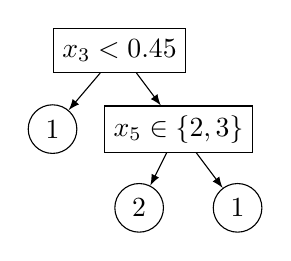
\begin{tikzpicture}
\node (labelleft) [draw,shape=circle,minimum size=16pt] at (2,0) {$2$};
\node (labelright) [draw,shape=circle,minimum size=16pt] at (3.25,0) {$1$};

\node (rootleft) [draw,shape=rectangle,minimum size=16pt] at (2.5,1) {$x_5 \in \{2,3\}$};
\node (rootlabel) [draw,shape=circle,minimum size=16pt] at (0.9,1) {$1$};
\node (root) [draw,shape=rectangle,minimum size=16pt] at (1.75,2) {$x_3 < 0.45$};

\draw[-latex] (root) -- (rootleft);
\draw[-latex] (root) -- (rootlabel);
\draw[-latex] (rootleft) -- (labelleft);
\draw[-latex] (rootleft) -- (labelright);

\end{tikzpicture}
\end{center}
\begin{center}
(a)
\end{center}
\end{minipage}
\hfill
\begin{minipage}{0.65\linewidth}
\begin{center}
\begin{tabular}{c|c|c|c|c|c|}
& Col 1 & Col 2 & Col 3 & Col 4 & Col 5\\
\hline
Row 1 & 1 & 2 & 3 & 6 & 7 \\
\hline
Row 2 & 1 & 0 & 1 & 0 & 0 \\
\hline
Row 3 & 3 & 5 & 0 & 0 & 0 \\
\hline
Row 4 & 1 & 1 & 2 & 2 & 1 \\
\hline
Row 5 & 1 & 0 & 2 & 0 & 0 \\
\hline
Row 6 & 0.45 & 0 & 2 & 0 & 0 \\
\hline
Row 7 &  &  & 3 &  & \\
\hline
\end{tabular}
\end{center}
\begin{center}
(b)
\end{center}
\end{minipage}
\caption{(a) An example tree and its (b) matrix representation. $x$ denotes an example and $x_j$ is the value of the $j$th continuous-valued (resp. categorical) feature in $X_\text{cont}$ (resp. $X_\text{cat}$). In this example all leaf nodes are pure and no training example is misclassified.}
\label{dtree}
\end{figure}


\smallskip
\noindent{\bf Returns}
\smallskip


The matrix corresponding to the learned model as well as the training accuracy (if requested) is written to a file in the format specified. See
details where the structure of the model matrix is described.
Recall that in our implementation $X$ is split into $X_\text{cont}$ and $X_\text{cat}$. If requested, the mappings of the continuous-valued feature-ids in $X_\text{cont}$ (stored at {\tt S\_map}) and the categorical feature-ids in $X_\text{cat}$ (stored at {\tt C\_map}) to the global feature-ids in $X$ will be provided. 
Depending on what arguments are provided during
invocation, the {\tt decision-tree-predict.dml} script may compute one or more of predictions, accuracy and confusion matrix in the requested output format. 

\smallskip
\noindent{\bf Examples}
\smallskip

{\hangindent=\parindent\noindent\tt
	\hml -f decision-tree.dml -nvargs X=/user/biadmin/X.mtx Y=/user/biadmin/Y.mtx
	R=/user/biadmin/R.csv M=/user/biadmin/model.csv
	bins=20 depth=25 num\_leaf=10 num\_samples=3000 impurity=Gini fmt=csv
	
}\smallskip


\noindent To compute predictions:

{\hangindent=\parindent\noindent\tt
	\hml -f decision-tree-predict.dml -nvargs X=/user/biadmin/X.mtx Y=/user/biadmin/Y.mtx R=/user/biadmin/R.csv
	M=/user/biadmin/model.csv  P=/user/biadmin/predictions.csv
	A=/user/biadmin/accuracy.csv CM=/user/biadmin/confusion.csv fmt=csv
	
}\smallskip


%\noindent{\bf References}
%
%\begin{itemize}
%\item B. Panda, J. Herbach, S. Basu, and R. Bayardo. \newblock{PLANET: massively parallel learning of tree ensembles with MapReduce}. In Proceedings of the VLDB Endowment, 2009.
%\item L. Breiman, J. Friedman, R. Olshen, and C. Stone. \newblock{Classification and Regression Trees}. Wadsworth and Brooks, 1984.
%\end{itemize}


\begin{comment}

 Licensed to the Apache Software Foundation (ASF) under one
 or more contributor license agreements.  See the NOTICE file
 distributed with this work for additional information
 regarding copyright ownership.  The ASF licenses this file
 to you under the Apache License, Version 2.0 (the
 "License"); you may not use this file except in compliance
 with the License.  You may obtain a copy of the License at

   http://www.apache.org/licenses/LICENSE-2.0

 Unless required by applicable law or agreed to in writing,
 software distributed under the License is distributed on an
 "AS IS" BASIS, WITHOUT WARRANTIES OR CONDITIONS OF ANY
 KIND, either express or implied.  See the License for the
 specific language governing permissions and limitations
 under the License.

\end{comment}

\subsection{Random Forests}
\label{random_forests}

\noindent{\bf Description}
\smallskip


Random forest is one of the most successful machine learning methods for classification and regression. 
It is an ensemble learning method that creates a model composed of a set of tree models.
This implementation is well-suited to handle large-scale data and builds a random forest model for classification in parallel.\\


\smallskip
\noindent{\bf Usage}
\smallskip

{\hangindent=\parindent\noindent\it%
	{\tt{}-f }path/\/{\tt{}random-forest.dml}
	{\tt{} -nvargs}
	{\tt{} X=}path/file
	{\tt{} Y=}path/file
	{\tt{} R=}path/file
	{\tt{} bins=}integer
	{\tt{} depth=}integer
	{\tt{} num\_leaf=}integer
	{\tt{} num\_samples=}integer
	{\tt{} num\_trees=}integer
	{\tt{} subsamp\_rate=}double
	{\tt{} feature\_subset=}double
	{\tt{} impurity=}Gini$\mid$entropy
	{\tt{} M=}path/file
	{\tt{} C=}path/file
	{\tt{} S\_map=}path/file
	{\tt{} C\_map=}path/file
	{\tt{} fmt=}format
	
}

 \smallskip
 \noindent{\bf Usage: Prediction}
 \smallskip
 
 {\hangindent=\parindent\noindent\it%
 	{\tt{}-f }path/\/{\tt{}random-forest-predict.dml}
 	{\tt{} -nvargs}
 	{\tt{} X=}path/file
 	{\tt{} Y=}path/file
 	{\tt{} R=}path/file
 	{\tt{} M=}path/file
 	{\tt{} C=}path/file
 	{\tt{} P=}path/file
 	{\tt{} A=}path/file
 	{\tt{} OOB=}path/file
 	{\tt{} CM=}path/file
 	{\tt{} fmt=}format
 	
 }\smallskip
 
 
\noindent{\bf Arguments}
\begin{Description}
	\item[{\tt X}:]
	Location (on HDFS) to read the matrix of feature vectors; 
	each row constitutes one feature vector. Note that categorical features in $X$ need to be both recoded and dummy coded.
	\item[{\tt Y}:]
	Location (on HDFS) to read the matrix of (categorical) 
	labels that correspond to feature vectors in $X$. Note that classes are assumed to be both recoded and dummy coded. 
	This argument is optional for prediction. 
	\item[{\tt R}:] (default:\mbox{ }{\tt " "})
	Location (on HDFS) to read matrix $R$ which for each feature in $X$ contains column-ids (first column), start indices (second column), and end indices (third column).
	If $R$ is not provided by default all features are assumed to be continuous-valued.   
	\item[{\tt bins}:] (default:\mbox{ }{\tt 20})
	Number of thresholds to choose for each continuous-valued feature (determined by equi-height binning). 
	\item[{\tt depth}:] (default:\mbox{ }{\tt 25})
	Maximum depth of the learned trees in the random forest model
	\item[{\tt num\_leaf}:] (default:\mbox{ }{\tt 10})
	Parameter that controls pruning. The tree
	is not expanded if a node receives less than {\tt num\_leaf} training examples.
	\item[{\tt num\_samples}:] (default:\mbox{ }{\tt 3000})
	Parameter that decides when to switch to in-memory building of the subtrees in each tree of the random forest model. 
	If a node $v$ receives less than {\tt num\_samples}
	training examples then this implementation switches to an in-memory subtree
	building procedure to build the subtree under $v$ in its entirety.
	\item[{\tt num\_trees}:] (default:\mbox{ }{\tt 10})
	Number of trees to be learned in the random forest model
	\item[{\tt subsamp\_rate}:] (default:\mbox{ }{\tt 1.0})
	Parameter controlling the size of each tree in the random forest model; samples are selected from a Poisson distribution with parameter {\tt subsamp\_rate}.
	\item[{\tt feature\_subset}:] (default:\mbox{ }{\tt 0.5})
	Parameter that controls the number of feature used as candidates for splitting at each tree node as a power of the number of features in the data, i.e., assuming the training set has $D$ features $D^{\tt feature\_subset}$ are used at each tree node.
	\item[{\tt impurity}:] (default:\mbox{ }{\tt "Gini"})
	Impurity measure used at internal nodes of the trees in the random forest model for selecting which features to split on. Possible value are entropy or Gini.
	\item[{\tt M}:] 
	Location (on HDFS) to write matrix $M$ containing the learned random forest (see Section~\ref{sec:decision_trees} and below for the schema) 
	\item[{\tt C}:] (default:\mbox{ }{\tt " "})
	Location (on HDFS) to store the number of counts (generated according to a Poisson distribution with parameter {\tt subsamp\_rate}) for each feature vector. Note that this argument is optional. If Out-Of-Bag (OOB) error estimate needs to be computed this parameter is passed as input to {\tt random-forest-predict.dml}. 
	\item[{\tt A}:] (default:\mbox{ }{\tt " "})
	Location (on HDFS) to store the testing accuracy (\%) from a 
	held-out test set during prediction. Note that this argument is optional.
	\item[{\tt OOB}:] (default:\mbox{ }{\tt " "})
	Location (on HDFS) to store the Out-Of-Bag (OOB) error estimate of the training set. Note that the matrix of sample counts (stored at {\tt C}) needs to be provided for computing OOB error estimate. Note that this argument is optional.
	\item[{\tt P}:] 
	Location (on HDFS) to store predictions for a held-out test set
	\item[{\tt CM}:] (default:\mbox{ }{\tt " "})
	Location (on HDFS) to store the confusion matrix computed using a held-out test set. Note that this argument is optional.
	\item[{\tt S\_map}:] (default:\mbox{ }{\tt " "})
	Location (on HDFS) to write the mappings from the continuous-valued feature-ids to the global feature-ids in $X$ (see below for details). Note that this argument is optional.
	\item[{\tt C\_map}:] (default:\mbox{ }{\tt " "})
	Location (on HDFS) to write the mappings from the categorical feature-ids to the global feature-ids in $X$ (see below for details). Note that this argument is optional.
	\item[{\tt fmt}:] (default:\mbox{ }{\tt "text"})
	Matrix file output format, such as {\tt text}, {\tt mm}, or {\tt csv};
	see read/write functions in SystemML Language Reference for details.
\end{Description}


 \noindent{\bf Details}
 \smallskip

Random forests~\cite{Breiman01:rforest} are learning algorithms for ensembles of decision trees. 
The main idea is to build a number of decision trees on bootstrapped training samples, i.e., by taking repeatedly samples from a (single) training set. 
Moreover, instead of considering all the features when building the trees only a random subset of the features---typically $\approx \sqrt{D}$, where $D$ is the number of features---is chosen each time a split test at a tree node is performed. 
This procedure {\it decorrelates} the trees and makes it less prone to overfitting. 
To build decision trees we utilize the techniques discussed in Section~\ref{sec:decision_trees} proposed in~\cite{PandaHBB09:dtree}; 
the implementation details are similar to those of the decision trees script.
Below we review some features of our implementation which differ from {\tt decision-tree.dml}.


\textbf{Bootstrapped sampling.} 
Each decision tree is fitted to a bootstrapped training set sampled with replacement (WR).  
To improve efficiency, we generate $N$ sample counts according to a Poisson distribution with parameter {\tt subsamp\_rate},
where $N$ denotes the total number of training points.
These sample counts approximate WR sampling when $N$ is large enough and are generated upfront for each decision tree.


\textbf{Bagging.}
Decision trees suffer from {\it high variance} resulting in different models whenever trained on a random subsets of the data points.  
{\it Bagging} is a general-purpose method to reduce the variance of a statistical learning method like decision trees.
In the context of decision trees (for classification), for a given test feature vector 
the prediction is computed by taking a {\it majority vote}: the overall prediction is the most commonly occurring class among all the tree predictions.

 
\textbf{Out-Of-Bag error estimation.} 
Note that each bagged tree in a random forest model is trained on a subset (around $\frac{2}{3}$) of the observations (i.e., feature vectors).
The remaining ($\frac{1}{3}$ of the) observations not used for training is called the {\it Out-Of-Bag} (OOB) observations. 
This gives us a straightforward way to estimate the test error: to predict the class label of each test observation $i$ we use the trees in which $i$ was OOB.
Our {\tt random-forest-predict.dml} script provides the OOB error estimate for a given training set if requested.  


\textbf{Description of the model.} 
Similar to decision trees, the learned random forest model is presented in a matrix $M$  with at least 7 rows.
The information stored in the model is similar to that of decision trees with the difference that the tree-ids are stored
in the second row and rows $2,3,\ldots$ from the decision tree model are shifted by one. See Section~\ref{sec:decision_trees} for a description of the model.


\smallskip
\noindent{\bf Returns}
\smallskip


The matrix corresponding to the learned model is written to a file in the format specified. See Section~\ref{sec:decision_trees} where the details about the structure of the model matrix is described.
Similar to {\tt decision-tree.dml}, $X$ is split into $X_\text{cont}$ and $X_\text{cat}$. 
If requested, the mappings of the continuous feature-ids in $X_\text{cont}$ (stored at {\tt S\_map}) as well as the categorical feature-ids in $X_\text{cat}$ (stored at {\tt C\_map}) to the global feature-ids in $X$ will be provided. 
The {\tt random-forest-predict.dml} script may compute one or more of
predictions, accuracy, confusion matrix, and OOB error estimate in the requested output format depending on the input arguments used. 
 


\smallskip
\noindent{\bf Examples}
\smallskip

{\hangindent=\parindent\noindent\tt
	\hml -f random-forest.dml -nvargs X=/user/biadmin/X.mtx Y=/user/biadmin/Y.mtx
	R=/user/biadmin/R.csv M=/user/biadmin/model.csv
	bins=20 depth=25 num\_leaf=10 num\_samples=3000 num\_trees=10 impurity=Gini fmt=csv
	
}\smallskip


\noindent To compute predictions:

{\hangindent=\parindent\noindent\tt
	\hml -f random-forest-predict.dml -nvargs X=/user/biadmin/X.mtx Y=/user/biadmin/Y.mtx R=/user/biadmin/R.csv
	M=/user/biadmin/model.csv P=/user/biadmin/predictions.csv
	A=/user/biadmin/accuracy.csv CM=/user/biadmin/confusion.csv fmt=csv
	
}\smallskip


%\noindent{\bf References}
%
%\begin{itemize}
%\item B. Panda, J. Herbach, S. Basu, and R. Bayardo. \newblock{PLANET: massively parallel learning of tree ensembles with MapReduce}. In Proceedings of the VLDB Endowment, 2009.
%\item L. Breiman. \newblock{Random Forests}. Machine Learning, 45(1), 5--32, 2001.
%\end{itemize}


%%%%%%%%%%%%%%%%%%%%%%%%%%%%%%%%%%%%%%%%%%%%%%%%%%%%%%%%%%%%%%%%%%%%%%%%%%%%%%%%
\section{Clustering}
%%%%%%%%%%%%%%%%%%%%%%%%%%%%%%%%%%%%%%%%%%%%%%%%%%%%%%%%%%%%%%%%%%%%%%%%%%%%%%%%

\begin{comment}

 Licensed to the Apache Software Foundation (ASF) under one
 or more contributor license agreements.  See the NOTICE file
 distributed with this work for additional information
 regarding copyright ownership.  The ASF licenses this file
 to you under the Apache License, Version 2.0 (the
 "License"); you may not use this file except in compliance
 with the License.  You may obtain a copy of the License at

   http://www.apache.org/licenses/LICENSE-2.0

 Unless required by applicable law or agreed to in writing,
 software distributed under the License is distributed on an
 "AS IS" BASIS, WITHOUT WARRANTIES OR CONDITIONS OF ANY
 KIND, either express or implied.  See the License for the
 specific language governing permissions and limitations
 under the License.

\end{comment}

\subsection{K-Means Clustering}

\noindent{\bf Description}
\smallskip

Given a collection of $n$ records with a pairwise similarity measure,
the goal of clustering is to assign a category label to each record so that
similar records tend to get the same label.  In contrast to multinomial
logistic regression, clustering is an \emph{unsupervised}\/ learning problem
with neither category assignments nor label interpretations given in advance.
In $k$-means clustering, the records $x_1, x_2, \ldots, x_n$ are numerical
feature vectors of $\dim x_i = m$ with the squared Euclidean distance 
$\|x_i - x_{i'}\|_2^2$ as the similarity measure.  We want to partition
$\{x_1, \ldots, x_n\}$ into $k$ clusters $\{S_1, \ldots, S_k\}$ so that
the aggregated squared distance from records to their cluster means is
minimized:
\begin{equation}
\textrm{WCSS}\,\,=\,\, \sum_{i=1}^n \,\big\|x_i - \mean(S_j: x_i\in S_j)\big\|_2^2 \,\,\to\,\,\min
\label{eqn:WCSS}
\end{equation}
The aggregated distance measure in~(\ref{eqn:WCSS}) is called the
\emph{within-cluster sum of squares}~(WCSS).  It can be viewed as a measure
of residual variance that remains in the data after the clustering assignment,
conceptually similar to the residual sum of squares~(RSS) in linear regression.
However, unlike for the RSS, the minimization of~(\ref{eqn:WCSS}) is an NP-hard 
problem~\cite{AloiseDHP2009:kmeans}.

Rather than searching for the global optimum in~(\ref{eqn:WCSS}), a heuristic algorithm
called Lloyd's algorithm is typically used.  This iterative algorithm maintains
and updates a set of $k$~\emph{centroids} $\{c_1, \ldots, c_k\}$, one centroid per cluster.
It defines each cluster $S_j$ as the set of all records closer to~$c_j$ than
to any other centroid.  Each iteration of the algorithm reduces the WCSS in two steps:
\begin{Enumerate}
\item Assign each record to the closest centroid, making $\mean(S_j)\neq c_j$;
\label{step:kmeans:recluster}
\item Reset each centroid to its cluster's mean: $c_j := \mean(S_j)$.
\label{step:kmeans:recenter}
\end{Enumerate}
After Step~\ref{step:kmeans:recluster} the centroids are generally different from the cluster
means, so we can compute another ``within-cluster sum of squares'' based on the centroids:
\begin{equation}
\textrm{WCSS\_C}\,\,=\,\, \sum_{i=1}^n \,\big\|x_i - \mathop{\textrm{centroid}}(S_j: x_i\in S_j)\big\|_2^2
\label{eqn:WCSS:C}
\end{equation}
This WCSS\_C after Step~\ref{step:kmeans:recluster} is less than the means-based WCSS
before Step~\ref{step:kmeans:recluster} (or equal if convergence achieved), and in
Step~\ref{step:kmeans:recenter} the WCSS cannot exceed the WCSS\_C for \emph{the same}
clustering; hence the WCSS reduction.

Exact convergence is reached when each record becomes closer to its
cluster's mean than to any other cluster's mean, so there are no more re-assignments
and the centroids coincide with the means.  In practice, iterations may be stopped
when the reduction in WCSS (or in WCSS\_C) falls below a minimum threshold, or upon
reaching the maximum number of iterations.  The initialization of the centroids is also
an important part of the algorithm.  The smallest WCSS obtained by the algorithm is not
the global minimum and varies depending on the initial centroids.  We implement multiple
parallel runs with different initial centroids and report the best result.

\Paragraph{Scoring} 
Our scoring script evaluates the clustering output by comparing it with a known category
assignment.  Since cluster labels have no prior correspondence to the categories, we
cannot count ``correct'' and ``wrong'' cluster assignments.  Instead, we quantify them in
two ways:
\begin{Enumerate}
\item Count how many same-category and different-category pairs of records end up in the
same cluster or in different clusters;
\item For each category, count the prevalence of its most common cluster; for each
cluster, count the prevalence of its most common category.
\end{Enumerate}
The number of categories and the number of clusters ($k$) do not have to be equal.  
A same-category pair of records clustered into the same cluster is viewed as a
``true positive,'' a different-category pair clustered together is a ``false positive,''
a same-category pair clustered apart is a ``false negative''~etc.


\smallskip
\noindent{\bf Usage: K-means Script}
\smallskip

{\hangindent=\parindent\noindent\it%
{\tt{}-f }path/\/{\tt{}Kmeans.dml}
{\tt{} -nvargs}
{\tt{} X=}path/file
{\tt{} C=}path/file
{\tt{} k=}int
{\tt{} runs=}int
{\tt{} maxi=}int
{\tt{} tol=}double
{\tt{} samp=}int
{\tt{} isY=}int
{\tt{} Y=}path/file
{\tt{} fmt=}format
{\tt{} verb=}int

}

\smallskip
\noindent{\bf Usage: K-means Scoring/Prediction}
\smallskip

{\hangindent=\parindent\noindent\it%
{\tt{}-f }path/\/{\tt{}Kmeans-predict.dml}
{\tt{} -nvargs}
{\tt{} X=}path/file
{\tt{} C=}path/file
{\tt{} spY=}path/file
{\tt{} prY=}path/file
{\tt{} fmt=}format
{\tt{} O=}path/file

}

\smallskip
\noindent{\bf Arguments}
\begin{Description}
\item[{\tt X}:]
Location to read matrix $X$ with the input data records as rows
\item[{\tt C}:] (default:\mbox{ }{\tt "C.mtx"})
Location to store the output matrix with the best available cluster centroids as rows
\item[{\tt k}:]
Number of clusters (and centroids)
\item[{\tt runs}:] (default:\mbox{ }{\tt 10})
Number of parallel runs, each run with different initial centroids
\item[{\tt maxi}:] (default:\mbox{ }{\tt 1000})
Maximum number of iterations per run
\item[{\tt tol}:] (default:\mbox{ }{\tt 0.000001})
Tolerance (epsilon) for single-iteration WCSS\_C change ratio
\item[{\tt samp}:] (default:\mbox{ }{\tt 50})
Average number of records per centroid in data samples used in the centroid
initialization procedure
\item[{\tt Y}:] (default:\mbox{ }{\tt "Y.mtx"})
Location to store the one-column matrix $Y$ with the best available mapping of
records to clusters (defined by the output centroids)
\item[{\tt isY}:] (default:\mbox{ }{\tt 0})
{\tt 0} = do not write matrix~$Y$,  {\tt 1} = write~$Y$
\item[{\tt fmt}:] (default:\mbox{ }{\tt "text"})
Matrix file output format, such as {\tt text}, {\tt mm}, or {\tt csv};
see read/write functions in SystemML Language Reference for details.
\item[{\tt verb}:] (default:\mbox{ }{\tt 0})
{\tt 0} = do not print per-iteration statistics for each run, {\tt 1} = print them
(the ``verbose'' option)
\end{Description}
\smallskip
\noindent{\bf Arguments --- Scoring/Prediction}
\begin{Description}
\item[{\tt X}:] (default:\mbox{ }{\tt " "})
Location to read matrix $X$ with the input data records as rows,
optional when {\tt prY} input is provided
\item[{\tt C}:] (default:\mbox{ }{\tt " "})
Location to read matrix $C$ with cluster centroids as rows, optional
when {\tt prY} input is provided; NOTE: if both {\tt X} and {\tt C} are
provided, {\tt prY} is an output, not input
\item[{\tt spY}:] (default:\mbox{ }{\tt " "})
Location to read a one-column matrix with the externally specified ``true''
assignment of records (rows) to categories, optional for prediction without
scoring
\item[{\tt prY}:] (default:\mbox{ }{\tt " "})
Location to read (or write, if {\tt X} and {\tt C} are present) a
column-vector with the predicted assignment of rows to clusters;
NOTE: No prior correspondence is assumed between the predicted
cluster labels and the externally specified categories
\item[{\tt fmt}:] (default:\mbox{ }{\tt "text"})
Matrix file output format for {\tt prY}, such as {\tt text}, {\tt mm},
or {\tt csv}; see read/write functions in SystemML Language Reference
for details
\item[{\tt O}:] (default:\mbox{ }{\tt " "})
Location to write the output statistics defined in 
Table~\ref{table:kmeans:predict:stats}, by default print them to the
standard output
\end{Description}


\begin{table}[t]\small\centerline{%
\begin{tabular}{|lcl|}
\hline
Name & CID & Meaning \\
\hline
{\tt TSS}             &     & Total Sum of Squares (from the total mean) \\
{\tt WCSS\_M}         &     & Within-Cluster  Sum of Squares (means as centers) \\
{\tt WCSS\_M\_PC}     &     & Within-Cluster  Sum of Squares (means), in \% of TSS \\
{\tt BCSS\_M}         &     & Between-Cluster Sum of Squares (means as centers) \\
{\tt BCSS\_M\_PC}     &     & Between-Cluster Sum of Squares (means), in \% of TSS \\
\hline
{\tt WCSS\_C}         &     & Within-Cluster  Sum of Squares (centroids as centers) \\
{\tt WCSS\_C\_PC}     &     & Within-Cluster  Sum of Squares (centroids), \% of TSS \\
{\tt BCSS\_C}         &     & Between-Cluster Sum of Squares (centroids as centers) \\
{\tt BCSS\_C\_PC}     &     & Between-Cluster Sum of Squares (centroids), \% of TSS \\
\hline
{\tt TRUE\_SAME\_CT}  &     & Same-category pairs predicted as Same-cluster, count \\
{\tt TRUE\_SAME\_PC}  &     & Same-category pairs predicted as Same-cluster, \% \\
{\tt TRUE\_DIFF\_CT}  &     & Diff-category pairs predicted as Diff-cluster, count \\
{\tt TRUE\_DIFF\_PC}  &     & Diff-category pairs predicted as Diff-cluster, \% \\
{\tt FALSE\_SAME\_CT} &     & Diff-category pairs predicted as Same-cluster, count \\
{\tt FALSE\_SAME\_PC} &     & Diff-category pairs predicted as Same-cluster, \% \\
{\tt FALSE\_DIFF\_CT} &     & Same-category pairs predicted as Diff-cluster, count \\
{\tt FALSE\_DIFF\_PC} &     & Same-category pairs predicted as Diff-cluster, \% \\
\hline
{\tt SPEC\_TO\_PRED}  & $+$ & For specified category, the best predicted cluster id \\
{\tt SPEC\_FULL\_CT}  & $+$ & For specified category, its full count \\
{\tt SPEC\_MATCH\_CT} & $+$ & For specified category, best-cluster matching count \\
{\tt SPEC\_MATCH\_PC} & $+$ & For specified category, \% of matching to full count \\
{\tt PRED\_TO\_SPEC}  & $+$ & For predicted cluster, the best specified category id \\
{\tt PRED\_FULL\_CT}  & $+$ & For predicted cluster, its full count \\
{\tt PRED\_MATCH\_CT} & $+$ & For predicted cluster, best-category matching count \\
{\tt PRED\_MATCH\_PC} & $+$ & For predicted cluster, \% of matching to full count \\
\hline
\end{tabular}}
\caption{The {\tt O}-file for {\tt Kmeans-predict} provides the output statistics
in CSV format, one per line, in the following format: (NAME, [CID], VALUE).  Note:
the 1st group statistics are given if {\tt X} input is available;
the 2nd group statistics are given if {\tt X} and {\tt C} inputs are available;
the 3rd and 4th group statistics are given if {\tt spY} input is available;
only the 4th group statistics contain a nonempty CID value;
when present, CID contains either the specified category label or the
predicted cluster label.}
\label{table:kmeans:predict:stats}
\end{table}


\noindent{\bf Details}
\smallskip

Our clustering script proceeds in 3~stages: centroid initialization,
parallel $k$-means iterations, and the best-available output generation.
Centroids are initialized at random from the input records (the rows of~$X$),
biased towards being chosen far apart from each other.  The initialization
method is based on the {\tt k-means++} heuristic from~\cite{ArthurVassilvitskii2007:kmeans},
with one important difference: to reduce the number of passes through~$X$,
we take a small sample of $X$ and run the {\tt k-means++} heuristic over
this sample.  Here is, conceptually, our centroid initialization algorithm
for one clustering run:
\begin{Enumerate}
\item Sample the rows of~$X$ uniformly at random, picking each row with probability
$p = ks / n$ where
\begin{Itemize}
\item $k$~is the number of centroids, 
\item $n$~is the number of records, and
\item $s$~is the {\tt samp} input parameter.
\end{Itemize}
If $ks \geq n$, the entire $X$ is used in place of its sample.
\item Choose the first centroid uniformly at random from the sampled rows.
\item Choose each subsequent centroid from the sampled rows, at random, with
probability proportional to the squared Euclidean distance between the row and
the nearest already-chosen centroid.
\end{Enumerate}
The sampling of $X$ and the selection of centroids are performed independently
and in parallel for each run of the $k$-means algorithm.  When we sample the
rows of~$X$, rather than tossing a random coin for each row, we compute the
number of rows to skip until the next sampled row as $\lceil \log(u) / \log(1 - p) \rceil$
where $u\in (0, 1)$ is uniformly random.  This time-saving trick works because
\begin{equation*}
\Prob [k-1 < \log_{1-p}(u) < k] \,\,=\,\, p(1-p)^{k-1} \,\,=\,\,
\Prob [\textrm{skip $k-1$ rows}]
\end{equation*}
However, it requires us to estimate the maximum sample size, which we set
near~$ks + 10\sqrt{ks}$ to make it generous enough.

Once we selected the initial centroid sets, we start the $k$-means iterations
independently in parallel for all clustering runs.  The number of clustering runs
is given as the {\tt runs} input parameter.  Each iteration of each clustering run
performs the following steps:
\begin{Itemize}
\item Compute the centroid-dependent part of squared Euclidean distances from
all records (rows of~$X$) to each of the $k$~centroids using matrix product;
\item Take the minimum of the above for each record;
\item Update the current within-cluster sum of squares (WCSS) value, with centroids
substituted instead of the means for efficiency;
\item Check the convergence criterion:\hfil
$\textrm{WCSS}_{\mathrm{old}} - \textrm{WCSS}_{\mathrm{new}} < \eps\cdot\textrm{WCSS}_{\mathrm{new}}$\linebreak
as well as the number of iterations limit;
\item Find the closest centroid for each record, sharing equally any records with multiple
closest centroids;
\item Compute the number of records closest to each centroid, checking for ``runaway''
centroids with no records left (in which case the run fails);
\item Compute the new centroids by averaging the records in their clusters.
\end{Itemize}
When a termination condition is satisfied, we store the centroids and the WCSS value
and exit this run.  A run has to satisfy the WCSS convergence criterion to be considered
successful.  Upon the termination of all runs, we select the smallest WCSS value among
the successful runs, and write out this run's centroids.  If requested, we also compute
the cluster assignment of all records in~$X$, using integers from 1 to~$k$ as the cluster
labels.  The scoring script can then be used to compare the cluster assignment with
an externally specified category assignment.

\smallskip
\noindent{\bf Returns}
\smallskip

We output the $k$ centroids for the best available clustering, i.~e.\ whose WCSS
is the smallest of all successful runs.
The centroids are written as the rows of the $k\,{\times}\,m$-matrix into the output
file whose path/name was provided as the ``{\tt C}'' input argument.  If the input
parameter ``{\tt isY}'' was set to~{\tt 1}, we also output the one-column matrix with
the cluster assignment for all the records.  This assignment is written into the
file whose path/name was provided as the ``{\tt Y}'' input argument.
The best WCSS value, as well as some information about the performance of the other
runs, is printed during the script execution.  The scoring script {\tt Kmeans-predict}
prints all its results in a self-explanatory manner, as defined in
Table~\ref{table:kmeans:predict:stats}.


\smallskip
\noindent{\bf Examples}
\smallskip

{\hangindent=\parindent\noindent\tt
\hml -f Kmeans.dml -nvargs X=/user/biadmin/X.mtx k=5 C=/user/biadmin/centroids.mtx fmt=csv

}

{\hangindent=\parindent\noindent\tt
\hml -f Kmeans.dml -nvargs X=/user/biadmin/X.mtx k=5 runs=100 maxi=5000 
tol=0.00000001 samp=20 C=/user/biadmin/centroids.mtx isY=1 Y=/user/biadmin/Yout.mtx verb=1

}
\noindent To predict {\tt Y} given {\tt X} and {\tt C}:

{\hangindent=\parindent\noindent\tt
\hml -f Kmeans-predict.dml -nvargs X=/user/biadmin/X.mtx
         C=/user/biadmin/C.mtx prY=/user/biadmin/PredY.mtx O=/user/biadmin/stats.csv

}
\noindent To compare ``actual'' labels {\tt spY} with ``predicted'' labels given {\tt X} and {\tt C}:

{\hangindent=\parindent\noindent\tt
\hml -f Kmeans-predict.dml -nvargs X=/user/biadmin/X.mtx
         C=/user/biadmin/C.mtx spY=/user/biadmin/Y.mtx O=/user/biadmin/stats.csv

}
\noindent To compare ``actual'' labels {\tt spY} with given ``predicted'' labels {\tt prY}:

{\hangindent=\parindent\noindent\tt
\hml -f Kmeans-predict.dml -nvargs spY=/user/biadmin/Y.mtx prY=/user/biadmin/PredY.mtx O=/user/biadmin/stats.csv

}

\smallskip
\noindent{\bf References}
\begin{itemize}
\item
D.~Aloise, A.~Deshpande, P.~Hansen, and P.~Popat.
\newblock {NP}-hardness of {E}uclidean sum-of-squares clustering.
\newblock {\em Machine Learning}, 75(2):245--248, May 2009.
\item
D.~Arthur and S.~Vassilvitskii.
\newblock {\tt k-means++}: The advantages of careful seeding.
\newblock In {\em Proceedings of the 18th Annual {ACM-SIAM} Symposium on
  Discrete Algorithms ({SODA}~2007)}, pages 1027--1035, New Orleans~{LA},
  {USA}, January 7--9 2007.
\end{itemize}


%%%%%%%%%%%%%%%%%%%%%%%%%%%%%%%%%%%%%%%%%%%%%%%%%%%%%%%%%%%%%%%%%%%%%%%%%%%%%%%%
\section{Regression}
%%%%%%%%%%%%%%%%%%%%%%%%%%%%%%%%%%%%%%%%%%%%%%%%%%%%%%%%%%%%%%%%%%%%%%%%%%%%%%%%

\begin{comment}

 Licensed to the Apache Software Foundation (ASF) under one
 or more contributor license agreements.  See the NOTICE file
 distributed with this work for additional information
 regarding copyright ownership.  The ASF licenses this file
 to you under the Apache License, Version 2.0 (the
 "License"); you may not use this file except in compliance
 with the License.  You may obtain a copy of the License at

   http://www.apache.org/licenses/LICENSE-2.0

 Unless required by applicable law or agreed to in writing,
 software distributed under the License is distributed on an
 "AS IS" BASIS, WITHOUT WARRANTIES OR CONDITIONS OF ANY
 KIND, either express or implied.  See the License for the
 specific language governing permissions and limitations
 under the License.

\end{comment}

\subsection{Linear Regression}
\label{sec:LinReg}

\noindent{\bf Description}
\smallskip

Linear Regression scripts are used to model the relationship between one numerical
response variable and one or more explanatory (feature) variables.
The scripts are given a dataset $(X, Y) = (x_i, y_i)_{i=1}^n$ where $x_i$ is a
numerical vector of feature variables and $y_i$ is a numerical response value for
each training data record.  The feature vectors are provided as a matrix $X$ of size
$n\,{\times}\,m$, where $n$ is the number of records and $m$ is the number of features.
The observed response values are provided as a 1-column matrix~$Y$, with a numerical
value $y_i$ for each~$x_i$ in the corresponding row of matrix~$X$.

In linear regression, we predict the distribution of the response~$y_i$ based on
a fixed linear combination of the features in~$x_i$.  We assume that
there exist constant regression coefficients $\beta_0, \beta_1, \ldots, \beta_m$
and a constant residual variance~$\sigma^2$ such that
\begin{equation}
y_i \sim \Normal(\mu_i, \sigma^2) \,\,\,\,\textrm{where}\,\,\,\,
\mu_i \,=\, \beta_0 + \beta_1 x_{i,1} + \ldots + \beta_m x_{i,m}
\label{eqn:linregdef}
\end{equation}
Distribution $y_i \sim \Normal(\mu_i, \sigma^2)$ models the ``unexplained'' residual
noise and is assumed independent across different records.

The goal is to estimate the regression coefficients and the residual variance.
Once they are accurately estimated, we can make predictions about $y_i$ given~$x_i$
in new records.  We can also use the $\beta_j$'s to analyze the influence of individual
features on the response value, and assess the quality of this model by comparing
residual variance in the response, left after prediction, with its total variance.

There are two scripts in our library, both doing the same estimation, but using different
computational methods.  Depending on the size and the sparsity of the feature matrix~$X$,
one or the other script may be more efficient.  The ``direct solve'' script
{\tt LinearRegDS} is more efficient when the number of features $m$ is relatively small
($m \sim 1000$ or less) and matrix~$X$ is either tall or fairly dense
(has~${\gg}\:m^2$ nonzeros); otherwise, the ``conjugate gradient'' script {\tt LinearRegCG}
is more efficient.  If $m > 50000$, use only {\tt LinearRegCG}.

\smallskip
\noindent{\bf Usage}
\smallskip

{\hangindent=\parindent\noindent\it%
{\tt{}-f }path/\/{\tt{}LinearRegDS.dml}
{\tt{} -nvargs}
{\tt{} X=}path/file
{\tt{} Y=}path/file
{\tt{} B=}path/file
{\tt{} O=}path/file
{\tt{} icpt=}int
{\tt{} reg=}double
{\tt{} fmt=}format

}\smallskip
{\hangindent=\parindent\noindent\it%
{\tt{}-f }path/\/{\tt{}LinearRegCG.dml}
{\tt{} -nvargs}
{\tt{} X=}path/file
{\tt{} Y=}path/file
{\tt{} B=}path/file
{\tt{} O=}path/file
{\tt{} Log=}path/file
{\tt{} icpt=}int
{\tt{} reg=}double
{\tt{} tol=}double
{\tt{} maxi=}int
{\tt{} fmt=}format

}

\smallskip
\noindent{\bf Arguments}
\begin{Description}
\item[{\tt X}:]
Location (on HDFS) to read the matrix of feature vectors, each row constitutes
one feature vector
\item[{\tt Y}:]
Location to read the 1-column matrix of response values
\item[{\tt B}:]
Location to store the estimated regression parameters (the $\beta_j$'s), with the
intercept parameter~$\beta_0$ at position {\tt B[}$m\,{+}\,1$, {\tt 1]} if available
\item[{\tt O}:] (default:\mbox{ }{\tt " "})
Location to store the CSV-file of summary statistics defined in
Table~\ref{table:linreg:stats}, the default is to print it to the standard output
\item[{\tt Log}:] (default:\mbox{ }{\tt " "}, {\tt LinearRegCG} only)
Location to store iteration-specific variables for monitoring and debugging purposes,
see Table~\ref{table:linreg:log} for details.
\item[{\tt icpt}:] (default:\mbox{ }{\tt 0})
Intercept presence and shifting/rescaling the features in~$X$:\\
{\tt 0} = no intercept (hence no~$\beta_0$), no shifting or rescaling of the features;\\
{\tt 1} = add intercept, but do not shift/rescale the features in~$X$;\\
{\tt 2} = add intercept, shift/rescale the features in~$X$ to mean~0, variance~1
\item[{\tt reg}:] (default:\mbox{ }{\tt 0.000001})
L2-regularization parameter~\mbox{$\lambda\geq 0$}; set to nonzero for highly dependent,
sparse, or numerous ($m \gtrsim n/10$) features
\item[{\tt tol}:] (default:\mbox{ }{\tt 0.000001}, {\tt LinearRegCG} only)
Tolerance \mbox{$\eps\geq 0$} used in the convergence criterion: we terminate conjugate
gradient iterations when the $\beta$-residual reduces in L2-norm by this factor
\item[{\tt maxi}:] (default:\mbox{ }{\tt 0}, {\tt LinearRegCG} only)
Maximum number of conjugate gradient iterations, or~0 if no maximum
limit provided
\item[{\tt fmt}:] (default:\mbox{ }{\tt "text"})
Matrix file output format, such as {\tt text}, {\tt mm}, or {\tt csv};
see read/write functions in SystemML Language Reference for details.
\end{Description}


\begin{table}[t]\small\centerline{%
\begin{tabular}{|ll|}
\hline
Name & Meaning \\
\hline
{\tt AVG\_TOT\_Y}          & Average of the response value $Y$ \\
{\tt STDEV\_TOT\_Y}        & Standard Deviation of the response value $Y$ \\
{\tt AVG\_RES\_Y}          & Average of the residual $Y - \mathop{\mathrm{pred}}(Y|X)$, i.e.\ residual bias \\
{\tt STDEV\_RES\_Y}        & Standard Deviation of the residual $Y - \mathop{\mathrm{pred}}(Y|X)$ \\
{\tt DISPERSION}           & GLM-style dispersion, i.e.\ residual sum of squares / \#deg.\ fr. \\
{\tt PLAIN\_R2}            & Plain $R^2$ of residual with bias included vs.\ total average \\
{\tt ADJUSTED\_R2}         & Adjusted $R^2$ of residual with bias included vs.\ total average \\
{\tt PLAIN\_R2\_NOBIAS}    & Plain $R^2$ of residual with bias subtracted vs.\ total average \\
{\tt ADJUSTED\_R2\_NOBIAS} & Adjusted $R^2$ of residual with bias subtracted vs.\ total average \\
{\tt PLAIN\_R2\_VS\_0}     & ${}^*$Plain $R^2$ of residual with bias included vs.\ zero constant \\
{\tt ADJUSTED\_R2\_VS\_0}  & ${}^*$Adjusted $R^2$ of residual with bias included vs.\ zero constant \\
\hline
\multicolumn{2}{r}{${}^{*\mathstrut}$ The last two statistics are only printed if there is no intercept ({\tt icpt=0})} \\
\end{tabular}}
\caption{Besides~$\beta$, linear regression scripts compute a few summary statistics
listed above.  The statistics are provided in CSV format, one comma-separated name-value
pair per each line.}
\label{table:linreg:stats}
\end{table}

\begin{table}[t]\small\centerline{%
\begin{tabular}{|ll|}
\hline
Name & Meaning \\
\hline
{\tt CG\_RESIDUAL\_NORM}  & L2-norm of conjug.\ grad.\ residual, which is $A \pxp \beta - t(X) \pxp y$ \\
                          & where $A = t(X) \pxp X + \diag (\lambda)$, or a similar quantity \\
{\tt CG\_RESIDUAL\_RATIO} & Ratio of current L2-norm of conjug.\ grad.\ residual over the initial \\
\hline
\end{tabular}}
\caption{
The {\tt Log} file for {\tt{}LinearRegCG} script contains the above \mbox{per-}iteration
variables in CSV format, each line containing triple (Name, Iteration\#, Value) with
Iteration\# being~0 for initial values.}
\label{table:linreg:log}
\end{table}


\noindent{\bf Details}
\smallskip

To solve a linear regression problem over feature matrix~$X$ and response vector~$Y$,
we can find coefficients $\beta_0, \beta_1, \ldots, \beta_m$ and $\sigma^2$ that maximize
the joint likelihood of all $y_i$ for $i=1\ldots n$, defined by the assumed statistical
model~(\ref{eqn:linregdef}).  Since the joint likelihood of the independent
$y_i \sim \Normal(\mu_i, \sigma^2)$ is proportional to the product of
$\exp\big({-}\,(y_i - \mu_i)^2 / (2\sigma^2)\big)$, we can take the logarithm of this
product, then multiply by $-2\sigma^2 < 0$ to obtain a least squares problem:
\begin{equation}
\sum_{i=1}^n \, (y_i - \mu_i)^2 \,\,=\,\, 
\sum_{i=1}^n \Big(y_i - \beta_0 - \sum_{j=1}^m \beta_j x_{i,j}\Big)^2
\,\,\to\,\,\min
\label{eqn:linregls}
\end{equation}
This may not be enough, however.  The minimum may sometimes be attained over infinitely many
$\beta$-vectors, for example if $X$ has an all-0 column, or has linearly dependent columns,
or has fewer rows than columns~\mbox{($n < m$)}.  Even if~(\ref{eqn:linregls}) has a unique
solution, other $\beta$-vectors may be just a little suboptimal\footnote{Smaller likelihood
difference between two models suggests less statistical evidence to pick one model over the
other.}, yet give significantly different predictions for new feature vectors.  This results
in \emph{overfitting}: prediction error for the training data ($X$ and~$Y$) is much smaller
than for the test data (new records).

Overfitting and degeneracy in the data is commonly mitigated by adding a regularization penalty
term to the least squares function:
\begin{equation}
\sum_{i=1}^n \Big(y_i - \beta_0 - \sum_{j=1}^m \beta_j x_{i,j}\Big)^2
\,+\,\, \lambda \sum_{j=1}^m \beta_j^2
\,\,\to\,\,\min
\label{eqn:linreglsreg}
\end{equation}
The choice of $\lambda>0$, the regularization constant, typically involves cross-validation
where the dataset is repeatedly split into a training part (to estimate the~$\beta_j$'s) and
a test part (to evaluate prediction accuracy), with the goal of maximizing the test accuracy.
In our scripts, $\lambda$~is provided as input parameter~{\tt reg}.

The solution to least squares problem~(\ref{eqn:linreglsreg}), through taking the derivative
and setting it to~0, has the matrix linear equation form
\begin{equation}
A\left[\textstyle\beta_{1:m}\atop\textstyle\beta_0\right] \,=\, \big[X,\,1\big]^T Y,\,\,\,
\textrm{where}\,\,\,
A \,=\, \big[X,\,1\big]^T \big[X,\,1\big]\,+\,\hspace{0.5pt} \diag(\hspace{0.5pt}
\underbrace{\raisebox{0pt}[0pt][0.5pt]{$\lambda,\ldots, \lambda$}}_{\raisebox{2pt}{$\scriptstyle m$}}
\hspace{0.5pt}, 0)
\label{eqn:linregeq}
\end{equation}
where $[X,\,1]$ is $X$~with an extra column of~1s appended on the right, and the
diagonal matrix of $\lambda$'s has a zero to keep the intercept~$\beta_0$ unregularized.
If the intercept is disabled by setting {\tt icpt=0}, the equation is simply
\mbox{$X^T X \beta = X^T Y$}.

We implemented two scripts for solving equation~(\ref{eqn:linregeq}): one is a ``direct solver''
that computes $A$ and then solves $A\beta = [X,\,1]^T Y$ by calling an external package,
the other performs linear conjugate gradient~(CG) iterations without ever materializing~$A$.
The CG~algorithm closely follows Algorithm~5.2 in Chapter~5 of~\cite{Nocedal2006:Optimization}.
Each step in the CG~algorithm computes a matrix-vector multiplication $q = Ap$ by first computing
$[X,\,1]\, p$ and then $[X,\,1]^T [X,\,1]\, p$.  Usually the number of such multiplications,
one per CG iteration, is much smaller than~$m$.  The user can put a hard bound on it with input 
parameter~{\tt maxi}, or use the default maximum of~$m+1$ (or~$m$ if no intercept) by
having {\tt maxi=0}.  The CG~iterations terminate when the L2-norm of vector
$r = A\beta - [X,\,1]^T Y$ decreases from its initial value (for~$\beta=0$) by the tolerance
factor specified in input parameter~{\tt tol}.

The CG algorithm is more efficient if computing
$[X,\,1]^T \big([X,\,1]\, p\big)$ is much faster than materializing $A$,
an $(m\,{+}\,1)\times(m\,{+}\,1)$ matrix.  The Direct Solver~(DS) is more efficient if
$X$ takes up a lot more memory than $A$ (i.e.\ $X$~has a lot more nonzeros than~$m^2$)
and if $m^2$ is small enough for the external solver ($m \lesssim 50000$).  A more precise
determination between CG and~DS is subject to further research.

In addition to the $\beta$-vector, the scripts estimate the residual standard
deviation~$\sigma$ and the~$R^2$, the ratio of ``explained'' variance to the total
variance of the response variable.  These statistics only make sense if the number
of degrees of freedom $n\,{-}\,m\,{-}\,1$ is positive and the regularization constant
$\lambda$ is negligible or zero.  The formulas for $\sigma$ and $R^2$~are:
\begin{equation*}
R^2_{\textrm{plain}} = 1 - \frac{\mathrm{RSS}}{\mathrm{TSS}},\quad
\sigma \,=\, \sqrt{\frac{\mathrm{RSS}}{n - m - 1}},\quad
R^2_{\textrm{adj.}} = 1 - \frac{\sigma^2 (n-1)}{\mathrm{TSS}}
\end{equation*}
where
\begin{equation*}
\mathrm{RSS} \,=\, \sum_{i=1}^n \Big(y_i - \hat{\mu}_i - 
\frac{1}{n} \sum_{i'=1}^n \,(y_{i'} - \hat{\mu}_{i'})\Big)^2; \quad
\mathrm{TSS} \,=\, \sum_{i=1}^n \Big(y_i - \frac{1}{n} \sum_{i'=1}^n y_{i'}\Big)^2
\end{equation*}
Here $\hat{\mu}_i$ are the predicted means for $y_i$ based on the estimated
regression coefficients and the feature vectors.  They may be biased when no
intercept is present, hence the RSS formula subtracts the bias.

Lastly, note that by choosing the input option {\tt icpt=2} the user can shift
and rescale the columns of~$X$ to have zero average and the variance of~1.
This is particularly important when using regularization over highly disbalanced
features, because regularization tends to penalize small-variance columns (which
need large~$\beta_j$'s) more than large-variance columns (with small~$\beta_j$'s).
At the end, the estimated regression coefficients are shifted and rescaled to
apply to the original features.

\smallskip
\noindent{\bf Returns}
\smallskip

The estimated regression coefficients (the $\hat{\beta}_j$'s) are populated into
a matrix and written to an HDFS file whose path/name was provided as the ``{\tt B}''
input argument.  What this matrix contains, and its size, depends on the input
argument {\tt icpt}, which specifies the user's intercept and rescaling choice:
\begin{Description}
\item[{\tt icpt=0}:] No intercept, matrix~$B$ has size $m\,{\times}\,1$, with
$B[j, 1] = \hat{\beta}_j$ for each $j$ from 1 to~$m = {}$ncol$(X)$.
\item[{\tt icpt=1}:] There is intercept, but no shifting/rescaling of~$X$; matrix~$B$
has size $(m\,{+}\,1) \times 1$, with $B[j, 1] = \hat{\beta}_j$ for $j$ from 1 to~$m$,
and $B[m\,{+}\,1, 1] = \hat{\beta}_0$, the estimated intercept coefficient.
\item[{\tt icpt=2}:] There is intercept, and the features in~$X$ are shifted to
mean${} = 0$ and rescaled to variance${} = 1$; then there are two versions of
the~$\hat{\beta}_j$'s, one for the original features and another for the
shifted/rescaled features.  Now matrix~$B$ has size $(m\,{+}\,1) \times 2$, with
$B[\cdot, 1]$ for the original features and $B[\cdot, 2]$ for the shifted/rescaled
features, in the above format.  Note that $B[\cdot, 2]$ are iteratively estimated
and $B[\cdot, 1]$ are obtained from $B[\cdot, 2]$ by complementary shifting and
rescaling.
\end{Description}
The estimated summary statistics, including residual standard deviation~$\sigma$ and
the~$R^2$, are printed out or sent into a file (if specified) in CSV format as
defined in Table~\ref{table:linreg:stats}.  For conjugate gradient iterations,
a log file with monitoring variables can also be made available, see
Table~\ref{table:linreg:log}.

\smallskip
\noindent{\bf Examples}
\smallskip

{\hangindent=\parindent\noindent\tt
\hml -f LinearRegCG.dml -nvargs X=/user/biadmin/X.mtx Y=/user/biadmin/Y.mtx
  B=/user/biadmin/B.mtx fmt=csv O=/user/biadmin/stats.csv
  icpt=2 reg=1.0 tol=0.00000001 maxi=100 Log=/user/biadmin/log.csv

}
{\hangindent=\parindent\noindent\tt
\hml -f LinearRegDS.dml -nvargs X=/user/biadmin/X.mtx Y=/user/biadmin/Y.mtx
  B=/user/biadmin/B.mtx fmt=csv O=/user/biadmin/stats.csv
  icpt=2 reg=1.0

}

% \smallskip
% \noindent{\bf See Also}
% \smallskip
% 
% In case of binary classification problems, please consider using L2-SVM or
% binary logistic regression; for multiclass classification, use multiclass~SVM
% or multinomial logistic regression.  For more complex distributions of the
% response variable use the Generalized Linear Models script.


\begin{comment}

 Licensed to the Apache Software Foundation (ASF) under one
 or more contributor license agreements.  See the NOTICE file
 distributed with this work for additional information
 regarding copyright ownership.  The ASF licenses this file
 to you under the Apache License, Version 2.0 (the
 "License"); you may not use this file except in compliance
 with the License.  You may obtain a copy of the License at

   http://www.apache.org/licenses/LICENSE-2.0

 Unless required by applicable law or agreed to in writing,
 software distributed under the License is distributed on an
 "AS IS" BASIS, WITHOUT WARRANTIES OR CONDITIONS OF ANY
 KIND, either express or implied.  See the License for the
 specific language governing permissions and limitations
 under the License.

\end{comment}

\subsection{Stepwise Linear Regression}

\noindent{\bf Description}
\smallskip

Our stepwise linear regression script selects a linear model based on the Akaike information criterion (AIC): 
the model that gives rise to the lowest AIC is computed. \\

\smallskip
\noindent{\bf Usage}
\smallskip

{\hangindent=\parindent\noindent\it%
{\tt{}-f }path/\/{\tt{}StepLinearRegDS.dml}
{\tt{} -nvargs}
{\tt{} X=}path/file
{\tt{} Y=}path/file
{\tt{} B=}path/file
{\tt{} S=}path/file
{\tt{} O=}path/file
{\tt{} icpt=}int
{\tt{} thr=}double
{\tt{} fmt=}format

}

\smallskip
\noindent{\bf Arguments}
\begin{Description}
\item[{\tt X}:]
Location (on HDFS) to read the matrix of feature vectors, each row contains
one feature vector.
\item[{\tt Y}:]
Location (on HDFS) to read the 1-column matrix of response values
\item[{\tt B}:]
Location (on HDFS) to store the estimated regression parameters (the $\beta_j$'s), with the
intercept parameter~$\beta_0$ at position {\tt B[}$m\,{+}\,1$, {\tt 1]} if available
\item[{\tt S}:] (default:\mbox{ }{\tt " "})
Location (on HDFS) to store the selected feature-ids in the order as computed by the algorithm;
by default the selected feature-ids are forwarded to the standard output.
\item[{\tt O}:] (default:\mbox{ }{\tt " "})
Location (on HDFS) to store the CSV-file of summary statistics defined in
Table~\ref{table:linreg:stats}; by default the summary statistics are forwarded to the standard output.
\item[{\tt icpt}:] (default:\mbox{ }{\tt 0})
Intercept presence and shifting/rescaling the features in~$X$:\\
{\tt 0} = no intercept (hence no~$\beta_0$), no shifting or rescaling of the features;\\
{\tt 1} = add intercept, but do not shift/rescale the features in~$X$;\\
{\tt 2} = add intercept, shift/rescale the features in~$X$ to mean~0, variance~1
\item[{\tt thr}:] (default:\mbox{ }{\tt 0.01})
Threshold to stop the algorithm: if the decrease in the value of the AIC falls below {\tt thr}
no further features are being checked and the algorithm stops.
\item[{\tt fmt}:] (default:\mbox{ }{\tt "text"})
Matrix file output format, such as {\tt text}, {\tt mm}, or {\tt csv};
see read/write functions in SystemDS Language Reference for details.
\end{Description}


\noindent{\bf Details}
\smallskip

Stepwise linear regression iteratively selects predictive variables in an automated procedure.
Currently, our implementation supports forward selection: starting from an empty model (without any variable) 
the algorithm examines the addition of each variable based on the AIC as a model comparison criterion. The AIC is defined as  
\begin{equation}
AIC = -2 \log{L} + 2 edf,\label{eq:AIC}
\end{equation}    
where $L$ denotes the likelihood of the fitted model and $edf$ is the equivalent degrees of freedom, i.e., the number of estimated parameters. 
This procedure is repeated until including no additional variable improves the model by a certain threshold 
specified in the input parameter {\tt thr}. 

For fitting a model in each iteration we use the ``direct solve'' method as in the script {\tt LinearRegDS.dml} discussed in Section~\ref{sec:LinReg}.  


\smallskip
\noindent{\bf Returns}
\smallskip

Similar to the outputs from {\tt LinearRegDS.dml} the stepwise linear regression script computes 
the estimated regression coefficients and stores them in matrix $B$ on HDFS. 
The format of matrix $B$ is identical to the one produced by the scripts for linear regression (see Section~\ref{sec:LinReg}).   
Additionally, {\tt StepLinearRegDS.dml} outputs the variable indices (stored in the 1-column matrix $S$) 
in the order they have been selected by the algorithm, i.e., $i$th entry in matrix $S$ corresponds to 
the variable which improves the AIC the most in $i$th iteration.  
If the model with the lowest AIC includes no variables matrix $S$ will be empty (contains one 0). 
Moreover, the estimated summary statistics as defined in Table~\ref{table:linreg:stats}
are printed out or stored in a file (if requested). 
In the case where an empty model achieves the best AIC these statistics will not be produced. 


\smallskip
\noindent{\bf Examples}
\smallskip

{\hangindent=\parindent\noindent\tt
	\hml -f StepLinearRegDS.dml -nvargs X=/user/biadmin/X.mtx Y=/user/biadmin/Y.mtx
	B=/user/biadmin/B.mtx S=/user/biadmin/selected.csv O=/user/biadmin/stats.csv
	icpt=2 thr=0.05 fmt=csv
	
}




\begin{comment}

 Licensed to the Apache Software Foundation (ASF) under one
 or more contributor license agreements.  See the NOTICE file
 distributed with this work for additional information
 regarding copyright ownership.  The ASF licenses this file
 to you under the Apache License, Version 2.0 (the
 "License"); you may not use this file except in compliance
 with the License.  You may obtain a copy of the License at

   http://www.apache.org/licenses/LICENSE-2.0

 Unless required by applicable law or agreed to in writing,
 software distributed under the License is distributed on an
 "AS IS" BASIS, WITHOUT WARRANTIES OR CONDITIONS OF ANY
 KIND, either express or implied.  See the License for the
 specific language governing permissions and limitations
 under the License.

\end{comment}

\subsection{Generalized Linear Models (GLM)}
\label{sec:GLM}

\noindent{\bf Description}
\smallskip

Generalized Linear Models~\cite{Gill2000:GLM,McCullagh1989:GLM,Nelder1972:GLM}
extend the methodology of linear and logistic regression to a variety of
distributions commonly assumed as noise effects in the response variable.
As before, we are given a collection
of records $(x_1, y_1)$, \ldots, $(x_n, y_n)$ where $x_i$ is a numerical vector of
explanatory (feature) variables of size~\mbox{$\dim x_i = m$}, and $y_i$ is the
response (dependent) variable observed for this vector.  GLMs assume that some
linear combination of the features in~$x_i$ determines the \emph{mean}~$\mu_i$
of~$y_i$, while the observed $y_i$ is a random outcome of a noise distribution
$\Prob[y\mid \mu_i]\,$\footnote{$\Prob[y\mid \mu_i]$ is given by a density function
if $y$ is continuous.}
with that mean~$\mu_i$:
\begin{equation*}
x_i \,\,\,\,\mapsto\,\,\,\, \eta_i = \beta_0 + \sum\nolimits_{j=1}^m \beta_j x_{i,j} 
\,\,\,\,\mapsto\,\,\,\, \mu_i \,\,\,\,\mapsto \,\,\,\, y_i \sim \Prob[y\mid \mu_i]
\end{equation*}

In linear regression the response mean $\mu_i$ \emph{equals} some linear combination
over~$x_i$, denoted above by~$\eta_i$.
In logistic regression with $y\in\{0, 1\}$ (Bernoulli) the mean of~$y$ is the same
as $\Prob[y=1]$ and equals $1/(1+e^{-\eta_i})$, the logistic function of~$\eta_i$.
In GLM, $\mu_i$ and $\eta_i$ can be related via any given smooth monotone function
called the \emph{link function}: $\eta_i = g(\mu_i)$.  The unknown linear combination
parameters $\beta_j$ are assumed to be the same for all records.

The goal of the regression is to estimate the parameters~$\beta_j$ from the observed
data.  Once the~$\beta_j$'s are accurately estimated, we can make predictions
about~$y$ for a new feature vector~$x$.  To do so, compute $\eta$ from~$x$ and use
the inverted link function $\mu = g^{-1}(\eta)$ to compute the mean $\mu$ of~$y$;
then use the distribution $\Prob[y\mid \mu]$ to make predictions about~$y$.
Both $g(\mu)$ and $\Prob[y\mid \mu]$ are user-provided.  Our GLM script supports
a standard set of distributions and link functions, see below for details.

\smallskip
\noindent{\bf Usage}
\smallskip

{\hangindent=\parindent\noindent\it%
{\tt{}-f }path/\/{\tt{}GLM.dml}
{\tt{} -nvargs}
{\tt{} X=}path/file
{\tt{} Y=}path/file
{\tt{} B=}path/file
{\tt{} fmt=}format
{\tt{} O=}path/file
{\tt{} Log=}path/file
{\tt{} dfam=}int
{\tt{} vpow=}double
{\tt{} link=}int
{\tt{} lpow=}double
{\tt{} yneg=}double
{\tt{} icpt=}int
{\tt{} reg=}double
{\tt{} tol=}double
{\tt{} disp=}double
{\tt{} moi=}int
{\tt{} mii=}int

}

\smallskip
\noindent{\bf Arguments}
\begin{Description}
\item[{\tt X}:]
Location (on HDFS) to read the matrix of feature vectors; each row constitutes
an example.
\item[{\tt Y}:]
Location to read the response matrix, which may have 1 or 2 columns
\item[{\tt B}:]
Location to store the estimated regression parameters (the $\beta_j$'s), with the
intercept parameter~$\beta_0$ at position {\tt B[}$m\,{+}\,1$, {\tt 1]} if available
\item[{\tt fmt}:] (default:\mbox{ }{\tt "text"})
Matrix file output format, such as {\tt text}, {\tt mm}, or {\tt csv};
see read/write functions in SystemML Language Reference for details.
\item[{\tt O}:] (default:\mbox{ }{\tt " "})
Location to write certain summary statistics described in Table~\ref{table:GLM:stats},
by default it is standard output.
\item[{\tt Log}:] (default:\mbox{ }{\tt " "})
Location to store iteration-specific variables for monitoring and debugging purposes,
see Table~\ref{table:GLM:log} for details.
\item[{\tt dfam}:] (default:\mbox{ }{\tt 1})
Distribution family code to specify $\Prob[y\mid \mu]$, see Table~\ref{table:commonGLMs}:\\
{\tt 1} = power distributions with $\Var(y) = \mu^{\alpha}$;
{\tt 2} = binomial or Bernoulli
\item[{\tt vpow}:] (default:\mbox{ }{\tt 0.0})
When {\tt dfam=1}, this provides the~$q$ in $\Var(y) = a\mu^q$, the power
dependence of the variance of~$y$ on its mean.  In particular, use:\\
{\tt 0.0} = Gaussian,
{\tt 1.0} = Poisson,
{\tt 2.0} = Gamma,
{\tt 3.0} = inverse Gaussian
\item[{\tt link}:] (default:\mbox{ }{\tt 0})
Link function code to determine the link function~$\eta = g(\mu)$:\\
{\tt 0} = canonical link (depends on the distribution family), see Table~\ref{table:commonGLMs};\\
{\tt 1} = power functions,
{\tt 2} = logit,
{\tt 3} = probit,
{\tt 4} = cloglog,
{\tt 5} = cauchit
\item[{\tt lpow}:] (default:\mbox{ }{\tt 1.0})
When {\tt link=1}, this provides the~$s$ in $\eta = \mu^s$, the power link
function; {\tt lpow=0.0} gives the log link $\eta = \log\mu$.  Common power links:\\
{\tt -2.0} = $1/\mu^2$,
{\tt -1.0} = reciprocal,
{\tt 0.0} = log,
{\tt 0.5} = sqrt,
{\tt 1.0} = identity
\item[{\tt yneg}:] (default:\mbox{ }{\tt 0.0})
When {\tt dfam=2} and the response matrix $Y$ has 1~column,
this specifies the $y$-value used for Bernoulli ``No'' label.
All other $y$-values are treated as the ``Yes'' label.
For example, {\tt yneg=-1.0} may be used when $y\in\{-1, 1\}$;
either {\tt yneg=1.0} or {\tt yneg=2.0} may be used when $y\in\{1, 2\}$.
\item[{\tt icpt}:] (default:\mbox{ }{\tt 0})
Intercept and shifting/rescaling of the features in~$X$:\\
{\tt 0} = no intercept (hence no~$\beta_0$), no shifting/rescaling of the features;\\
{\tt 1} = add intercept, but do not shift/rescale the features in~$X$;\\
{\tt 2} = add intercept, shift/rescale the features in~$X$ to mean~0, variance~1
\item[{\tt reg}:] (default:\mbox{ }{\tt 0.0})
L2-regularization parameter (lambda)
\item[{\tt tol}:] (default:\mbox{ }{\tt 0.000001})
Tolerance (epsilon) used in the convergence criterion: we terminate the outer iterations
when the deviance changes by less than this factor; see below for details
\item[{\tt disp}:] (default:\mbox{ }{\tt 0.0})
Dispersion parameter, or {\tt 0.0} to estimate it from data
\item[{\tt moi}:] (default:\mbox{ }{\tt 200})
Maximum number of outer (Fisher scoring) iterations
\item[{\tt mii}:] (default:\mbox{ }{\tt 0})
Maximum number of inner (conjugate gradient) iterations, or~0 if no maximum
limit provided
\end{Description}


\begin{table}[t]\small\centerline{%
\begin{tabular}{|ll|}
\hline
Name & Meaning \\
\hline
{\tt TERMINATION\_CODE}  & A positive integer indicating success/failure as follows: \\
                         & $1 = {}$Converged successfully;
                           $2 = {}$Maximum \# of iterations reached; \\
                         & $3 = {}$Input ({\tt X}, {\tt Y}) out of range;
                           $4 = {}$Distribution/link not supported \\
{\tt BETA\_MIN}          & Smallest beta value (regression coefficient), excluding the intercept \\
{\tt BETA\_MIN\_INDEX}   & Column index for the smallest beta value \\
{\tt BETA\_MAX}          & Largest beta value (regression coefficient), excluding the intercept \\
{\tt BETA\_MAX\_INDEX}   & Column index for the largest beta value \\
{\tt INTERCEPT}          & Intercept value, or NaN if there is no intercept (if {\tt icpt=0}) \\
{\tt DISPERSION}         & Dispersion used to scale deviance, provided in {\tt disp} input argument \\
                         & or estimated (same as {\tt DISPERSION\_EST}) if {\tt disp} argument is${} \leq 0$ \\
{\tt DISPERSION\_EST}    & Dispersion estimated from the dataset \\
{\tt DEVIANCE\_UNSCALED} & Deviance from the saturated model, assuming dispersion${} = 1.0$ \\
{\tt DEVIANCE\_SCALED}   & Deviance from the saturated model, scaled by {\tt DISPERSION} value \\
\hline
\end{tabular}}
\caption{Besides~$\beta$, GLM regression script computes a few summary statistics listed above.
They are provided in CSV format, one comma-separated name-value pair per each line.}
\label{table:GLM:stats}
\end{table}






\begin{table}[t]\small\centerline{%
\begin{tabular}{|ll|}
\hline
Name & Meaning \\
\hline
{\tt NUM\_CG\_ITERS}     & Number of inner (Conj.\ Gradient) iterations in this outer iteration \\
{\tt IS\_TRUST\_REACHED} & $1 = {}$trust region boundary was reached, $0 = {}$otherwise \\
{\tt POINT\_STEP\_NORM}  & L2-norm of iteration step from old point ($\beta$-vector) to new point \\
{\tt OBJECTIVE}          & The loss function we minimize (negative partial log-likelihood) \\
{\tt OBJ\_DROP\_REAL}    & Reduction in the objective during this iteration, actual value \\
{\tt OBJ\_DROP\_PRED}    & Reduction in the objective predicted by a quadratic approximation \\
{\tt OBJ\_DROP\_RATIO}   & Actual-to-predicted reduction ratio, used to update the trust region \\
{\tt GRADIENT\_NORM}     & L2-norm of the loss function gradient (omitted if point is rejected) \\
{\tt LINEAR\_TERM\_MIN}  & The minimum value of $X \pxp \beta$, used to check for overflows \\
{\tt LINEAR\_TERM\_MAX}  & The maximum value of $X \pxp \beta$, used to check for overflows \\
{\tt IS\_POINT\_UPDATED} & $1 = {}$new point accepted; $0 = {}$new point rejected, old point restored \\
{\tt TRUST\_DELTA}       & Updated trust region size, the ``delta'' \\
\hline
\end{tabular}}
\caption{
The {\tt Log} file for GLM regression contains the above \mbox{per-}iteration
variables in CSV format, each line containing triple (Name, Iteration\#, Value) with Iteration\#
being~0 for initial values.}
\label{table:GLM:log}
\end{table}

\begin{table}[t]\hfil
\begin{tabular}{|ccccccc|}
\hline
\multicolumn{4}{|c}{INPUT PARAMETERS}              & Distribution  & Link      & Cano- \\
{\tt dfam} & {\tt vpow} & {\tt link} & {\tt\ lpow} & family        & function  & nical?\\
\hline
{\tt 1}    & {\tt 0.0}  & {\tt 1}    & {\tt -1.0}  & Gaussian      & inverse   &       \\
{\tt 1}    & {\tt 0.0}  & {\tt 1}    & {\tt\ 0.0}  & Gaussian      & log       &       \\
{\tt 1}    & {\tt 0.0}  & {\tt 1}    & {\tt\ 1.0}  & Gaussian      & identity  & Yes   \\
{\tt 1}    & {\tt 1.0}  & {\tt 1}    & {\tt\ 0.0}  & Poisson       & log       & Yes   \\
{\tt 1}    & {\tt 1.0}  & {\tt 1}    & {\tt\ 0.5}  & Poisson       & sq.root   &       \\
{\tt 1}    & {\tt 1.0}  & {\tt 1}    & {\tt\ 1.0}  & Poisson       & identity  &       \\
{\tt 1}    & {\tt 2.0}  & {\tt 1}    & {\tt -1.0}  & Gamma         & inverse   & Yes   \\
{\tt 1}    & {\tt 2.0}  & {\tt 1}    & {\tt\ 0.0}  & Gamma         & log       &       \\
{\tt 1}    & {\tt 2.0}  & {\tt 1}    & {\tt\ 1.0}  & Gamma         & identity  &       \\
{\tt 1}    & {\tt 3.0}  & {\tt 1}    & {\tt -2.0}  & Inverse Gauss & $1/\mu^2$ & Yes   \\
{\tt 1}    & {\tt 3.0}  & {\tt 1}    & {\tt -1.0}  & Inverse Gauss & inverse   &       \\
{\tt 1}    & {\tt 3.0}  & {\tt 1}    & {\tt\ 0.0}  & Inverse Gauss & log       &       \\
{\tt 1}    & {\tt 3.0}  & {\tt 1}    & {\tt\ 1.0}  & Inverse Gauss & identity  &       \\
\hline
{\tt 2}    & {\tt  *}   & {\tt 1}    & {\tt\ 0.0}  & Binomial      & log       &       \\
{\tt 2}    & {\tt  *}   & {\tt 1}    & {\tt\ 0.5}  & Binomial      & sq.root   &       \\
{\tt 2}    & {\tt  *}   & {\tt 2}    & {\tt\  *}   & Binomial      & logit     & Yes   \\
{\tt 2}    & {\tt  *}   & {\tt 3}    & {\tt\  *}   & Binomial      & probit    &       \\
{\tt 2}    & {\tt  *}   & {\tt 4}    & {\tt\  *}   & Binomial      & cloglog   &       \\
{\tt 2}    & {\tt  *}   & {\tt 5}    & {\tt\  *}   & Binomial      & cauchit   &       \\
\hline
\end{tabular}\hfil
\caption{Common GLM distribution families and link functions.
(Here ``{\tt *}'' stands for ``any value.'')}
\label{table:commonGLMs}
\end{table}

\noindent{\bf Details}
\smallskip

In GLM, the noise distribution $\Prob[y\mid \mu]$ of the response variable~$y$
given its mean~$\mu$ is restricted to have the \emph{exponential family} form
\begin{equation}
Y \sim\, \Prob[y\mid \mu] \,=\, \exp\left(\frac{y\theta - b(\theta)}{a}
+ c(y, a)\right),\,\,\textrm{where}\,\,\,\mu = \E(Y) = b'(\theta).
\label{eqn:GLM}
\end{equation}
Changing the mean in such a distribution simply multiplies all \mbox{$\Prob[y\mid \mu]$}
by~$e^{\,y\hspace{0.2pt}\theta/a}$ and rescales them so that they again integrate to~1.
Parameter $\theta$ is called \emph{canonical}, and the function $\theta = b'^{\,-1}(\mu)$
that relates it to the mean is called the~\emph{canonical link}; constant~$a$ is called
\emph{dispersion} and rescales the variance of~$y$.  Many common distributions can be put
into this form, see Table~\ref{table:commonGLMs}.  The canonical parameter~$\theta$
is often chosen to coincide with~$\eta$, the linear combination of the regression features;
other choices for~$\eta$ are possible too.

Rather than specifying the canonical link, GLM distributions are commonly defined
by their variance $\Var(y)$ as the function of the mean~$\mu$.  It can be shown
from Eq.~(\ref{eqn:GLM}) that $\Var(y) = a\,b''(\theta) = a\,b''(b'^{\,-1}(\mu))$.
For example, for the Bernoulli distribution $\Var(y) = \mu(1-\mu)$, for the Poisson
distribution \mbox{$\Var(y) = \mu$}, and for the Gaussian distribution
$\Var(y) = a\cdot 1 = \sigma^2$.
It turns out that for many common distributions $\Var(y) = a\mu^q$, a power function.
We support all distributions where $\Var(y) = a\mu^q$, as well as the Bernoulli and
the binomial distributions.

For distributions with $\Var(y) = a\mu^q$ the canonical link is also a power function,
namely $\theta = \mu^{1-q}/(1-q)$, except for the Poisson ($q = 1$) whose canonical link is
$\theta = \log\mu$.  We support all power link functions in the form $\eta = \mu^s$,
dropping any constant factor, with $\eta = \log\mu$ for $s=0$.  The binomial distribution
has its own family of link functions, which includes logit (the canonical link),
probit, cloglog, and cauchit (see Table~\ref{table:binomial_links}); we support these
only for the binomial and Bernoulli distributions.  Links and distributions are specified
via four input parameters: {\tt dfam}, {\tt vpow}, {\tt link}, and {\tt lpow} (see
Table~\ref{table:commonGLMs}).

\begin{table}[t]\hfil
\begin{tabular}{|cc|cc|}
\hline
Name & Link function & Name & Link function \\
\hline
Logit   & $\displaystyle \eta = 1 / \big(1 + e^{-\mu}\big)^{\mathstrut}$ &
Cloglog & $\displaystyle \eta = \log \big(\!- \log(1 - \mu)\big)^{\mathstrut}$ \\
Probit  & $\displaystyle \mu  = \frac{1}{\sqrt{2\pi}}\int\nolimits_{-\infty_{\mathstrut}}^{\,\eta\mathstrut}
          \!\!\!\!\! e^{-\frac{t^2}{2}} dt$ & 
Cauchit & $\displaystyle \eta = \tan\pi(\mu - 1/2)$ \\
\hline
\end{tabular}\hfil
\caption{The supported non-power link functions for the Bernoulli and the binomial
distributions.  (Here $\mu$~is the Bernoulli mean.)}
\label{table:binomial_links}
\end{table}

The observed response values are provided to the regression script as matrix~$Y$
having 1 or 2 columns.  If a power distribution family is selected ({\tt dfam=1}),
matrix $Y$ must have 1~column that provides $y_i$ for each~$x_i$ in the corresponding
row of matrix~$X$.  When {\tt dfam=2} and $Y$ has 1~column, we assume the Bernoulli
distribution for $y_i\in\{y_{\mathrm{neg}}, y_{\mathrm{pos}}\}$ with $y_{\mathrm{neg}}$
from the input parameter {\tt yneg} and with $y_{\mathrm{pos}} \neq y_{\mathrm{neg}}$.  
When {\tt dfam=2} and $Y$ has 2~columns, we assume the
binomial distribution; for each row~$i$ in~$X$, cells $Y[i, 1]$ and $Y[i, 2]$ provide
the positive and the negative binomial counts respectively.  Internally we convert
the 1-column Bernoulli into the 2-column binomial with 0-versus-1 counts.

We estimate the regression parameters via L2-regularized negative log-likelihood
minimization:
\begin{equation*}
f(\beta; X, Y) \,\,=\,\, -\sum\nolimits_{i=1}^n \big(y_i\theta_i - b(\theta_i)\big)
\,+\,(\lambda/2) \sum\nolimits_{j=1}^m \beta_j^2\,\,\to\,\,\min
\end{equation*}
where $\theta_i$ and $b(\theta_i)$ are from~(\ref{eqn:GLM}); note that $a$
and $c(y, a)$ are constant w.r.t.~$\beta$ and can be ignored here.
The canonical parameter $\theta_i$ depends on both $\beta$ and~$x_i$:
\begin{equation*}
\theta_i \,\,=\,\, b'^{\,-1}(\mu_i) \,\,=\,\, b'^{\,-1}\big(g^{-1}(\eta_i)\big) \,\,=\,\,
\big(b'^{\,-1}\circ g^{-1}\big)\left(\beta_0 + \sum\nolimits_{j=1}^m \beta_j x_{i,j}\right)
\end{equation*}
The user-provided (via {\tt reg}) regularization coefficient $\lambda\geq 0$ can be used
to mitigate overfitting and degeneracy in the data.  Note that the intercept is never
regularized.

Our iterative minimizer for $f(\beta; X, Y)$ uses the Fisher scoring approximation
to the difference $\varDelta f(z; \beta) = f(\beta + z; X, Y) \,-\, f(\beta; X, Y)$,
recomputed at each iteration:
\begin{gather*}
\varDelta f(z; \beta) \,\,\,\approx\,\,\, 1/2 \cdot z^T A z \,+\, G^T z,
\,\,\,\,\textrm{where}\,\,\,\, A \,=\, X^T\!\diag(w) X \,+\, \lambda I\\
\textrm{and}\,\,\,\,G \,=\, - X^T u \,+\, \lambda\beta,
\,\,\,\textrm{with $n\,{\times}\,1$ vectors $w$ and $u$ given by}\\
\forall\,i = 1\ldots n: \,\,\,\,
w_i = \big[v(\mu_i)\,g'(\mu_i)^2\big]^{-1}
\!\!\!\!\!\!,\,\,\,\,\,\,\,\,\,
u_i = (y_i - \mu_i)\big[v(\mu_i)\,g'(\mu_i)\big]^{-1}
\!\!\!\!\!\!.\,\,\,\,
\end{gather*}
Here $v(\mu_i)=\Var(y_i)/a$, the variance of $y_i$ as the function of the mean, and
$g'(\mu_i) = d \eta_i/d \mu_i$ is the link function derivative.  The Fisher scoring
approximation is minimized by trust-region conjugate gradient iterations (called the
\emph{inner} iterations, with the Fisher scoring iterations as the \emph{outer}
iterations), which approximately solve the following problem:
\begin{equation*}
1/2 \cdot z^T A z \,+\, G^T z \,\,\to\,\,\min\,\,\,\,\textrm{subject to}\,\,\,\,
\|z\|_2 \leq \delta
\end{equation*}
The conjugate gradient algorithm closely follows Algorithm~7.2 on page~171
of~\cite{Nocedal2006:Optimization}.
The trust region size $\delta$ is initialized as $0.5\sqrt{m}\,/ \max\nolimits_i \|x_i\|_2$
and updated as described in~\cite{Nocedal2006:Optimization}.
The user can specify the maximum number of the outer and the inner iterations with
input parameters {\tt moi} and {\tt mii}, respectively.  The Fisher scoring algorithm
terminates successfully if $2|\varDelta f(z; \beta)| < (D_1(\beta) + 0.1)\hspace{0.5pt}\eps$
where $\eps > 0$ is a tolerance supplied by the user via {\tt tol}, and $D_1(\beta)$ is
the unit-dispersion deviance estimated as
\begin{equation*}
D_1(\beta) \,\,=\,\, 2 \cdot \big(\Prob[Y \mid \!
\begin{smallmatrix}\textrm{saturated}\\\textrm{model}\end{smallmatrix}, a\,{=}\,1]
\,\,-\,\,\Prob[Y \mid X, \beta, a\,{=}\,1]\,\big)
\end{equation*}
The deviance estimate is also produced as part of the output.  Once the Fisher scoring
algorithm terminates, if requested by the user, we estimate the dispersion~$a$ from
Eq.~\ref{eqn:GLM} using Pearson residuals
\begin{equation}
\hat{a} \,\,=\,\, \frac{1}{n-m}\cdot \sum_{i=1}^n \frac{(y_i - \mu_i)^2}{v(\mu_i)}
\label{eqn:dispersion}
\end{equation}
and use it to adjust our deviance estimate: $D_{\hat{a}}(\beta) = D_1(\beta)/\hat{a}$.
If input argument {\tt disp} is {\tt 0.0} we estimate $\hat{a}$, otherwise we use its
value as~$a$.  Note that in~(\ref{eqn:dispersion}) $m$~counts the intercept
($m \leftarrow m+1$) if it is present.

\smallskip
\noindent{\bf Returns}
\smallskip

The estimated regression parameters (the $\hat{\beta}_j$'s) are populated into
a matrix and written to an HDFS file whose path/name was provided as the ``{\tt B}''
input argument.  What this matrix contains, and its size, depends on the input
argument {\tt icpt}, which specifies the user's intercept and rescaling choice:
\begin{Description}
\item[{\tt icpt=0}:] No intercept, matrix~$B$ has size $m\,{\times}\,1$, with
$B[j, 1] = \hat{\beta}_j$ for each $j$ from 1 to~$m = {}$ncol$(X)$.
\item[{\tt icpt=1}:] There is intercept, but no shifting/rescaling of~$X$; matrix~$B$
has size $(m\,{+}\,1) \times 1$, with $B[j, 1] = \hat{\beta}_j$ for $j$ from 1 to~$m$,
and $B[m\,{+}\,1, 1] = \hat{\beta}_0$, the estimated intercept coefficient.
\item[{\tt icpt=2}:] There is intercept, and the features in~$X$ are shifted to
mean${} = 0$ and rescaled to variance${} = 1$; then there are two versions of
the~$\hat{\beta}_j$'s, one for the original features and another for the
shifted/rescaled features.  Now matrix~$B$ has size $(m\,{+}\,1) \times 2$, with
$B[\cdot, 1]$ for the original features and $B[\cdot, 2]$ for the shifted/rescaled
features, in the above format.  Note that $B[\cdot, 2]$ are iteratively estimated
and $B[\cdot, 1]$ are obtained from $B[\cdot, 2]$ by complementary shifting and
rescaling.
\end{Description}
Our script also estimates the dispersion $\hat{a}$ (or takes it from the user's input)
and the deviances $D_1(\hat{\beta})$ and $D_{\hat{a}}(\hat{\beta})$, see
Table~\ref{table:GLM:stats} for details.  A log file with variables monitoring
progress through the iterations can also be made available, see Table~\ref{table:GLM:log}.

\smallskip
\noindent{\bf Examples}
\smallskip

{\hangindent=\parindent\noindent\tt
\hml -f GLM.dml -nvargs X=/user/biadmin/X.mtx Y=/user/biadmin/Y.mtx
  B=/user/biadmin/B.mtx fmt=csv dfam=2 link=2 yneg=-1.0 icpt=2 reg=0.01 tol=0.00000001
  disp=1.0 moi=100 mii=10 O=/user/biadmin/stats.csv Log=/user/biadmin/log.csv

}

\smallskip
\noindent{\bf See Also}
\smallskip

In case of binary classification problems, consider using L2-SVM or binary logistic
regression; for multiclass classification, use multiclass~SVM or multinomial logistic
regression.  For the special cases of linear regression and logistic regression, it
may be more efficient to use the corresponding specialized scripts instead of~GLM.


\begin{comment}

 Licensed to the Apache Software Foundation (ASF) under one
 or more contributor license agreements.  See the NOTICE file
 distributed with this work for additional information
 regarding copyright ownership.  The ASF licenses this file
 to you under the Apache License, Version 2.0 (the
 "License"); you may not use this file except in compliance
 with the License.  You may obtain a copy of the License at

   http://www.apache.org/licenses/LICENSE-2.0

 Unless required by applicable law or agreed to in writing,
 software distributed under the License is distributed on an
 "AS IS" BASIS, WITHOUT WARRANTIES OR CONDITIONS OF ANY
 KIND, either express or implied.  See the License for the
 specific language governing permissions and limitations
 under the License.

\end{comment}

\subsection{Stepwise Generalized Linear Regression}

\noindent{\bf Description}
\smallskip

Our stepwise generalized linear regression script selects a model based on the Akaike information criterion (AIC): the model that gives rise to the lowest AIC is provided. Note that currently only the Bernoulli distribution family is supported (see below for details). \\

\smallskip
\noindent{\bf Usage}
\smallskip

{\hangindent=\parindent\noindent\it%
{\tt{}-f }path/\/{\tt{}StepGLM.dml}
{\tt{} -nvargs}
{\tt{} X=}path/file
{\tt{} Y=}path/file
{\tt{} B=}path/file
{\tt{} S=}path/file
{\tt{} O=}path/file
{\tt{} link=}int
{\tt{} yneg=}double
{\tt{} icpt=}int
{\tt{} tol=}double
{\tt{} disp=}double
{\tt{} moi=}int
{\tt{} mii=}int
{\tt{} thr=}double
{\tt{} fmt=}format

}


\smallskip
\noindent{\bf Arguments}
\begin{Description}
	\item[{\tt X}:]
	Location (on HDFS) to read the matrix of feature vectors; each row is
	an example.
	\item[{\tt Y}:]
	Location (on HDFS) to read the response matrix, which may have 1 or 2 columns
	\item[{\tt B}:]
	Location (on HDFS) to store the estimated regression parameters (the $\beta_j$'s), with the
	intercept parameter~$\beta_0$ at position {\tt B[}$m\,{+}\,1$, {\tt 1]} if available
	\item[{\tt S}:] (default:\mbox{ }{\tt " "})
	Location (on HDFS) to store the selected feature-ids in the order as computed by the algorithm,
	by default it is standard output.
	\item[{\tt O}:] (default:\mbox{ }{\tt " "})
	Location (on HDFS) to write certain summary statistics described in Table~\ref{table:GLM:stats},
	by default it is standard output. 
	\item[{\tt link}:] (default:\mbox{ }{\tt 2})
	Link function code to determine the link function~$\eta = g(\mu)$, see Table~\ref{table:commonGLMs}; currently the following link functions are supported: \\
	{\tt 1} = log,
	{\tt 2} = logit,
	{\tt 3} = probit,
	{\tt 4} = cloglog.
	\item[{\tt yneg}:] (default:\mbox{ }{\tt 0.0})
	Response value for Bernoulli ``No'' label, usually 0.0 or -1.0
	\item[{\tt icpt}:] (default:\mbox{ }{\tt 0})
	Intercept and shifting/rescaling of the features in~$X$:\\
	{\tt 0} = no intercept (hence no~$\beta_0$), no shifting/rescaling of the features;\\
	{\tt 1} = add intercept, but do not shift/rescale the features in~$X$;\\
	{\tt 2} = add intercept, shift/rescale the features in~$X$ to mean~0, variance~1
	\item[{\tt tol}:] (default:\mbox{ }{\tt 0.000001})
	Tolerance (epsilon) used in the convergence criterion: we terminate the outer iterations
	when the deviance changes by less than this factor; see below for details.
	\item[{\tt disp}:] (default:\mbox{ }{\tt 0.0})
	Dispersion parameter, or {\tt 0.0} to estimate it from data
	\item[{\tt moi}:] (default:\mbox{ }{\tt 200})
	Maximum number of outer (Fisher scoring) iterations
	\item[{\tt mii}:] (default:\mbox{ }{\tt 0})
	Maximum number of inner (conjugate gradient) iterations, or~0 if no maximum
	limit provided
	\item[{\tt thr}:] (default:\mbox{ }{\tt 0.01})
	Threshold to stop the algorithm: if the decrease in the value of the AIC falls below {\tt thr}
	no further features are being checked and the algorithm stops.
	\item[{\tt fmt}:] (default:\mbox{ }{\tt "text"})
	Matrix file output format, such as {\tt text}, {\tt mm}, or {\tt csv};
	see read/write functions in SystemDS Language Reference for details.
\end{Description}


\noindent{\bf Details}
\smallskip

Similar to {\tt StepLinearRegDS.dml} our stepwise GLM script builds a model by iteratively selecting predictive variables 
using a forward selection strategy based on the AIC (\ref{eq:AIC}).
Note that currently only the Bernoulli distribution family ({\tt fam=2} in Table~\ref{table:commonGLMs}) together with the following link functions are supported: log, logit, probit, and cloglog ({\tt link $\in\{1,2,3,4\}$ } in Table~\ref{table:commonGLMs}).  


\smallskip
\noindent{\bf Returns}
\smallskip

Similar to the outputs from {\tt GLM.dml} the stepwise GLM script computes the estimated regression coefficients and stores them in matrix $B$ on HDFS; matrix $B$ follows the same format as the one produced by {\tt GLM.dml} (see Section~\ref{sec:GLM}).   
Additionally, {\tt StepGLM.dml} outputs the variable indices (stored in the 1-column matrix $S$) in the order they have been selected by the algorithm, i.e., $i$th entry in matrix $S$ stores the variable which improves the AIC the most in $i$th iteration.  
If the model with the lowest AIC includes no variables matrix $S$ will be empty. 
Moreover, the estimated summary statistics as defined in Table~\ref{table:GLM:stats}
are printed out or stored in a file on HDFS (if requested);
these statistics will be provided only if the selected model is nonempty, i.e., contains at least one variable.


\smallskip
\noindent{\bf Examples}
\smallskip

{\hangindent=\parindent\noindent\tt
	\hml -f StepGLM.dml -nvargs X=/user/biadmin/X.mtx Y=/user/biadmin/Y.mtx	B=/user/biadmin/B.mtx S=/user/biadmin/selected.csv O=/user/biadmin/stats.csv link=2 yneg=-1.0 icpt=2 tol=0.000001  moi=100 mii=10 thr=0.05 fmt=csv
	
}




\begin{comment}

 Licensed to the Apache Software Foundation (ASF) under one
 or more contributor license agreements.  See the NOTICE file
 distributed with this work for additional information
 regarding copyright ownership.  The ASF licenses this file
 to you under the Apache License, Version 2.0 (the
 "License"); you may not use this file except in compliance
 with the License.  You may obtain a copy of the License at

   http://www.apache.org/licenses/LICENSE-2.0

 Unless required by applicable law or agreed to in writing,
 software distributed under the License is distributed on an
 "AS IS" BASIS, WITHOUT WARRANTIES OR CONDITIONS OF ANY
 KIND, either express or implied.  See the License for the
 specific language governing permissions and limitations
 under the License.

\end{comment}

\subsection{Regression Scoring and Prediction}

\noindent{\bf Description}
\smallskip

Script {\tt GLM-predict.dml} is intended to cover all linear model based regressions,
including linear regression, binomial and multinomial logistic regression, and GLM
regressions (Poisson, gamma, binomial with probit link~etc.).  Having just one scoring
script for all these regressions simplifies maintenance and enhancement while ensuring
compatible interpretations for output statistics.

The script performs two functions, prediction and scoring.  To perform prediction,
the script takes two matrix inputs: a collection of records $X$ (without the response
attribute) and the estimated regression parameters~$B$, also known as~$\beta$.  
To perform scoring, in addition to $X$ and~$B$, the script takes the matrix of actual
response values~$Y$ that are compared to the predictions made with $X$ and~$B$.  Of course
there are other, non-matrix, input arguments that specify the model and the output
format, see below for the full list.

We assume that our test/scoring dataset is given by $n\,{\times}\,m$-matrix $X$ of
numerical feature vectors, where each row~$x_i$ represents one feature vector of one
record; we have \mbox{$\dim x_i = m$}.  Each record also includes the response
variable~$y_i$ that may be numerical, single-label categorical, or multi-label categorical.
A single-label categorical $y_i$ is an integer category label, one label per record;
a multi-label $y_i$ is a vector of integer counts, one count for each possible label,
which represents multiple single-label events (observations) for the same~$x_i$.  Internally
we convert single-label categoricals into multi-label categoricals by replacing each
label~$l$ with an indicator vector~$(0,\ldots,0,1_l,0,\ldots,0)$.  In prediction-only
tasks the actual $y_i$'s are not needed to the script, but they are needed for scoring.

To perform prediction, the script matrix-multiplies $X$ and $B$, adding the intercept
if available, then applies the inverse of the model's link function.  
All GLMs assume that the linear combination of the features in~$x_i$ and the betas
in~$B$ determines the means~$\mu_i$ of the~$y_i$'s (in numerical or multi-label
categorical form) with $\dim \mu_i = \dim y_i$.  The observed $y_i$ is assumed to follow
a specified GLM family distribution $\Prob[y\mid \mu_i]$ with mean(s)~$\mu_i$:
\begin{equation*}
x_i \,\,\,\,\mapsto\,\,\,\, \eta_i = \beta_0 + \sum\nolimits_{j=1}^m \beta_j x_{i,j} 
\,\,\,\,\mapsto\,\,\,\, \mu_i \,\,\,\,\mapsto \,\,\,\, y_i \sim \Prob[y\mid \mu_i]
\end{equation*}
If $y_i$ is numerical, the predicted mean $\mu_i$ is a real number.  Then our script's
output matrix $M$ is the $n\,{\times}\,1$-vector of these means~$\mu_i$.
Note that $\mu_i$ predicts the mean of $y_i$, not the actual~$y_i$.  For example,
in Poisson distribution, the mean is usually fractional, but the actual~$y_i$ is
always integer.

If $y_i$ is categorical, i.e.\ a vector of label counts for record~$i$, then $\mu_i$
is a vector of non-negative real numbers, one number $\mu_{i,l}$ per each label~$l$.
In this case we divide the $\mu_{i,l}$ by their sum $\sum_l \mu_{i,l}$ to obtain
predicted label probabilities~\mbox{$p_{i,l}\in [0, 1]$}.  The output matrix $M$ is
the $n \times (k\,{+}\,1)$-matrix of these probabilities, where $n$ is the number of
records and $k\,{+}\,1$ is the number of categories\footnote{We use $k+1$ because
there are $k$ non-baseline categories and one baseline category, with regression
parameters $B$ having $k$~columns.}.  Note again that we do not predict the labels
themselves, nor their actual counts per record, but we predict the labels' probabilities. 

Going from predicted probabilities to predicted labels, in the single-label categorical
case, requires extra information such as the cost of false positive versus
false negative errors.  For example, if there are 5 categories and we \emph{accurately}
predicted their probabilities as $(0.1, 0.3, 0.15, 0.2, 0.25)$, just picking the
highest-probability label would be wrong 70\% of the time, whereas picking the
lowest-probability label might be right if, say, it represents a diagnosis of cancer
or another rare and serious outcome.  Hence, we keep this step outside the scope of
{\tt GLM-predict.dml} for now.

\smallskip
\noindent{\bf Usage}
\smallskip

{\hangindent=\parindent\noindent\it%
{\tt{}-f }path/\/{\tt{}GLM-predict.dml}
{\tt{} -nvargs}
{\tt{} X=}path/file
{\tt{} Y=}path/file
{\tt{} B=}path/file
{\tt{} M=}path/file
{\tt{} O=}path/file
{\tt{} dfam=}int
{\tt{} vpow=}double
{\tt{} link=}int
{\tt{} lpow=}double
{\tt{} disp=}double
{\tt{} fmt=}format

}

\smallskip
\noindent{\bf Arguments}
\begin{Description}
\item[{\tt X}:]
Location (on HDFS) to read the $n\,{\times}\,m$-matrix $X$ of feature vectors, each row
constitutes one feature vector (one record)
\item[{\tt Y}:] (default:\mbox{ }{\tt " "})
Location to read the response matrix $Y$ needed for scoring (but optional for prediction),
with the following dimensions: \\
    $n \:{\times}\: 1$: acceptable for all distributions ({\tt dfam=1} or {\tt 2} or {\tt 3}) \\
    $n \:{\times}\: 2$: for binomial ({\tt dfam=2}) if given by (\#pos, \#neg) counts \\
    $n \:{\times}\: k\,{+}\,1$: for multinomial ({\tt dfam=3}) if given by category counts
\item[{\tt M}:] (default:\mbox{ }{\tt " "})
Location to write, if requested, the matrix of predicted response means (for {\tt dfam=1}) or
probabilities (for {\tt dfam=2} or {\tt 3}):\\
    $n \:{\times}\: 1$: for power-type distributions ({\tt dfam=1}) \\
    $n \:{\times}\: 2$: for binomial distribution ({\tt dfam=2}), col\#~2 is the ``No'' probability \\
    $n \:{\times}\: k\,{+}\,1$: for multinomial logit ({\tt dfam=3}), col\#~$k\,{+}\,1$ is for the baseline
\item[{\tt B}:]
Location to read matrix $B$ of the \mbox{betas}, i.e.\ estimated GLM regression parameters,
with the intercept at row\#~$m\,{+}\,1$ if available:\\
    $\dim(B) \,=\, m \:{\times}\: k$: do not add intercept \\
    $\dim(B) \,=\, m\,{+}\,1 \:{\times}\: k$: add intercept as given by the last $B$-row \\
    if $k > 1$, use only $B${\tt [, 1]} unless it is Multinomial Logit ({\tt dfam=3})
\item[{\tt O}:] (default:\mbox{ }{\tt " "})
Location to store the CSV-file with goodness-of-fit statistics defined in
Table~\ref{table:GLMpred:stats}, the default is to print them to the standard output
\item[{\tt dfam}:] (default:\mbox{ }{\tt 1})
GLM distribution family code to specify the type of distribution $\Prob[y\,|\,\mu]$
that we assume: \\
{\tt 1} = power distributions with $\Var(y) = \mu^{\alpha}$, see Table~\ref{table:commonGLMs};\\
{\tt 2} = binomial; 
{\tt 3} = multinomial logit
\item[{\tt vpow}:] (default:\mbox{ }{\tt 0.0})
Power for variance defined as (mean)${}^{\textrm{power}}$ (ignored if {\tt dfam}$\,{\neq}\,1$):
when {\tt dfam=1}, this provides the~$q$ in $\Var(y) = a\mu^q$, the power
dependence of the variance of~$y$ on its mean.  In particular, use:\\
{\tt 0.0} = Gaussian,
{\tt 1.0} = Poisson,
{\tt 2.0} = Gamma,
{\tt 3.0} = inverse Gaussian
\item[{\tt link}:] (default:\mbox{ }{\tt 0})
Link function code to determine the link function~$\eta = g(\mu)$, ignored for
multinomial logit ({\tt dfam=3}):\\
{\tt 0} = canonical link (depends on the distribution family), see Table~\ref{table:commonGLMs};\\
{\tt 1} = power functions,
{\tt 2} = logit,
{\tt 3} = probit,
{\tt 4} = cloglog,
{\tt 5} = cauchit
\item[{\tt lpow}:] (default:\mbox{ }{\tt 1.0})
Power for link function defined as (mean)${}^{\textrm{power}}$ (ignored if {\tt link}$\,{\neq}\,1$):
when {\tt link=1}, this provides the~$s$ in $\eta = \mu^s$, the power link
function; {\tt lpow=0.0} gives the log link $\eta = \log\mu$.  Common power links:\\
{\tt -2.0} = $1/\mu^2$,
{\tt -1.0} = reciprocal,
{\tt 0.0} = log,
{\tt 0.5} = sqrt,
{\tt 1.0} = identity
\item[{\tt disp}:] (default:\mbox{ }{\tt 1.0})
Dispersion value, when available; must be positive
\item[{\tt fmt}:] (default:\mbox{ }{\tt "text"})
Matrix {\tt M} file output format, such as {\tt text}, {\tt mm}, or {\tt csv};
see read/write functions in SystemML Language Reference for details.
\end{Description}


\begin{table}[t]\small\centerline{%
\begin{tabular}{|lccl|}
\hline
Name & \hspace{-0.6em}CID\hspace{-0.5em} & \hspace{-0.3em}Disp?\hspace{-0.6em} & Meaning \\
\hline
{\tt LOGLHOOD\_Z}          &   & + & Log-likelihood $Z$-score (in st.\ dev.'s from the mean) \\
{\tt LOGLHOOD\_Z\_PVAL}    &   & + & Log-likelihood $Z$-score p-value, two-sided \\
{\tt PEARSON\_X2}          &   & + & Pearson residual $X^2$-statistic \\
{\tt PEARSON\_X2\_BY\_DF}  &   & + & Pearson $X^2$ divided by degrees of freedom \\
{\tt PEARSON\_X2\_PVAL}    &   & + & Pearson $X^2$ p-value \\
{\tt DEVIANCE\_G2}         &   & + & Deviance from the saturated model $G^2$-statistic \\
{\tt DEVIANCE\_G2\_BY\_DF} &   & + & Deviance $G^2$ divided by degrees of freedom \\
{\tt DEVIANCE\_G2\_PVAL}   &   & + & Deviance $G^2$ p-value \\
{\tt AVG\_TOT\_Y}          & + &   & $Y$-column average for an individual response value \\
{\tt STDEV\_TOT\_Y}        & + &   & $Y$-column st.\ dev.\ for an individual response value \\
{\tt AVG\_RES\_Y}          & + &   & $Y$-column residual average of $Y - \mathop{\mathrm{pred.}\,\mathrm{mean}}(Y|X)$ \\
{\tt STDEV\_RES\_Y}        & + &   & $Y$-column residual st.\ dev.\ of $Y - \mathop{\mathrm{pred.}\,\mathrm{mean}}(Y|X)$ \\
{\tt PRED\_STDEV\_RES}     & + & + & Model-predicted $Y$-column residual st.\ deviation\\
{\tt PLAIN\_R2}            & + &   & Plain $R^2$ of $Y$-column residual with bias included \\
{\tt ADJUSTED\_R2}         & + &   & Adjusted $R^2$ of $Y$-column residual w.\ bias included \\
{\tt PLAIN\_R2\_NOBIAS}    & + &   & Plain $R^2$ of $Y$-column residual, bias subtracted \\
{\tt ADJUSTED\_R2\_NOBIAS} & + &   & Adjusted $R^2$ of $Y$-column residual, bias subtracted \\
\hline
\end{tabular}}
\caption{The above goodness-of-fit statistics are provided in CSV format, one per each line, with four
columns: (Name, [CID], [Disp?], Value).  The columns are: 
``Name'' is the string identifier for the statistic, see the table;
``CID'' is an optional integer value that specifies the $Y$-column index for \mbox{per-}column statistics
(note that a bi-/multinomial one-column {\tt Y}-input is converted into multi-column);
``Disp?'' is an optional Boolean value ({\tt TRUE} or {\tt FALSE}) that tells us
whether or not scaling by the input dispersion parameter {\tt disp} has been applied to this
statistic;
``Value''  is the value of the statistic.}
\label{table:GLMpred:stats}
\end{table}

\noindent{\bf Details}
\smallskip

The output matrix $M$ of predicted means (or probabilities) is computed by matrix-multiplying $X$
with the first column of~$B$ or with the whole~$B$ in the multinomial case, adding the intercept
if available (conceptually, appending an extra column of ones to~$X$); then applying the inverse
of the model's link function.  The difference between ``means'' and ``probabilities'' in the
categorical case becomes significant when there are ${\geq}\,2$ observations per record
(with the multi-label records) or when the labels such as $-1$ and~$1$ are viewed and averaged
as numerical response values (with the single-label records).  To avoid any \mbox{mix-up} or
information loss, we separately return the predicted probability of each category label for each
record.

When the ``actual'' response values $Y$ are available, the summary statistics are computed
and written out as described in Table~\ref{table:GLMpred:stats}.  Below we discuss each of
these statistics in detail.  Note that in the categorical case (binomial and multinomial)
$Y$ is internally represented as the matrix of observation counts for each label in each record,
rather than just the label~ID for each record.  The input~$Y$ may already be a matrix of counts,
in which case it is used as-is.  But if $Y$ is given as a vector of response labels, each
response label is converted into an indicator vector $(0,\ldots,0,1_l,0,\ldots,0)$ where~$l$
is the label~ID for this record.  All negative (e.g.~$-1$) or zero label~IDs are converted to
the $1 + {}$maximum label~ID.  The largest label~ID is viewed as the ``baseline'' as explained
in the section on Multinomial Logistic Regression.  We assume that there are $k\geq 1$
non-baseline categories and one (last) baseline category.

We also estimate residual variances for each response value, although we do not output them,
but use them only inside the summary statistics, scaled and unscaled by the input dispersion
parameter {\tt disp}, as described below.

\smallskip
{\tt LOGLHOOD\_Z} and {\tt LOGLHOOD\_Z\_PVAL} statistics measure how far the log-likelihood
of~$Y$ deviates from its expected value according to the model.  The script implements them
only for the binomial and the multinomial distributions, returning NaN for all other distributions.
Pearson's~$X^2$ and deviance~$G^2$ often perform poorly with bi- and multinomial distributions
due to low cell counts, hence we need this extra goodness-of-fit measure.  To compute these
statistics, we use:
\begin{Itemize}
\item the $n\times (k\,{+}\,1)$-matrix~$Y$ of multi-label response counts, in which $y_{i,j}$
is the number of times label~$j$ was observed in record~$i$;
\item the model-estimated probability matrix~$P$ of the same dimensions that satisfies
$\sum_{j=1}^{k+1} p_{i,j} = 1$ for all~$i=1,\ldots,n$ and where $p_{i,j}$ is the model
probability of observing label~$j$ in record~$i$;
\item the $n\,{\times}\,1$-vector $N$ where $N_i$ is the aggregated count of observations
in record~$i$ (all $N_i = 1$ if each record has only one response label).
\end{Itemize}
We start by computing the multinomial log-likelihood of $Y$ given~$P$ and~$N$, as well as
the expected log-likelihood given a random~$Y$ and the variance of this log-likelihood if
$Y$ indeed follows the proposed distribution:
\begin{align*}
\ell (Y) \,\,&=\,\, \log \Prob[Y \,|\, P, N] \,\,=\,\, \sum_{i=1}^{n} \,\sum_{j=1}^{k+1}  \,y_{i,j}\log p_{i,j} \\
\E_Y \ell (Y)  \,\,&=\,\, \sum_{i=1}^{n}\, \sum_{j=1}^{k+1} \,\mu_{i,j} \log p_{i,j} 
    \,\,=\,\, \sum_{i=1}^{n}\, N_i \,\sum_{j=1}^{k+1} \,p_{i,j} \log p_{i,j} \\
\Var_Y \ell (Y) \,&=\, \sum_{i=1}^{n} \,N_i \left(\sum_{j=1}^{k+1} \,p_{i,j} \big(\log p_{i,j}\big)^2
    - \Bigg( \sum_{j=1}^{k+1} \,p_{i,j} \log p_{i,j}\Bigg) ^ {\!\!2\,} \right)
\end{align*}
Then we compute the $Z$-score as the difference between the actual and the expected
log-likelihood $\ell(Y)$ divided by its expected standard deviation, and its two-sided
p-value in the Normal distribution assumption ($\ell(Y)$ should approach normality due
to the Central Limit Theorem):
\begin{equation*}
Z   \,=\, \frac {\ell(Y) - \E_Y \ell(Y)}{\sqrt{\Var_Y \ell(Y)}};\quad
\mathop{\textrm{p-value}}(Z) \,=\, \Prob \Big[\,\big|\mathop{\textrm{Normal}}(0,1)\big| \, > \, |Z|\,\Big]
\end{equation*}
A low p-value would indicate ``underfitting'' if $Z\ll 0$ or ``overfitting'' if $Z\gg 0$.  Here
``overfitting'' means that higher-probability labels occur more often than their probabilities
suggest.

We also apply the dispersion input ({\tt disp}) to compute the ``scaled'' version of the $Z$-score
and its p-value.  Since $\ell(Y)$ is a linear function of~$Y$, multiplying the GLM-predicted
variance of~$Y$ by {\tt disp} results in multiplying $\Var_Y \ell(Y)$ by the same {\tt disp}.  This, in turn,
translates into dividing the $Z$-score by the square root of the dispersion:
\begin{equation*}
Z_{\texttt{disp}}  \,=\, \big(\ell(Y) \,-\, \E_Y \ell(Y)\big) \,\big/\, \sqrt{\texttt{disp}\cdot\Var_Y \ell(Y)}
\,=\, Z / \sqrt{\texttt{disp}}
\end{equation*}
Finally, we recalculate the p-value with this new $Z$-score.

\smallskip
{\tt PEARSON\_X2}, {\tt PEARSON\_X2\_BY\_DF}, and {\tt PEARSON\_X2\_PVAL}:
Pearson's residual $X^2$-statistic is a commonly used goodness-of-fit measure for linear models~\cite{McCullagh1989:GLM}.
The idea is to measure how well the model-predicted means and variances match the actual behavior
of response values.  For each record $i$, we estimate the mean $\mu_i$ and the variance $v_i$
(or $\texttt{disp}\cdot v_i$) and use them to normalize the residual: 
$r_i = (y_i - \mu_i) / \sqrt{v_i}$.  These normalized residuals are then squared, aggregated
by summation, and tested against an appropriate $\chi^2$~distribution.  The computation of~$X^2$
is slightly different for categorical data (bi- and multinomial) than it is for numerical data,
since $y_i$ has multiple correlated dimensions~\cite{McCullagh1989:GLM}:
\begin{equation*}
X^2\,\textrm{(numer.)} \,=\,  \sum_{i=1}^{n}\, \frac{(y_i - \mu_i)^2}{v_i};\quad
X^2\,\textrm{(categ.)} \,=\,  \sum_{i=1}^{n}\, \sum_{j=1}^{k+1} \,\frac{(y_{i,j} - N_i 
\hspace{0.5pt} p_{i,j})^2}{N_i \hspace{0.5pt} p_{i,j}}
\end{equation*}
The number of degrees of freedom~\#d.f.\ for the $\chi^2$~distribution is $n - m$ for numerical data and
$(n - m)k$ for categorical data, where $k = \mathop{\texttt{ncol}}(Y) - 1$.  Given the dispersion
parameter {\tt disp}, the $X^2$ statistic is scaled by division: \mbox{$X^2_{\texttt{disp}} = X^2 / \texttt{disp}$}.
If the dispersion is accurate, $X^2 / \texttt{disp}$ should be close to~\#d.f.  In fact, $X^2 / \textrm{\#d.f.}$
over the \emph{training} data is the dispersion estimator used in our {\tt GLM.dml} script, 
see~(\ref{eqn:dispersion}).  Here we provide $X^2 / \textrm{\#d.f.}$ and $X^2_{\texttt{disp}} / \textrm{\#d.f.}$
as {\tt PEARSON\_X2\_BY\_DF} to enable dispersion comparison between the training data and
the test data.

NOTE: For categorical data, both Pearson's $X^2$ and the deviance $G^2$ are unreliable (i.e.\ do not
approach the $\chi^2$~distribution) unless the predicted means of multi-label counts
$\mu_{i,j} = N_i \hspace{0.5pt} p_{i,j}$ are fairly large: all ${\geq}\,1$ and 80\% are
at least~$5$~\cite{Cochran1954:chisq}.  They should not be used for ``one label per record'' categoricals.

\smallskip
{\tt DEVIANCE\_G2}, {\tt DEVIANCE\_G2\_BY\_DF}, and {\tt DEVIANCE\_G2\_PVAL}:
Deviance $G^2$ is the log of the likelihood ratio between the ``saturated'' model and the
linear model being tested for the given dataset, multiplied by two:
\begin{equation}
G^2 \,=\, 2 \,\log \frac{\Prob[Y \mid \textrm{saturated model}\hspace{0.5pt}]}%
{\Prob[Y \mid \textrm{tested linear model}\hspace{0.5pt}]}
\label{eqn:GLMpred:deviance}
\end{equation}
The ``saturated'' model sets the mean $\mu_i^{\mathrm{sat}}$ to equal~$y_i$ for every record
(for categorical data, $p^{\mathrm{sat}}_{i,j} = y_{i,j} / N_i$), which represents the ``perfect fit.''
For records with $y_{i,j} \in \{0, N_i\}$ or otherwise at a boundary, by continuity we set
$0 \log 0 = 0$.  The GLM~likelihood functions defined in~(\ref{eqn:GLM}) become simplified
in ratio~(\ref{eqn:GLMpred:deviance}) due to canceling out the term $c(y, a)$ since it is the same
in both models.

The log of a likelihood ratio between two nested models, times two, is known to approach
a $\chi^2$ distribution as $n\to\infty$ if both models have fixed parameter spaces.  
But this is not the case for the ``saturated'' model: it adds more parameters with each record.  
In practice, however, $\chi^2$ distributions are used to compute the p-value of~$G^2$~\cite{McCullagh1989:GLM}.  
The number of degrees of freedom~\#d.f.\ and the treatment of dispersion are the same as for
Pearson's~$X^2$, see above.

\Paragraph{Column-wise statistics.}  The rest of the statistics are computed separately
for each column of~$Y$.  As explained above, $Y$~has two or more columns in bi- and multinomial case,
either at input or after conversion.  Moreover, each $y_{i,j}$ in record~$i$ with $N_i \geq 2$ is
counted as $N_i$ separate observations $y_{i,j,l}$ of 0 or~1 (where $l=1,\ldots,N_i$) with
$y_{i,j}$~ones and $N_i-y_{i,j}$ zeros.
For power distributions, including linear regression, $Y$~has only one column and all
$N_i = 1$, so the statistics are computed for all~$Y$ with each record counted once.
Below we denote $N = \sum_{i=1}^n N_i \,\geq n$.
Here is the total average and the residual average (residual bias) of~$y_{i,j,l}$ for each $Y$-column:
\begin{equation*}
\texttt{AVG\_TOT\_Y}_j   \,=\, \frac{1}{N} \sum_{i=1}^n  y_{i,j}; \quad
\texttt{AVG\_RES\_Y}_j   \,=\, \frac{1}{N} \sum_{i=1}^n \, (y_{i,j} - \mu_{i,j})
\end{equation*}
Dividing by~$N$ (rather than~$n$) gives the averages for~$y_{i,j,l}$ (rather than~$y_{i,j}$).
The total variance, and the standard deviation, for individual observations~$y_{i,j,l}$ is
estimated from the total variance for response values~$y_{i,j}$ using independence assumption:
$\Var y_{i,j} = \Var \sum_{l=1}^{N_i} y_{i,j,l} = \sum_{l=1}^{N_i} \Var y_{i,j,l}$.
This allows us to estimate the sum of squares for~$y_{i,j,l}$ via the sum of squares for~$y_{i,j}$:
\begin{equation*}
\texttt{STDEV\_TOT\_Y}_j \,=\, 
\Bigg[\frac{1}{N-1} \sum_{i=1}^n  \Big( y_{i,j} -  \frac{N_i}{N} \sum_{i'=1}^n  y_{i'\!,j}\Big)^2\Bigg]^{1/2}
\end{equation*}
Analogously, we estimate the standard deviation of the residual $y_{i,j,l} - \mu_{i,j,l}$:
\begin{equation*}
\texttt{STDEV\_RES\_Y}_j \,=\, 
\Bigg[\frac{1}{N-m'} \,\sum_{i=1}^n  \Big( y_{i,j} - \mu_{i,j} -  \frac{N_i}{N} \sum_{i'=1}^n  (y_{i'\!,j} - \mu_{i'\!,j})\Big)^2\Bigg]^{1/2}
\end{equation*}
Here $m'=m$ if $m$ includes the intercept as a feature and $m'=m+1$ if it does not.
The estimated standard deviations can be compared to the model-predicted residual standard deviation
computed from the predicted means by the GLM variance formula and scaled by the dispersion:
\begin{equation*}
\texttt{PRED\_STDEV\_RES}_j \,=\, \Big[\frac{\texttt{disp}}{N} \, \sum_{i=1}^n \, v(\mu_{i,j})\Big]^{1/2}
\end{equation*}
We also compute the $R^2$ statistics for each column of~$Y$, see Table~\ref{table:GLMpred:R2} for details.
We compute two versions of~$R^2$: in one version the residual sum-of-squares (RSS) includes any bias in
the residual that might be present (due to the lack of, or inaccuracy in, the intercept); in the other
version of~RSS the bias is subtracted by ``centering'' the residual.  In both cases we subtract the bias in the total
sum-of-squares (in the denominator), and $m'$ equals $m$~with the intercept or $m+1$ without the intercept.

\begin{table}[t]\small\centerline{%
\begin{tabular}{|c|c|}
\multicolumn{2}{c}{$R^2$ where the residual sum-of-squares includes the bias contribution:} \\
\hline
\multicolumn{1}{|l|}{\tt PLAIN\_R2${}_j \,\,= {}$} & \multicolumn{1}{l|}{\tt ADJUSTED\_R2${}_j \,\,= {}$} \\
$ \displaystyle 1 - 
\frac{\sum\limits_{i=1}^n \,(y_{i,j} - \mu_{i,j})^2}%
{\sum\limits_{i=1}^n \Big(y_{i,j} - \frac{N_{i\mathstrut}}{N^{\mathstrut}}\!\! \sum\limits_{i'=1}^n  \! y_{i'\!,j} \Big)^{\! 2}} $ & 
$ \displaystyle 1 - {\textstyle\frac{N_{\mathstrut} - 1}{N^{\mathstrut} - m}}  \, 
\frac{\sum\limits_{i=1}^n \,(y_{i,j} - \mu_{i,j})^2}%
{\sum\limits_{i=1}^n \Big(y_{i,j} - \frac{N_{i\mathstrut}}{N^{\mathstrut}}\!\! \sum\limits_{i'=1}^n  \! y_{i'\!,j} \Big)^{\! 2}} $ \\
\hline
\multicolumn{2}{c}{} \\
\multicolumn{2}{c}{$R^2$ where the residual sum-of-squares is centered so that the bias is subtracted:} \\
\hline
\multicolumn{1}{|l|}{\tt PLAIN\_R2\_NOBIAS${}_j \,\,= {}$} & \multicolumn{1}{l|}{\tt ADJUSTED\_R2\_NOBIAS${}_j \,\,= {}$} \\
$ \displaystyle 1 - 
\frac{\sum\limits_{i=1}^n \Big(y_{i,j} \,{-}\, \mu_{i,j} \,{-}\, \frac{N_{i\mathstrut}}{N^{\mathstrut}}\!\!
    \sum\limits_{i'=1}^n  (y_{i'\!,j} \,{-}\, \mu_{i'\!,j}) \Big)^{\! 2}}%
{\sum\limits_{i=1}^n \Big(y_{i,j} - \frac{N_{i\mathstrut}}{N^{\mathstrut}}\!\! \sum\limits_{i'=1}^n  \! y_{i'\!,j} \Big)^{\! 2}} $ &
$ \displaystyle 1 - {\textstyle\frac{N_{\mathstrut} - 1}{N^{\mathstrut} - m'}} \, 
\frac{\sum\limits_{i=1}^n \Big(y_{i,j} \,{-}\, \mu_{i,j} \,{-}\, \frac{N_{i\mathstrut}}{N^{\mathstrut}}\!\! 
    \sum\limits_{i'=1}^n  (y_{i'\!,j} \,{-}\, \mu_{i'\!,j}) \Big)^{\! 2}}%
{\sum\limits_{i=1}^n \Big(y_{i,j} - \frac{N_{i\mathstrut}}{N^{\mathstrut}}\!\! \sum\limits_{i'=1}^n  \! y_{i'\!,j} \Big)^{\! 2}} $ \\
\hline
\end{tabular}}
\caption{The $R^2$ statistics we compute in {\tt GLM-predict.dml}}
\label{table:GLMpred:R2}
\end{table}

\smallskip
\noindent{\bf Returns}
\smallskip

The matrix of predicted means (if the response is numerical) or probabilities (if the response
is categorical), see ``Description'' subsection above for more information.  Given {\tt Y}, we
return some statistics in CSV format as described in Table~\ref{table:GLMpred:stats} and in the
above text.

\smallskip
\noindent{\bf Examples}
\smallskip

Note that in the examples below the value for ``{\tt disp}'' input argument
is set arbitrarily.  The correct dispersion value should be computed from the training
data during model estimation, or omitted if unknown (which sets it to~{\tt 1.0}).

\smallskip\noindent
Linear regression example:
\par\hangindent=\parindent\noindent{\tt
\hml -f GLM-predict.dml -nvargs dfam=1 vpow=0.0 link=1 lpow=1.0 disp=5.67
  X=/user/biadmin/X.mtx B=/user/biadmin/B.mtx M=/user/biadmin/Means.mtx fmt=csv
  Y=/user/biadmin/Y.mtx O=/user/biadmin/stats.csv

}\smallskip\noindent
Linear regression example, prediction only (no {\tt Y} given):
\par\hangindent=\parindent\noindent{\tt
\hml -f GLM-predict.dml -nvargs dfam=1 vpow=0.0 link=1 lpow=1.0
  X=/user/biadmin/X.mtx B=/user/biadmin/B.mtx M=/user/biadmin/Means.mtx fmt=csv

}\smallskip\noindent
Binomial logistic regression example:
\par\hangindent=\parindent\noindent{\tt
\hml -f GLM-predict.dml -nvargs dfam=2 link=2 disp=3.0004464
  X=/user/biadmin/X.mtx B=/user/biadmin/B.mtx M=/user/biadmin/Probabilities.mtx fmt=csv
  Y=/user/biadmin/Y.mtx O=/user/biadmin/stats.csv

}\smallskip\noindent
Binomial probit regression example:
\par\hangindent=\parindent\noindent{\tt
\hml -f GLM-predict.dml -nvargs dfam=2 link=3 disp=3.0004464
  X=/user/biadmin/X.mtx B=/user/biadmin/B.mtx M=/user/biadmin/Probabilities.mtx fmt=csv
  Y=/user/biadmin/Y.mtx O=/user/biadmin/stats.csv

}\smallskip\noindent
Multinomial logistic regression example:
\par\hangindent=\parindent\noindent{\tt
\hml -f GLM-predict.dml -nvargs dfam=3 
  X=/user/biadmin/X.mtx B=/user/biadmin/B.mtx M=/user/biadmin/Probabilities.mtx fmt=csv
  Y=/user/biadmin/Y.mtx O=/user/biadmin/stats.csv

}\smallskip\noindent
Poisson regression with the log link example:
\par\hangindent=\parindent\noindent{\tt
\hml -f GLM-predict.dml -nvargs dfam=1 vpow=1.0 link=1 lpow=0.0 disp=3.45
  X=/user/biadmin/X.mtx B=/user/biadmin/B.mtx M=/user/biadmin/Means.mtx fmt=csv
  Y=/user/biadmin/Y.mtx O=/user/biadmin/stats.csv

}\smallskip\noindent
Gamma regression with the inverse (reciprocal) link example:
\par\hangindent=\parindent\noindent{\tt
\hml -f GLM-predict.dml -nvargs dfam=1 vpow=2.0 link=1 lpow=-1.0 disp=1.99118
  X=/user/biadmin/X.mtx B=/user/biadmin/B.mtx M=/user/biadmin/Means.mtx fmt=csv
  Y=/user/biadmin/Y.mtx O=/user/biadmin/stats.csv

}


%%%%%%%%%%%%%%%%%%%%%%%%%%%%%%%%%%%%%%%%%%%%%%%%%%%%%%%%%%%%%%%%%%%%%%%%%%%%%%%%
\section{Matrix Factorization}
%%%%%%%%%%%%%%%%%%%%%%%%%%%%%%%%%%%%%%%%%%%%%%%%%%%%%%%%%%%%%%%%%%%%%%%%%%%%%%%%

\begin{comment}

 Licensed to the Apache Software Foundation (ASF) under one
 or more contributor license agreements.  See the NOTICE file
 distributed with this work for additional information
 regarding copyright ownership.  The ASF licenses this file
 to you under the Apache License, Version 2.0 (the
 "License"); you may not use this file except in compliance
 with the License.  You may obtain a copy of the License at

   http://www.apache.org/licenses/LICENSE-2.0

 Unless required by applicable law or agreed to in writing,
 software distributed under the License is distributed on an
 "AS IS" BASIS, WITHOUT WARRANTIES OR CONDITIONS OF ANY
 KIND, either express or implied.  See the License for the
 specific language governing permissions and limitations
 under the License.

\end{comment}

\subsection{Principal Component Analysis}
\label{pca}

\noindent{\bf Description}

Principal Component Analysis (PCA) is a simple, non-parametric method to transform the given data set with possibly correlated columns into a set of linearly uncorrelated or orthogonal columns, called {\em principal components}. The principal components are ordered in such a way that the first component accounts for the largest possible variance, followed by remaining principal components in the decreasing order of the amount of variance captured from the data. PCA is often used as a dimensionality reduction technique, where the original data is projected or rotated onto a low-dimensional space with basis vectors defined by top-$K$ (for a given value of $K$) principal components.
\\

\noindent{\bf Usage}

\begin{tabbing}
\texttt{-f} \textit{path}/\texttt{PCA.dml -nvargs} 
\=\texttt{INPUT=}\textit{path}/\textit{file} 
  \texttt{K=}\textit{int} \\
\>\texttt{CENTER=}\textit{0/1}
  \texttt{SCALE=}\textit{0/1}\\
\>\texttt{PROJDATA=}\textit{0/1}
  \texttt{OFMT=}\textit{csv}/\textit{text}\\
\>\texttt{MODEL=}\textit{path}$\vert$\textit{file}
  \texttt{OUTPUT=}\textit{path}/\textit{file}
\end{tabbing}

\noindent{\bf Arguments}

\begin{itemize}
\item INPUT: Location (on HDFS) to read the input matrix.
\item K: Indicates dimension of the new vector space constructed from $K$ principal components. It must be a value between $1$ and the number of columns in the input data.
\item CENTER (default: {\tt 0}): Indicates whether or not to {\em center} input data prior to the computation of principal components.
\item SCALE (default: {\tt 0}): Indicates whether or not to {\em scale} input data prior to the computation of principal components.
\item PROJDATA: Indicates whether or not the input data must be projected on to new vector space defined over principal components.
\item OFMT (default: {\tt csv}): Specifies the output format. Choice of comma-separated values (csv) or as a sparse-matrix (text).
\item MODEL: Either the location (on HDFS) where the computed model is stored; or the location of an existing model.
\item OUTPUT: Location (on HDFS) to store the data rotated on to the new vector space.
\end{itemize}

\noindent{\bf Details}

Principal Component Analysis (PCA) is a non-parametric procedure for orthogonal linear transformation of the input data to a new coordinate system, such that the greatest variance by some projection of the data comes to lie on the first coordinate (called the first principal component), the second greatest variance on the second coordinate, and so on. In other words, PCA first selects a normalized direction in $m$-dimensional space ($m$ is the number of columns in the input data) along which the variance in input data is maximized -- this is referred to as the first principal component. It then repeatedly finds other directions (principal components) in which the variance is maximized. At every step, PCA restricts the search for only those directions that are perpendicular to all previously selected directions. By doing so, PCA aims to reduce the redundancy among input variables. To understand the notion of redundancy, consider an extreme scenario with a data set comprising of two variables, where the first one denotes some quantity expressed in meters, and the other variable represents the same quantity but in inches. Both these variables evidently capture redundant information, and hence one of them can be removed. In a general scenario, keeping solely the linear combination of input variables would both express the data more concisely and reduce the number of variables. This is why PCA is often used as a dimensionality reduction technique.

The specific method to compute such a new coordinate system is as follows -- compute a covariance matrix $C$ that measures the strength of correlation among all pairs of variables in the input data; factorize $C$ according to eigen decomposition to calculate its eigenvalues and eigenvectors; and finally, order eigenvectors in the decreasing order of their corresponding eigenvalue. The computed eigenvectors (also known as {\em loadings}) define the new coordinate system and the square root of eigen values provide the amount of variance in the input data explained by each coordinate or eigenvector. 
\\

%As an example, consider the data in Table~\ref{tab:pca_data}. 
\begin{comment}
\begin{table}
\parbox{.35\linewidth}{
\centering
\begin{tabular}{cc}
  \hline
  x & y \\
  \hline
  2.5 & 2.4  \\
  0.5 & 0.7  \\
  2.2 & 2.9  \\
  1.9 & 2.2  \\
  3.1 & 3.0  \\
  2.3 & 2.7  \\
  2 & 1.6  \\
  1 & 1.1  \\
  1.5 & 1.6  \\
  1.1 & 0.9  \\
	\hline
\end{tabular}
\caption{Input Data}
\label{tab:pca_data}
}
\hfill
\parbox{.55\linewidth}{
\centering
\begin{tabular}{cc}
  \hline
  x & y \\
  \hline
  .69  & .49  \\
  -1.31  & -1.21  \\
  .39  & .99  \\
  .09  & .29  \\
  1.29  & 1.09  \\
  .49  & .79  \\
  .19  & -.31  \\
  -.81  & -.81  \\
  -.31  & -.31  \\
  -.71  & -1.01  \\
  \hline
\end{tabular}
\caption{Data after centering and scaling}
\label{tab:pca_scaled_data}
}
\end{table}
\end{comment}

\noindent{\bf Returns}
When MODEL is not provided, PCA procedure is applied on INPUT data to generate MODEL as well as the rotated data OUTPUT (if PROJDATA is set to $1$) in the new coordinate system. 
The produced model consists of basis vectors MODEL$/dominant.eigen.vectors$ for the new coordinate system; eigen values MODEL$/dominant.eigen.values$; and the standard deviation MODEL$/dominant.eigen.standard.deviations$ of principal components.
When MODEL is provided, INPUT data is rotated according to the coordinate system defined by MODEL$/dominant.eigen.vectors$. The resulting data is stored at location OUTPUT.
\\

\noindent{\bf Examples}

\begin{verbatim}
hadoop jar SystemDS.jar -f PCA.dml -nvargs 
            INPUT=/user/biuser/input.mtx  K=10
            CENTER=1  SCALE=1
            OFMT=csv PROJDATA=1
				    # location to store model and rotated data
            OUTPUT=/user/biuser/pca_output/   
\end{verbatim}

\begin{verbatim}
hadoop jar SystemDS.jar -f PCA.dml -nvargs 
            INPUT=/user/biuser/test_input.mtx  K=10
            CENTER=1  SCALE=1
            OFMT=csv PROJDATA=1
				    # location of an existing model
            MODEL=/user/biuser/pca_output/       
				    # location of rotated data
            OUTPUT=/user/biuser/test_output.mtx  
\end{verbatim}





\begin{comment}

 Licensed to the Apache Software Foundation (ASF) under one
 or more contributor license agreements.  See the NOTICE file
 distributed with this work for additional information
 regarding copyright ownership.  The ASF licenses this file
 to you under the Apache License, Version 2.0 (the
 "License"); you may not use this file except in compliance
 with the License.  You may obtain a copy of the License at

   http://www.apache.org/licenses/LICENSE-2.0

 Unless required by applicable law or agreed to in writing,
 software distributed under the License is distributed on an
 "AS IS" BASIS, WITHOUT WARRANTIES OR CONDITIONS OF ANY
 KIND, either express or implied.  See the License for the
 specific language governing permissions and limitations
 under the License.

\end{comment}

\subsection{Matrix Completion via Alternating Minimizations}
\label{matrix_completion}

\noindent{\bf Description}
\smallskip

Low-rank matrix completion is an effective technique for statistical data analysis widely used in the data mining and machine learning applications.
Matrix completion is a variant of low-rank matrix factorization with the goal of recovering a partially observed and potentially noisy matrix from a subset of its revealed entries.
Perhaps the most popular applications in which matrix completion has been successfully applied is in the context of collaborative filtering in recommender systems. 
In this setting, the rows in the data matrix correspond to users, 
the columns to items such as movies, and entries to feedback provided by users for items. 
The goal is to predict missing entries of the rating matrix. 
This implementation uses the alternating least-squares (ALS) technique for solving large-scale matrix completion problems.\\ 


\smallskip
\noindent{\bf Usage}
\smallskip

{\hangindent=\parindent\noindent\it%
	{\tt{}-f }path/\/{\tt{}ALS.dml}
	{\tt{} -nvargs}
	{\tt{} V=}path/file
	{\tt{} L=}path/file
	{\tt{} R=}path/file
%	{\tt{} VO=}path/file
	{\tt{} rank=}int
	{\tt{} reg=}L2$\mid$wL2%regularization
	{\tt{} lambda=}double
	{\tt{} fmt=}format
	
}


\smallskip
\noindent{\bf Arguments}
\begin{Description}
	\item[{\tt V}:]
	Location (on HDFS) to read the input (user-item) matrix $V$ to be factorized
	\item[{\tt L}:]
	Location (on HDFS) to write the left (user) factor matrix $L$
	\item[{\tt R}:]
	Location (on HDFS) to write the right (item) factor matrix $R$
%	\item[{\tt VO}:]
%	Location (on HDFS) to write the input matrix $VO$ with empty rows and columns removed (if there are any)
	\item[{\tt rank}:] (default:\mbox{ }{\tt 10})
	Rank of the factorization
	\item[{\tt reg}] (default:\mbox{ }{\tt L2})
	Regularization:\\
	{\tt L2} = L2 regularization;\\
 	{\tt wL2} = weighted L2 regularization;\\
 	if {\tt reg} is not provided no regularization will be performed. 
 	\item[{\tt lambda}:] (default:\mbox{ }{\tt 0.000001})
 	Regularization parameter
 	\item[{\tt maxi}:] (default:\mbox{ }{\tt 50})
	 Maximum number of iterations
	\item[{\tt check}:] (default:\mbox{ }{\tt FALSE})
	Check for convergence after every iteration, i.e., updating $L$ and $R$ once
	\item[{\tt thr}:] (default:\mbox{ }{\tt 0.0001})
	Assuming {\tt check=TRUE}, the algorithm stops and convergence is declared 
	if the decrease in loss in any two consecutive iterations falls below threshold {\tt thr}; 
	if {\tt check=FALSE} parameter {\tt thr} is ignored.
	\item[{\tt fmt}:] (default:\mbox{ }{\tt "text"})
	Matrix file output format, such as {\tt text}, {\tt mm}, or {\tt csv}
\end{Description}
 
 \smallskip
 \noindent{\bf Usage: ALS Prediction/Top-K Prediction}
 \smallskip
 
 {\hangindent=\parindent\noindent\it%
 	{\tt{}-f }path/\/{\tt{}ALS\_predict.dml}
 	{\tt{} -nvargs}
 	{\tt{} X=}path/file
 	{\tt{} Y=}path/file
 	{\tt{} L=}path/file
 	{\tt{} R=}path/file
 	{\tt{} Vrows=}int
 	{\tt{} Vcols=}int
 	{\tt{} fmt=}format
 	
 }\smallskip
 
 
  \smallskip  
  {\hangindent=\parindent\noindent\it%
  	{\tt{}-f }path/\/{\tt{}ALS\_topk\_predict.dml}
  	{\tt{} -nvargs}
  	{\tt{} X=}path/file
  	{\tt{} Y=}path/file
  	{\tt{} L=}path/file
  	{\tt{} R=}path/file
  	{\tt{} V=}path/file
  	{\tt{} K=}int
  	{\tt{} fmt=}format
  	
  }\smallskip
 
%   \noindent{\bf Arguments --- Prediction}
%   \begin{Description}
%   	\item[{\tt X}:]
%   	Location (on HDFS) to read the input matrix $X$ containing user-ids (first column) and item-ids (second column) 
%   	\item[{\tt L}:]
%   	Location (on HDFS) to read the left (user) factor matrix $L$
%   	\item[{\tt R}:]
%   	Location (on HDFS) to read the right (item) factor matrix $R$
%   	\item[{\tt Y}:]
%   	Location (on HDFS) to write the output matrix $Y$ containing user-ids (first column), item-ids (second column) and predicted ratings (third column)
%   	\item[{\tt Vrows}:] 
%   	Number of rows of the user-item matrix $V$
%   	\item[{\tt Vcols}] 
%   	Number of columns of the user-item matrix $V$ 
%   	\item[{\tt fmt}:] (default:\mbox{ }{\tt "text"})
%   	Matrix file output format, such as {\tt text}, {\tt mm}, or {\tt csv}
%   \end{Description}
   

  \noindent{\bf Arguments --- Prediction/Top-K Prediction}
  \begin{Description}
  	\item[{\tt V}:]
  	Location (on HDFS) to read the user-item matrix $V$ 
  	\item[{\tt X}:]
  	Location (on HDFS) to read the input matrix $X$ with following format:
  	\begin{itemize}
  		\item for {ALS\_predict.dml}: a 2-column matrix that contains the user-ids (first column) and the item-ids (second column),
  		\item for {ALS\_topk\_predict.dml}: a 1-column matrix that contains the user-ids.
  	\end{itemize} 
  	\item[{\tt Y}:]
  	Location (on HDFS) to write the output of prediction with the following format:
  	\begin{itemize}
  		\item for {ALS\_predict.dml}: a 3-column matrix that contains the user-ids (first column), the item-ids (second column) and the predicted ratings (third column),
  		\item for {ALS\_topk\_predict.dml}: a ($K+1$)-column matrix that contains the user-ids in the first column and the top-K item-ids in the remaining $K$ columns will be stored at {\tt Y}.
  		Additionally, a matrix with the same dimensions that contains the corresponding actual top-K ratings will be stored at {\tt Y.ratings}; see below for details. 
  	\end{itemize}
%  	Note the following output format in predicting top-K items. 
%  	For a user with no available ratings in $V$ no 
%  	top-K items will be provided, i.e., the corresponding row in $Y$ will contains 0s.   
%  	Moreover, $K'<K$ items with highest predicted ratings will be provided for a user $i$ 
%  	if the number of missing ratings $K'$ (i.e., those with 0 value in $V$) for $i$ is less than $K$.
  	\item[{\tt L}:]
  	Location (on HDFS) to read the left (user) factor matrix $L$
  	\item[{\tt R}:]
  	Location (on HDFS) to write the right (item) factor matrix $R$
   	\item[{\tt Vrows}:] 
   	Number of rows of $V$ (i.e., number of users)
   	\item[{\tt Vcols}] 
   	Number of columns of $V$ (i.e., number of items) 
  	\item[{\tt K}:] (default:\mbox{ }{\tt 5})
  	Number of top-K items for top-K prediction
  	\item[{\tt fmt}:] (default:\mbox{ }{\tt "text"})
  	Matrix file output format, such as {\tt text}, {\tt mm}, or {\tt csv}
  \end{Description}
  
 \noindent{\bf Details}
 \smallskip
 
 Given an $m \times n$ input matrix $V$ and a rank parameter $r \ll \min{(m,n)}$, low-rank matrix factorization seeks to find an $m \times r$ matrix $L$ and an $r \times n$ matrix $R$ such that $V \approx LR$, i.e., we aim to approximate $V$ by the low-rank matrix $LR$.
 The quality of the approximation is determined by an application-dependent loss function $\mathcal{L}$. We aim at finding the loss-minimizing factor matrices, i.e., 
 \begin{equation}\label{eq:problem}
 (L^*, R^*) = \textrm{argmin}_{L,R}{\mathcal{L}(V,L,R)}.
 \end{equation} 
 In the context of collaborative filtering in the recommender systems it is often the case that the input matrix $V$ contains several missing entries. Such entries are coded with the 0 value and the loss function is computed only based on the nonzero entries in $V$, i.e.,
 \begin{equation*} %\label{eq:loss}
 \mathcal{L}=\sum_{(i,j)\in\Omega}l(V_{ij},L_{i*},R_{*j}),
 \end{equation*} 
 where $L_{i*}$ and $R_{*j}$, respectively, denote the $i$th row of $L$ and the $j$th column of $R$, $\Omega=\{\omega_1,\dots,\omega_N\}$ denotes the training set containing the observed (nonzero) entries in $V$, and $l$ is some local loss function.  
 %for some training set $\Omega$ that contains the observed (nonzero) entries in $V$ and some local loss function $l$. In the above formula, 
 
 ALS is an optimization technique that can be used to solve quadratic problems. 
 For matrix completion, the algorithm repeatedly keeps one of the unknown matrices ($L$ or $R$) fixed and optimizes the other one. In particular, ALS alternates between recomputing the rows of $L$ in one step and the columns of $R$ in the subsequent step.  
 Our implementation of the ALS algorithm supports the loss functions summarized in Table~\ref{tab:loss_functions} commonly used for matrix completion~\cite{ZhouWSP08:als}. 
 %
 \begin{table}[t]
 	\centering
 	\label{tab:loss_functions}
 	\begin{tabular}{|ll|} \hline
 		Loss & Definition \\ \hline
% 		$\mathcal{L}_\text{Sl}$ & $\sum_{i,j} (V_{ij} - [LR]_{ij})^2$ \\
% 		$\mathcal{L}_\text{Sl+L2}$ & $\mathcal{L}_\text{Sl} + \lambda \Bigl( \sum_{ik} L_{ik}^2 + \sum_{kj} R_{kj}^2 \Bigr)$ \\
 		$\mathcal{L}_\text{Nzsl}$ & $\sum_{i,j:V_{ij}\neq 0} (V_{ij} - [LR]_{ij})^2$ \\
 		$\mathcal{L}_\text{Nzsl+L2}$ & $\mathcal{L}_\text{Nzsl} + \lambda \Bigl( \sum_{ik} L_{ik}^2 + \sum_{kj} R_{kj}^2 \Bigr)$ \\
 		$\mathcal{L}_\text{Nzsl+wL2}$ & $\mathcal{L}_\text{Nzsl} + \lambda \Bigl(\sum_{ik}N_{i*} L_{ik}^2 + \sum_{kj}N_{*j} R_{kj}^2 \Bigr)$ \\ \hline 
 	\end{tabular}
 	\caption{Popular loss functions supported by our ALS implementation; $N_{i*}$ and $N_{*j}$, respectively, denote the number of nonzero entries in row $i$ and column $j$ of $V$.}
 \end{table}
 
 Note that the matrix completion problem as defined in (\ref{eq:problem}) is a non-convex problem for all loss functions from Table~\ref{tab:loss_functions}. 
 However, when fixing one of the matrices $L$ or $R$, we get a least-squares problem with a globally optimal solution.  
 For example, for the case of $\mathcal{L}_\text{Nzsl+wL2}$ we have the following closed form solutions
  \begin{align*}
  L^\top_{n+1,i*} &\leftarrow (R^{(i)}_n {[R^{(i)}_n]}^\top + \lambda N_2 I)^{-1} R_n V^\top_{i*}, \\
  R_{n+1,*j} &\leftarrow ({[L^{(j)}_{n+1}]}^\top L^{(j)}_{n+1} + \lambda N_1 I)^{-1} L^\top_{n+1} V_{*j}, 
  \end{align*}
 where $L_{n+1,i*}$ (resp. $R_{n+1,*j}$) denotes the $i$th row of $L_{n+1}$ (resp. $j$th column of $R_{n+1}$), $\lambda$ denotes 
 the regularization parameter, $I$ is the identity matrix of appropriate dimensionality, 
 $V_{i*}$ (resp. $V_{*j}$) denotes the revealed entries in row $i$ (column $j$), 
 $R^{(i)}_n$ (resp. $L^{(j)}_{n+1}$) refers to the corresponding columns of $R_n$ (rows of $L_{n+1}$), 
 and $N_1$ (resp. $N_2$) denotes a diagonal matrix that contains the number of nonzero entries in row $i$ (column $j$) of $V$.   
 
% For example, for the case of $\mathcal{L}_\text{Sl-L2}$ we have the following closed form solutions
% \begin{align*}
% L^\top_{n+1,i*} &\leftarrow (R_n {[R_n]}^\top + \lambda I)^{-1} R_n V^\top_{i*}, \\
% R_{n+1,*j} &\leftarrow ({[L_{n+1}]}^\top L_{n+1} + \lambda I)^{-1} L^\top_{n+1} V_{*j}, 
% \end{align*}
% where $L_{n+1,i*}$ (resp. $R_{n+1,*j}$) denotes the $i$th row of $L_{n+1}$ (resp. $j$th column of $R_{n+1}$), $\lambda$ denotes 
% the regularization parameter and $I$ is the identity matrix of appropriate dimensionality. 
% For the case of $\mathcal{L}_\text{Nzsl}$ we need to remove the equation that correspond to zero entries of $V$ from the least-squares problems. 
% With wL2 we get the following equations
% \begin{align*}
% L^\top_{n+1,i*} &\leftarrow (R^{(i)}_n {[R^{(i)}_n]}^\top + \lambda N_2 I)^{-1} R_n V^\top_{i*}, \\
% R_{n+1,*j} &\leftarrow ({[L^{(j)}_{n+1}]}^\top L^{(j)}_{n+1} + \lambda N_1 I)^{-1} L^\top_{n+1} V_{*j}, 
% \end{align*}
% where $V_{i*}$ (resp. $V_{*j}$) denotes the revealed entries in row $i$ (column $j$), 
% $R^{(i)}_n$ (resp. $L^{(j)}_{n+1}$) refers to the corresponding columns of $R_n$ (rows of $L_{n+1}$), 
% and $N_1$ (resp. $N_2$) denotes a diagonal matrix that contains the number of nonzero entries in row $i$ (column $j$) of $V$.
 
 \textbf{Prediction.} 
 Based on the factor matrices computed by ALS we provide two prediction scripts:   
 \begin{Enumerate}
 	\item {\tt ALS\_predict.dml} computes the predicted ratings for a given list of users and items;
 	\item {\tt ALS\_topk\_predict.dml} computes top-K item (where $K$ is given as input) with highest predicted ratings together with their corresponding ratings for a given list of users.
 \end{Enumerate} 
  
 \smallskip
 \noindent{\bf Returns}
 \smallskip
 
 We output the factor matrices $L$ and $R$ after the algorithm has converged. The algorithm is declared as converged if one of the two criteria is meet: 
 (1) the decrease in the value of loss function falls below {\tt thr}
 given as an input parameter (if parameter {\tt check=TRUE}), or (2) the maximum number of iterations (defined as parameter {\tt maxi}) is reached. 
 Note that for a given user $i$ prediction is possible only if user $i$ has rated at least one item, i.e., row $i$ in matrix $V$ has at least one nonzero entry. 
 In case, some users have not rated any items the corresponding factor in $L$ will be all 0s.
 Similarly if some items have not been rated at all the corresponding factors in $R$  will contain only 0s. 
 Our prediction scripts output the predicted ratings for a given list of users and items as well as the top-K items with highest predicted ratings together with the predicted ratings for a given list of users. Note that the predictions will only be provided for the users who have rated at least one item, i.e., the corresponding rows contain at least one nonzero entry. 
% Moreover in the case of top-K prediction, if the number of predicted ratings---i.e., missing entries--- for some user $i$ is less than the input parameter $K$, all the predicted ratings for user $i$ will be provided.

 

 
 
  
 \smallskip
 \noindent{\bf Examples}
 \smallskip
  
% {\hangindent=\parindent\noindent\tt
% 	\hml -f ALS.dml -nvargs V=/user/biadmin/V L=/user/biadmin/L R=/user/biadmin/R rank=10 reg="L2" lambda=0.0001 fmt=csv 
% 		
% }
  
 {\hangindent=\parindent\noindent\tt
 	\hml -f ALS.dml -nvargs V=/user/biadmin/V L=/user/biadmin/L R=/user/biadmin/R rank=10 reg="wL2" lambda=0.0001 maxi=50 check=TRUE thr=0.001 fmt=csv	
 	
 }
 
 \noindent To compute predicted ratings for a given list of users and items:
 
 {\hangindent=\parindent\noindent\tt
  	\hml -f ALS-predict.dml -nvargs X=/user/biadmin/X Y=/user/biadmin/Y L=/user/biadmin/L R=/user/biadmin/R  Vrows=100000 Vcols=10000 fmt=csv	
  	
 }
  
 \noindent To compute top-K items with highest predicted ratings together with the predicted ratings for a given list of users:
 
 {\hangindent=\parindent\noindent\tt
   	\hml -f ALS-top-predict.dml -nvargs X=/user/biadmin/X Y=/user/biadmin/Y L=/user/biadmin/L R=/user/biadmin/R V=/user/biadmin/V K=10 fmt=csv	
   	
 }


%
%\begin{itemize}
%	\item Y. Zhou, D. K. Wilkinson, R. Schreiber, and R. Pan. \newblock{Large-scale parallel collaborative flitering for the Netflix prize}. In Proceedings of the International
%	Conference on Algorithmic Aspects in Information and Management (AAIM), 2008, 337-348.
%\end{itemize}
 
 

%%{\color{red}\subsection{GNMF}}

%%%%%%%%%%%%%%%%%%%%%%%%%%%%%%%%%%%%%%%%%%%%%%%%%%%%%%%%%%%%%%%%%%%%%%%%%%%%%%%%
%%{\color{red}\section{Sequence Mining}}
%%%%%%%%%%%%%%%%%%%%%%%%%%%%%%%%%%%%%%%%%%%%%%%%%%%%%%%%%%%%%%%%%%%%%%%%%%%%%%%%



%%%%%%%%%%%%%%%%%%%%%%%%%%%%%%%%%%%%%%%%%%%%%%%%%%%%%%%%%%%%%%%%%%%%%%%%%%%%%%%%
\section{Survival Analysis}
%%%%%%%%%%%%%%%%%%%%%%%%%%%%%%%%%%%%%%%%%%%%%%%%%%%%%%%%%%%%%%%%%%%%%%%%%%%%%%%%
\begin{comment}

 Licensed to the Apache Software Foundation (ASF) under one
 or more contributor license agreements.  See the NOTICE file
 distributed with this work for additional information
 regarding copyright ownership.  The ASF licenses this file
 to you under the Apache License, Version 2.0 (the
 "License"); you may not use this file except in compliance
 with the License.  You may obtain a copy of the License at

   http://www.apache.org/licenses/LICENSE-2.0

 Unless required by applicable law or agreed to in writing,
 software distributed under the License is distributed on an
 "AS IS" BASIS, WITHOUT WARRANTIES OR CONDITIONS OF ANY
 KIND, either express or implied.  See the License for the
 specific language governing permissions and limitations
 under the License.

\end{comment}

\subsection{Kaplan-Meier Survival Analysis}
\label{sec:kaplan-meier}

\noindent{\bf Description}
\smallskip


Survival analysis examines the time needed for a particular event of interest to occur.
In medical research, for example, the prototypical such event is the death of a patient but the methodology can be applied to other application areas, e.g., completing a task by an individual in a psychological experiment or the failure of electrical components in engineering.   
Kaplan-Meier or (product limit) method is a simple non-parametric approach for estimating survival probabilities from both censored and uncensored survival times.\\

 

\smallskip
\noindent{\bf Usage}
\smallskip

{\hangindent=\parindent\noindent\it%
{\tt{}-f }path/\/{\tt{}KM.dml}
{\tt{} -nvargs}
{\tt{} X=}path/file
{\tt{} TE=}path/file
{\tt{} GI=}path/file
{\tt{} SI=}path/file
{\tt{} O=}path/file
{\tt{} M=}path/file
{\tt{} T=}path/file
{\tt{} alpha=}double
{\tt{} etype=}greenwood$\mid$peto
{\tt{} ctype=}plain$\mid$log$\mid$log-log
{\tt{} ttype=}none$\mid$log-rank$\mid$wilcoxon
{\tt{} fmt=}format

}

\smallskip
\noindent{\bf Arguments}
\begin{Description}
\item[{\tt X}:]
Location (on HDFS) to read the input matrix of the survival data containing: 
\begin{Itemize}
	\item timestamps,
	\item whether event occurred (1) or data is censored (0),
	\item a number of factors (i.e., categorical features) for grouping and/or stratifying
\end{Itemize}
\item[{\tt TE}:]
Location (on HDFS) to read the 1-column matrix $TE$ that contains the column indices of the input matrix $X$ corresponding to timestamps (first entry) and event information (second entry) 
\item[{\tt GI}:]
Location (on HDFS) to read the 1-column matrix $GI$ that contains the column indices of the input matrix $X$ corresponding to the factors (i.e., categorical features) to be used for grouping
\item[{\tt SI}:]
Location (on HDFS) to read the 1-column matrix $SI$ that contains the column indices of the input matrix $X$ corresponding to the factors (i.e., categorical features) to be used for grouping
\item[{\tt O}:]
Location (on HDFS) to write the matrix containing the results of the Kaplan-Meier analysis $KM$
\item[{\tt M}:]
Location (on HDFS) to write Matrix $M$ containing the following statistics: total number of events, median and its confidence intervals; if survival data for multiple groups and strata are provided each row of $M$ contains the above statistics per group and stratum.
\item[{\tt T}:]
If survival data from multiple groups is available and {\tt ttype=log-rank} or {\tt ttype=wilcoxon}, location (on HDFS) to write the two matrices that contains the result of the (stratified) test for comparing these groups; see below for details.
\item[{\tt alpha}:](default:\mbox{ }{\tt 0.05})
Parameter to compute $100(1-\alpha)\%$ confidence intervals for the survivor function and its median 
\item[{\tt etype}:](default:\mbox{ }{\tt "greenwood"})
Parameter to specify the error type according to "greenwood" or "peto"
\item[{\tt ctype}:](default:\mbox{ }{\tt "log"})
Parameter to modify the confidence interval; "plain" keeps the lower and upper bound of the confidence interval unmodified,	"log" corresponds to logistic transformation and "log-log" corresponds to the complementary log-log transformation
\item[{\tt ttype}:](default:\mbox{ }{\tt "none"})
If survival data for multiple groups is available specifies which test to perform for comparing 
survival data across multiple groups: "none", "log-rank" or "wilcoxon" test
\item[{\tt fmt}:] (default:\mbox{ }{\tt "text"})
Matrix file output format, such as {\tt text}, {\tt mm}, or {\tt csv};
see read/write functions in SystemDS Language Reference for details.
\end{Description}


\noindent{\bf Details}
\smallskip

The Kaplan-Meier estimate is a non-parametric maximum likelihood estimate (MLE) of the survival function $S(t)$, i.e., the probability of survival from the time origin to a given future time. 
As an illustration suppose that there are $n$ individuals with observed survival times $t_1,t_2,\ldots t_n$ out of which there are $r\leq n$ distinct death times $t_{(1)}\leq t_{(2)}\leq t_{(r)}$---since some of the observations may be censored, in the sense that the end-point of interest has not been observed for those individuals, and there may be more than one individual with the same survival time.
Let $S(t_j)$ denote the probability of survival until time $t_j$, $d_j$ be the number of events at time $t_j$, and $n_j$ denote the number of individual at risk (i.e., those who die at time $t_j$ or later). 
Assuming that the events occur independently, in Kaplan-Meier method the probability of surviving from $t_j$ to $t_{j+1}$ is estimated from $S(t_j)$ and given by
\begin{equation*}
\hat{S}(t) = \prod_{j=1}^{k} \left( \frac{n_j-d_j}{n_j} \right),
\end{equation*}   
for $t_k\leq t<t_{k+1}$, $k=1,2,\ldots r$, $\hat{S}(t)=1$ for $t<t_{(1)}$, and $t_{(r+1)}=\infty$. 
Note that the value of $\hat{S}(t)$ is constant between times of event and therefore
the estimate is a step function with jumps at observed event times.
If there are no censored data this estimator would simply reduce to the empirical survivor function defined as $\frac{n_j}{n}$. Thus, the Kaplan-Meier estimate can be seen as the generalization of the empirical survivor function that handles censored observations.

The methodology used in our {\tt KM.dml} script closely follows~\cite[Sec.~2]{collett2003:kaplanmeier}.
For completeness we briefly discuss the equations used in our implementation.

% standard error of the survivor function
\textbf{Standard error of the survivor function.}
The standard error of the estimated survivor function (controlled by parameter {\tt etype}) can be calculated as  
\begin{equation*}
\text{se} \{\hat{S}(t)\} \approx \hat{S}(t) {\bigg\{ \sum_{j=1}^{k} \frac{d_j}{n_j(n_j -   d_j)}\biggr\}}^2,
\end{equation*}
for $t_{(k)}\leq t<t_{(k+1)}$.
This equation is known as the {\it Greenwood's} formula.
An alternative approach is to apply the {\it Petos's} expression %~\cite{PetoPABCHMMPS1979:kaplanmeier} 
\begin{equation*}
\text{se}\{\hat{S}(t)\}=\frac{\hat{S}(t)\sqrt{1-\hat{S}(t)}}{\sqrt{n_k}},
\end{equation*}
for $t_{(k)}\leq t<t_{(k+1)}$. 
%Note that this estimate is known to be conservative producing larger standard errors than they ought to be. The Greenwood estimate is therefore recommended for general use. 
Once the standard error of $\hat{S}$ has been found we compute the following types of confidence intervals (controlled by parameter {\tt cctype}): 
The ``plain'' $100(1-\alpha)\%$ confidence interval for $S(t)$ is computed using 
\begin{equation*}
\hat{S}(t)\pm z_{\alpha/2} \text{se}\{\hat{S}(t)\}, 
\end{equation*} 
where $z_{\alpha/2}$ is the upper $\alpha/2$-point of the standard normal distribution. 
Alternatively, we can apply the ``log'' transformation using 
\begin{equation*}
\hat{S}(t)^{\exp[\pm z_{\alpha/2} \text{se}\{\hat{S}(t)\}/\hat{S}(t)]}
\end{equation*}
or the ``log-log'' transformation using 
\begin{equation*}
\hat{S}(t)^{\exp [\pm z_{\alpha/2} \text{se} \{\log [-\log \hat{S}(t)]\}]}.
\end{equation*}

% standard error of the median of survival times
\textbf{Median, its standard error and confidence interval.}
Denote by $\hat{t}(50)$ the estimated median of $\hat{S}$, i.e.,
$\hat{t}(50)=\min \{ t_i \mid \hat{S}(t_i) < 0.5\}$,
where $t_i$ is the observed survival time for individual $i$.
The standard error of $\hat{t}(50)$ is given by
\begin{equation*}
\text{se}\{ \hat{t}(50) \} = \frac{1}{\hat{f}\{\hat{t}(50)\}} \text{se}[\hat{S}\{ \hat{t}(50) \}],
\end{equation*}
where $\hat{f}\{ \hat{t}(50) \}$ can be found from
\begin{equation*}
\hat{f}\{ \hat{t}(50) \} = \frac{\hat{S}\{ \hat{u}(50) \} -\hat{S}\{ \hat{l}(50) \} }{\hat{l}(50) - \hat{u}(50)}. 
\end{equation*}
Above, $\hat{u}(50)$ is the largest survival time for which $\hat{S}$ exceeds $0.5+\epsilon$, i.e., $\hat{u}(50)=\max \bigl\{ t_{(j)} \mid \hat{S}(t_{(j)}) \geq 0.5+\epsilon \bigr\}$,
and $\hat{l}(50)$ is the smallest survivor time for which $\hat{S}$ is less than $0.5-\epsilon$,
i.e., $\hat{l}(50)=\min \bigl\{ t_{(j)} \mid \hat{S}(t_{(j)}) \leq 0.5+\epsilon \bigr\}$,
for small $\epsilon$.


% comparing two or more groups of data
\textbf{Log-rank test and Wilcoxon test.}
Our implementation supports comparison of survival data from several groups using two non-parametric procedures (controlled by parameter {\tt ttype}): the {\it log-rank test} and the {\it Wilcoxon test} (also known as the {\it Breslow test}). 
Assume that the survival times in $g\geq 2$ groups of survival data are to be compared. 
Consider the {\it null hypothesis} that there is no difference in the survival times of the individuals in different groups. One way to examine the null hypothesis is to consider the difference between the observed number of deaths with the numbers expected under the null hypothesis.  
In both tests we define the $U$-statistics ($U_{L}$ for the log-rank test and $U_{W}$ for the Wilcoxon test) to compare the observed and the expected number of deaths in $1,2,\ldots,g-1$ groups as follows:
\begin{align*}
U_{Lk} &= \sum_{j=1}^{r}\left( d_{kj} - \frac{n_{kj}d_j}{n_j} \right), \\
U_{Wk} &= \sum_{j=1}^{r}n_j\left( d_{kj} - \frac{n_{kj}d_j}{n_j} \right),
\end{align*}
where $d_{kj}$ is the of number deaths at time $t_{(j)}$ in group $k$, 
$n_{kj}$ is the number of individuals at risk at time $t_{(j)}$ in group $k$, and 
$k=1,2,\ldots,g-1$ to form the vectors $U_L$ and $U_W$ with $(g-1)$ components.
The covariance (variance) between $U_{Lk}$ and $U_{Lk'}$ (when $k=k'$) is computed as
\begin{equation*}
V_{Lkk'}=\sum_{j=1}^{r} \frac{n_{kj}d_j(n_j-d_j)}{n_j(n_j-1)} \left( \delta_{kk'}-\frac{n_{k'j}}{n_j} \right),
\end{equation*}
for $k,k'=1,2,\ldots,g-1$, with
\begin{equation*}
\delta_{kk'} = 
\begin{cases}
1 & \text{if } k=k'\\
0 & \text{otherwise.}
\end{cases}
\end{equation*}
These terms are combined in a {\it variance-covariance} matrix $V_L$ (referred to as the $V$-statistic).
Similarly, the variance-covariance matrix for the Wilcoxon test $V_W$ is a matrix where the entry at position $(k,k')$ is given by
\begin{equation*}
V_{Wkk'}=\sum_{j=1}^{r} n_j^2 \frac{n_{kj}d_j(n_j-d_j)}{n_j(n_j-1)} \left( \delta_{kk'}-\frac{n_{k'j}}{n_j} \right).
\end{equation*}

Under the null hypothesis of no group differences, the test statistics $U_L^\top V_L^{-1} U_L$ for the log-rank test and  $U_W^\top V_W^{-1} U_W$ for the Wilcoxon test have a Chi-squared distribution on $(g-1)$ degrees of freedom.
Our {\tt KM.dml} script also provides a stratified version of the log-rank or Wilcoxon test if requested.
In this case, the values of the $U$- and $V$- statistics are computed for each stratum and then combined over all strata.


\smallskip
\noindent{\bf Returns}
\smallskip

  
Blow we list the results of the survival analysis computed by {\tt KM.dml}. 
The calculated statistics are stored in matrix $KM$ with the following schema:
\begin{itemize}
	\item Column 1: timestamps 
	\item Column 2: number of individuals at risk
	\item Column 3: number of events
	\item Column 4: Kaplan-Meier estimate of the survivor function $\hat{S}$ 
	\item Column 5: standard error of $\hat{S}$
	\item Column 6: lower bound of $100(1-\alpha)\%$ confidence interval for $\hat{S}$
	\item Column 7: upper bound of $100(1-\alpha)\%$ confidence interval for $\hat{S}$
\end{itemize}
Note that if survival data for multiple groups and/or strata is available, each collection of 7 columns in $KM$ stores the results per group and/or per stratum. 
In this case $KM$ has $7g+7s$ columns, where $g\geq 1$ and $s\geq 1$ denote the number of groups and strata, respectively. 


Additionally, {\tt KM.dml} stores the following statistics in the 1-row matrix $M$ whose number of columns depends on the number of groups ($g$) and strata ($s$) in the data. Below $k$ denotes the number of factors used for grouping and $l$ denotes the number of factors used for stratifying. 
\begin{itemize}
	\item Columns 1 to $k$: unique combination of values in the $k$ factors used for grouping 
	\item Columns $k+1$ to $k+l$: unique combination of values in the $l$ factors used for stratifying  
	\item Column $k+l+1$: total number of records 
	\item Column $k+l+2$: total number of events
    \item Column $k+l+3$: median of $\hat{S}$
    \item Column $k+l+4$: lower bound of $100(1-\alpha)\%$ confidence interval for the median of $\hat{S}$
    \item Column $k+l+5$: upper bound of $100(1-\alpha)\%$ confidence interval for the median of $\hat{S}$. 
\end{itemize}
If there is only 1 group and 1 stratum available $M$ will be a 1-row matrix with 5 columns where
\begin{itemize}
	\item Column 1: total number of records
	\item Column 2: total number of events
	\item Column 3: median of $\hat{S}$
	\item Column 4: lower bound of $100(1-\alpha)\%$ confidence interval for the median of $\hat{S}$
	\item Column 5: upper bound of $100(1-\alpha)\%$ confidence interval for the median of $\hat{S}$.
\end{itemize} 

If a comparison of the survival data across multiple groups needs to be performed, {\tt KM.dml} computes two matrices $T$ and $T\_GROUPS\_OE$ that contain a summary of the test. The 1-row matrix $T$ stores the following statistics: 
\begin{itemize}
	\item Column 1: number of groups in the survival data
 	\item Column 2: degree of freedom for Chi-squared distributed test statistic
	\item Column 3: value of test statistic
	\item Column 4: $P$-value.
\end{itemize}
Matrix $T\_GROUPS\_OE$ contains the following statistics for each of $g$ groups:
\begin{itemize}
	\item Column 1: number of events
	\item Column 2: number of observed death times ($O$)
	\item Column 3: number of expected death times ($E$)
	\item Column 4: $(O-E)^2/E$
	\item Column 5: $(O-E)^2/V$.
\end{itemize}


\smallskip
\noindent{\bf Examples}
\smallskip

{\hangindent=\parindent\noindent\tt
	\hml -f KM.dml -nvargs X=/user/biadmin/X.mtx TE=/user/biadmin/TE
	GI=/user/biadmin/GI SI=/user/biadmin/SI O=/user/biadmin/kaplan-meier.csv
	M=/user/biadmin/model.csv alpha=0.01 etype=greenwood ctype=plain fmt=csv
	
}\smallskip

{\hangindent=\parindent\noindent\tt
	\hml -f KM.dml -nvargs X=/user/biadmin/X.mtx TE=/user/biadmin/TE
	GI=/user/biadmin/GI SI=/user/biadmin/SI O=/user/biadmin/kaplan-meier.csv
	M=/user/biadmin/model.csv T=/user/biadmin/test.csv alpha=0.01 etype=peto 
	ctype=log ttype=log-rank fmt=csv
	
}

%
%\smallskip
%\noindent{\bf References}
%\begin{itemize}
%	\item
%	R.~Peto, M.C.~Pike, P.~Armitage, N.E.~Breslow, D.R.~Cox, S.V.~Howard, N.~Mantel, K.~McPherson, J.~Peto, and P.G.~Smith.
%	\newblock Design and analysis of randomized clinical trials requiring prolonged observation of each patient.
%	\newblock {\em British Journal of Cancer}, 35:1--39, 1979.
%\end{itemize}

%@book{collett2003:kaplanmeier,
%	title={Modelling Survival Data in Medical Research, Second Edition},
%	author={Collett, D.},
%	isbn={9781584883258},
%	lccn={2003040945},
%	series={Chapman \& Hall/CRC Texts in Statistical Science},
%	year={2003},
%	publisher={Taylor \& Francis}
%}


\begin{comment}

 Licensed to the Apache Software Foundation (ASF) under one
 or more contributor license agreements.  See the NOTICE file
 distributed with this work for additional information
 regarding copyright ownership.  The ASF licenses this file
 to you under the Apache License, Version 2.0 (the
 "License"); you may not use this file except in compliance
 with the License.  You may obtain a copy of the License at

   http://www.apache.org/licenses/LICENSE-2.0

 Unless required by applicable law or agreed to in writing,
 software distributed under the License is distributed on an
 "AS IS" BASIS, WITHOUT WARRANTIES OR CONDITIONS OF ANY
 KIND, either express or implied.  See the License for the
 specific language governing permissions and limitations
 under the License.

\end{comment}

\subsection{Cox Proportional Hazard Regression Model}

\noindent{\bf Description}
\smallskip


The Cox (proportional hazard or PH) is a semi-parametric statistical approach commonly used for analyzing survival data.
Unlike non-parametric approaches, e.g., the Kaplan-Meier estimates (Section \ref{sec:kaplan-meier}), which can be used to analyze single sample of survival data or to compare between groups of survival times, the Cox PH models the dependency of the survival times on the values of {\it explanatory variables} (i.e., covariates) recorded for each individual at the time origin. Our focus is on covariates that do not change value over time, i.e., time-independent covariates, and that may be categorical (ordinal or nominal) as well as continuous-valued. \\  


\smallskip
\noindent{\bf Usage}
\smallskip

{\hangindent=\parindent\noindent\it%
{\tt{}-f }path/\/{\tt{}Cox.dml}
{\tt{} -nvargs}
{\tt{} X=}path/file
{\tt{} TE=}path/file
{\tt{} F=}path/file
{\tt{} R=}path/file
{\tt{} M=}path/file
{\tt{} S=}path/file
{\tt{} T=}path/file
{\tt{} COV=}path/file
{\tt{} RT=}path/file
{\tt{} XO=}path/file
{\tt{} MF=}path/file
{\tt{} alpha=}double
{\tt{} fmt=}format

}

\smallskip
\noindent{\bf Arguments --- Model Fitting/Prediction}
\begin{Description}
\item[{\tt X}:]
Location (on HDFS) to read the input matrix of the survival data containing: 
\begin{Itemize}
	\item timestamps,
	\item whether event occurred (1) or data is censored (0),
	\item feature vectors
\end{Itemize}
\item[{\tt Y}:]
Location (on HDFS) to the read matrix used for prediction 
\item[{\tt TE}:]
Location (on HDFS) to read the 1-column matrix $TE$ that contains the column indices of the input matrix $X$ corresponding to timestamps (first entry) and event information (second entry)
\item[{\tt F}:]
Location (on HDFS) to read the 1-column matrix $F$ that contains the column indices of the input matrix $X$ corresponding to the features to be used for fitting the Cox model
\item[{\tt R}:] (default:\mbox{ }{\tt " "})
If factors (i.e., categorical features) are available in the input matrix $X$, location (on HDFS) to read matrix $R$ containing the start (first column) and end (second column) indices of each factor in $X$;
alternatively, user can specify the indices of the baseline level of each factor which needs to be removed from $X$. If $R$ is not provided by default all variables are considered to be continuous-valued.
\item[{\tt M}:]							
Location (on HDFS) to store the results of Cox regression analysis including regression coefficients $\beta_j$s, their standard errors, confidence intervals, and $P$-values  
\item[{\tt S}:] (default:\mbox{ }{\tt " "})
Location (on HDFS) to store a summary of some statistics of the fitted model including number of records, number of events, log-likelihood, AIC, Rsquare (Cox \& Snell), and maximum possible Rsquare 
\item[{\tt T}:] (default:\mbox{ }{\tt " "})
Location (on HDFS) to store the results of Likelihood ratio test, Wald test, and Score (log-rank) test of the fitted model
\item[{\tt COV}:]
Location (on HDFS) to store the variance-covariance matrix of $\beta_j$s; note that parameter {\tt COV} needs to provided as input to prediction.
\item[{\tt RT}:]
Location (on HDFS) to store matrix $RT$ containing the order-preserving recoded timestamps from $X$; note that parameter {\tt RT} needs to provided as input for prediction.
\item[{\tt XO}:]
Location (on HDFS) to store the input matrix $X$ ordered by the timestamps; note that parameter {\tt XO} needs to provided as input for prediction.
\item[{\tt MF}:]
Location (on HDFS) to store column indices of $X$ excluding the baseline factors if available; note that parameter {\tt MF} needs to provided as input for prediction.
\item[{\tt P}] 
Location (on HDFS) to store matrix $P$ containing the results of prediction
\item[{\tt alpha}](default:\mbox{ }{\tt 0.05})
Parameter to compute a $100(1-\alpha)\%$ confidence interval for $\beta_j$s 
\item[{\tt tol}](default:\mbox{ }{\tt 0.000001})
Tolerance (epsilon) used in the convergence criterion
\item[{\tt moi}:] (default:\mbox{ }{\tt 100})
Maximum number of outer (Fisher scoring) iterations
\item[{\tt mii}:] (default:\mbox{ }{\tt 0})
Maximum number of inner (conjugate gradient) iterations, or~0 if no maximum
limit provided
\item[{\tt fmt}:] (default:\mbox{ }{\tt "text"})
Matrix file output format, such as {\tt text}, {\tt mm}, or {\tt csv};
see read/write functions in SystemML Language Reference for details.
\end{Description}


 \smallskip
 \noindent{\bf Usage: Cox Prediction}
 \smallskip
 
 {\hangindent=\parindent\noindent\it%
 	{\tt{}-f }path/\/{\tt{}Cox-predict.dml}
 	{\tt{} -nvargs}
 	{\tt{} X=}path/file
 	{\tt{} RT=}path/file
 	{\tt{} M=}path/file
 	{\tt{} Y=}path/file
 	{\tt{} COV=}path/file
 	{\tt{} MF=}path/file
 	{\tt{} P=}path/file
 	{\tt{} fmt=}format
 	
 }\smallskip
 
% \noindent{\bf Arguments --- Prediction}
% \begin{Description}
% 	\item[{\tt X}:]
%	Location (on HDFS) to read the input matrix of the survival data sorted by the timestamps including: 
%	\begin{Itemize}
%		\item timestamps,
%		\item whether event occurred (1) or data is censored (0),
%		\item feature vectors
%	\end{Itemize}
% 	\item[{\tt RT}:]
% 	Location to read column matrix $RT$ containing the (order preserving) recoded timestamps from X (output by {\tt Cox.dml})
% 	\item[{\tt M}:]
% 	Location to read matrix $M$ containing the fitted Cox model (see below for the schema) 
% 	\item[{\tt Y}:]
%	Location to the read matrix used for prediction    
% 	\item[{\tt COV}:] 
% 	Location to read the variance-covariance matrix of the regression coefficients (output by {\tt Cox.dml})
% 	\item[{\tt MF}] 
% 	Location to store column indices of $X$ excluding the baseline factors if available (output by {\tt Cox.dml})
% 	\item[{\tt P}] 
% 	Location to store matrix $P$ containing the results of prediction
% 	\item[{\tt fmt}:] (default:\mbox{ }{\tt "text"})
% 	Matrix file output format, such as {\tt text}, {\tt mm}, or {\tt csv}
% \end{Description}
 


\noindent{\bf Details}
\smallskip

 
In Cox PH regression model the relationship between the hazard function---i.e., the probability of event occurrence at a given time---and the covariates is described as
\begin{equation}
h_i(t)=h_0(t)\exp\Bigl\{ \sum_{j=1}^{p} \beta_jx_{ij} \Bigr\}, \label{eq:coxph}
\end{equation} 
where the hazard function for the $i$th individual ($i\in\{1,2,\ldots,n\}$) depends on a set of $p$ covariates $x_i=(x_{i1},x_{i2},\ldots,x_{ip})$, whose importance is measured by the magnitude of the corresponding coefficients 
$\beta=(\beta_1,\beta_2,\ldots,\beta_p)$. The term $h_0(t)$ is the baseline hazard and is related to a hazard value if all covariates equal 0. 
In the Cox PH model the hazard function for the individuals may vary over time, however the baseline hazard is estimated non-parametrically and can take any form.
Note that re-writing~(\ref{eq:coxph}) we have 
\begin{equation*}
\log\biggl\{ \frac{h_i(t)}{h_0(t)} \biggr\} = \sum_{j=1}^{p} \beta_jx_{ij}.
\end{equation*}
Thus, the Cox PH model is essentially a linear model for the logarithm of the hazard ratio and the hazard of event for any individual is a constant multiple of the hazard of any other. 
%Consequently, the Cox model is a proportional hazard model.
We follow similar notation and methodology as in~\cite[Sec.~3]{collett2003:kaplanmeier}.
For completeness we briefly discuss the equations used in our implementation.


\textbf{Factors in the model.} 
Note that if some of the feature variables are factors they need to {\it dummy code} as follows. 
Let $\alpha$ be such a variable (i.e., a factor) with $a$ levels. 
We introduce $a-1$ indicator (or dummy coded) variables $X_2,X_3\ldots,X_a$ with $X_j=1$ if $\alpha=j$ and 0 otherwise, for $j\in\{ 2,3,\ldots,a\}$.
In particular, one of $a$ levels of $\alpha$ will be considered as the baseline and is not included in the model.
In our implementation, user can specify a baseline level for each of the factor (as selecting the baseline level for each factor is arbitrary). 
On the other hand, if for a given factor $\alpha$ no baseline is specified by the user, the most frequent level of $\alpha$ will be considered as the baseline.   


\textbf{Fitting the model.}
We estimate the coefficients of the Cox model via negative log-likelihood method.
In particular the Cox PH model is fitted by using trust region Newton method with conjugate gradient~\cite{Nocedal2006:Optimization}.
%The likelihood for the PH hazard model is given by
%\begin{equation*}
%\prod_{i=1}^{n} {\Bigg\{ \frac{\exp(\vec{\beta}^\top\vec{x_i})}{\sum_{l\in %R(t_i)\exp(\vec{\beta}\vec{x}_l)}} \Biggr\}}^\delta_i,
%\end{equation*}
%where $\delta_i$ is an event indicator, which is 0 if the $i$th survival time is censored or 1 otherwise, and $R(t_i)$ is the risk set defined as the set of individuals who die at time $t_i$ or later.
Define the risk set $R(t_j)$ at time $t_j$ to be the set of individuals who die at time $t_i$ or later. 
The PH model assumes that survival times are distinct. In order to handle tied observations
we use the \emph{Breslow} approximation of the likelihood function
\begin{equation*}
\mathcal{L}=\prod_{j=1}^{r} \frac{\exp(\beta^\top s_j)}{{\bigg\{ \sum_{l\in R(t_j)} \exp(\beta^\top x_l) \biggr\}}^{d_j}},
\end{equation*}
where $d_j$ is number individuals who die at time $t_j$ and $s_j$ denotes the element-wise sum of the covariates for those individuals who die at time $t_j$, $j=1,2,\ldots,r$, i.e.,
the $h$th element of $s_j$ is given by $s_{hj}=\sum_{k=1}^{d_j}x_{hjk}$, where $x_{hjk}$ is the value of $h$th variable ($h\in \{1,2,\ldots,p\}$) for the $k$th of the $d_j$ individuals ($k\in\{ 1,2,\ldots,d_j \}$) who die at the $j$th death time ($j\in\{ 1,2,\ldots,r \}$).  

\textbf{Standard error and confidence interval for coefficients.}
Note that the variance-covariance matrix of the estimated coefficients $\hat{\beta}$ can be approximated by the inverse of the Hessian evaluated at $\hat{\beta}$. The square root of the diagonal elements of this matrix are the standard errors of estimated coefficients.  
Once the standard errors of the coefficients $se(\hat{\beta})$ is obtained we can compute a $100(1-\alpha)\%$ confidence interval using $\hat{\beta}\pm z_{\alpha/2}se(\hat{\beta})$, where $z_{\alpha/2}$ is the upper $\alpha/2$-point of the standard normal distribution.
In {\tt Cox.dml}, we utilize the build-in function {\tt inv()} to compute the inverse of the Hessian. Note that this build-in function can be used only if the Hessian fits in the main memory of a single machine.   


\textbf{Wald test, likelihood ratio test, and log-rank test.}
In order to test the {\it null hypothesis} that all of the coefficients $\beta_j$s are 0, our implementation provides three statistical test: {\it Wald test}, {\it likelihood ratio test}, the {\it log-rank test} (also known as the {\it score test}). 
Let $p$ be the number of coefficients.
The Wald test is based on the test statistic ${\hat{\beta}}^2/{se(\hat{\beta})}^2$, which is compared to percentage points of the Chi-squared distribution to obtain the $P$-value.
The likelihood ratio test relies on the test statistic $-2\log\{ {L}(\textbf{0})/{L}(\hat{\beta}) \}$ ($\textbf{0}$ denotes a zero vector of size $p$ ) which has an approximate Chi-squared distribution with $p$ degrees of freedom under the null hypothesis that all $\beta_j$s are 0.
The Log-rank test is based on the test statistic 
$l=\nabla^\top L(\textbf{0}) {\mathcal{H}}^{-1}(\textbf{0}) \nabla L(\textbf{0})$, 
where $\nabla L(\textbf{0})$ is the gradient of $L$ and $\mathcal{H}(\textbf{0})$ is the Hessian of $L$ evaluated at \textbf{0}. Under the null hypothesis that $\beta=\textbf{0}$, $l$ has a Chi-squared distribution on $p$ degrees of freedom.


% Scoring
\textbf{Prediction.}
Once the parameters of the model are fitted, we compute the following predictions together with their standard errors
\begin{itemize}
	\item linear predictors,
	\item risk, and
	\item estimated cumulative hazard. 
\end{itemize}
Given feature vector $X_i$ for individual $i$, we obtain the above predictions at time $t$ as follows.
The linear predictors (denoted as $\mathcal{LP}$) as well as the risk (denoted as $\mathcal{R}$) are computed relative to a baseline whose feature values are the mean of the values in the corresponding features.
Let $X_i^\text{rel} = X_i - \mu$, where $\mu$ is a row vector that contains the mean values for each feature.  
We have  $\mathcal{LP}=X_i^\text{rel} \hat{\beta}$ and $\mathcal{R}=\exp\{ X_i^\text{rel}\hat{\beta} \}$.
The standard errors of the linear predictors $se\{\mathcal{LP} \}$ are computed as the square root of ${(X_i^\text{rel})}^\top V(\hat{\beta}) X_i^\text{rel}$ and the standard error of the risk $se\{ \mathcal{R} \}$ are given by the square root of 
${(X_i^\text{rel} \odot \mathcal{R})}^\top V(\hat{\beta}) (X_i^\text{rel} \odot \mathcal{R})$, where $V(\hat{\beta})$ is the variance-covariance matrix of the coefficients and $\odot$ is the element-wise multiplication.     

We estimate the cumulative hazard function for individual $i$ by
\begin{equation*}
\hat{H}_i(t) = \exp(\hat{\beta}^\top X_i) \hat{H}_0(t), 
\end{equation*}
where $\hat{H}_0(t)$ is the \emph{Breslow estimate} of the cumulative baseline hazard given by
\begin{equation*}
\hat{H}_0(t) = \sum_{j=1}^{k} \frac{d_j}{\sum_{l\in R(t_{(j)})} \exp(\hat{\beta}^\top X_l)}.
\end{equation*}
In the equation above, as before, $d_j$ is the number of deaths, and $R(t_{(j)})$ is the risk set at time $t_{(j)}$, for $t_{(k)} \leq t \leq t_{(k+1)}$, $k=1,2,\ldots,r-1$.
The standard error of $\hat{H}_i(t)$ is obtained using the estimation
\begin{equation*}
se\{ \hat{H}_i(t) \} = \sum_{j=1}^{k} \frac{d_j}{ {\left[ \sum_{l\in R(t_{(j)})} \exp(X_l\hat{\beta}) \right]}^2 } + J_i^\top(t) V(\hat{\beta}) J_i(t),
\end{equation*}
where 
\begin{equation*}
J_i(t) = \sum_{j-1}^{k} d_j \frac{\sum_{l\in R(t_{(j)})} (X_l-X_i)\exp \{ (X_l-X_i)\hat{\beta} \}}{ {\left[ \sum_{l\in R(t_{(j)})} \exp\{(X_l-X_i)\hat{\beta}\} \right]}^2  },
\end{equation*}
for $t_{(k)} \leq t \leq t_{(k+1)}$, $k=1,2,\ldots,r-1$. 


\smallskip
\noindent{\bf Returns}
\smallskip

  
Blow we list the results of fitting a Cox regression model stored in matrix {\tt M} with the following schema:
\begin{itemize}
	\item Column 1: estimated regression coefficients $\hat{\beta}$
	\item Column 2: $\exp(\hat{\beta})$
	\item Column 3: standard error of the estimated coefficients $se\{\hat{\beta}\}$
	\item Column 4: ratio of $\hat{\beta}$ to $se\{\hat{\beta}\}$ denoted by $Z$  
	\item Column 5: $P$-value of $Z$ 
	\item Column 6: lower bound of $100(1-\alpha)\%$ confidence interval for $\hat{\beta}$
	\item Column 7: upper bound of $100(1-\alpha)\%$ confidence interval for $\hat{\beta}$.
\end{itemize}
Note that above $Z$ is the Wald test statistic which is asymptotically standard normal under the hypothesis that $\beta=\textbf{0}$.

Moreover, {\tt Cox.dml} outputs two log files {\tt S} and {\tt T} containing a summary statistics of the fitted model as follows.
File {\tt S} stores the following information 
\begin{itemize}
	\item Line 1: total number of observations
	\item Line 2: total number of events
	\item Line 3: log-likelihood (of the fitted model)
	\item Line 4: AIC
	\item Line 5: Cox \& Snell Rsquare
	\item Line 6: maximum possible Rsquare. 
\end{itemize}
Above, the AIC is computed as in (\ref{eq:AIC}),
the Cox \& Snell Rsquare is equal to $1-\exp\{ -l/n \}$, where $l$ is the log-rank test statistic as discussed above and $n$ is total number of observations,
and the maximum possible Rsquare computed as $1-\exp\{ -2 L(\textbf{0})/n \}$ , where $L(\textbf{0})$ denotes the initial likelihood. 


File {\tt T} contains the following information
\begin{itemize}
	\item Line 1: Likelihood ratio test statistic, degree of freedom of the corresponding Chi-squared distribution, $P$-value
	\item Line 2: Wald test statistic, degree of freedom of the corresponding Chi-squared distribution, $P$-value
	\item Line 3: Score (log-rank) test statistic, degree of freedom of the corresponding Chi-squared distribution, $P$-value.
\end{itemize}

Additionally, the following matrices will be stored. Note that these matrices are required for prediction.
\begin{itemize}
	 \item Order-preserving recoded timestamps $RT$, i.e., contiguously numbered from 1 $\ldots$ \#timestamps
	 \item Feature matrix ordered by the timestamps $XO$
	 \item Variance-covariance matrix of the coefficients $COV$
	 \item Column indices of the feature matrix with baseline factors removed (if available) $MF$.  
\end{itemize}


\textbf{Prediction}
Finally, the results of prediction is stored in Matrix $P$ with the following schema
\begin{itemize}
	\item Column 1: linear predictors
	\item Column 2: standard error of the linear predictors
	\item Column 3: risk
	\item Column 4: standard error of the risk
	\item Column 5: estimated cumulative hazard
	\item Column 6: standard error of the estimated cumulative hazard.
\end{itemize}




\smallskip
\noindent{\bf Examples}
\smallskip

{\hangindent=\parindent\noindent\tt
	\hml -f Cox.dml -nvargs X=/user/biadmin/X.mtx TE=/user/biadmin/TE
	F=/user/biadmin/F R=/user/biadmin/R M=/user/biadmin/model.csv
	T=/user/biadmin/test.csv COV=/user/biadmin/var-covar.csv XO=/user/biadmin/X-sorted.mtx fmt=csv
	
}\smallskip

{\hangindent=\parindent\noindent\tt
	\hml -f Cox.dml -nvargs X=/user/biadmin/X.mtx TE=/user/biadmin/TE
	F=/user/biadmin/F R=/user/biadmin/R M=/user/biadmin/model.csv
	T=/user/biadmin/test.csv COV=/user/biadmin/var-covar.csv 
	RT=/user/biadmin/recoded-timestamps.csv XO=/user/biadmin/X-sorted.csv 
	MF=/user/biadmin/baseline.csv alpha=0.01 tol=0.000001 moi=100 mii=20 fmt=csv
	
}\smallskip

\noindent To compute predictions:

{\hangindent=\parindent\noindent\tt
	\hml -f Cox-predict.dml -nvargs X=/user/biadmin/X-sorted.mtx 
	RT=/user/biadmin/recoded-timestamps.csv
	M=/user/biadmin/model.csv Y=/user/biadmin/Y.mtx COV=/user/biadmin/var-covar.csv 
	MF=/user/biadmin/baseline.csv P=/user/biadmin/predictions.csv fmt=csv
	
}




\bibliographystyle{abbrv}

\bibliography{SystemDS_ALgorithms_Reference}

	
%%%%%%%%%%%%%%%%%%%%%
% document end
%%%%%%%%%%%%%%%%%%%%%
\end{document}


